\chapter{The \lhcb experiment} 
\label{ch:detector}
\minitoc


This chapter describes the \lhcb experiment; including both the accelerator complex responsible for providing \proton\proton collisions and the \lhcb detector itself.  
The \lhcb experiment is a collaboration of around 800 scientists from 72 different institutions in 16 countries. The primary physics goals are to look for indirect signs of New Physics by searching for sources of \CP violation and searching for rare decays of \bquark- and \cquark-hadrons. The experiment is situated on the Large Hadron Collider at CERN, Geneva. 



\section{\cern and the \lhc}


In the aftermath of the Second World War a number of eminent scientists proposed the creation of a collaborative European laboratory dedicated to the study of atomic physics. With this, the `Conseil Europ\'een pour la Recherche Nucl\'eaire' was born; a provisional council set up in 1952 to oversee the laboratory's creation.  In 1954 the organisation as it is today was established, renamed the `Organisation Europ\'eenne pour la Recherche Nucl\'eaire', although the acronym \cern remained. 
The purpose of \cern was clear; the convention dictates that the organisation \emph{`shall provide for collaboration among European States in nuclear research of a pure scientific and fundamental character'}.
Since then \cern has been a hub of fundamental nuclear and particle physics research, producing a number of Nobel Prize-winning discoveries, alongside technological developments benefiting society as a whole.

The convention stipulates that the organisation \emph{`shall have no concern with work for military requirements'} and  
requires \emph{`the results of its experimental and theoretical work shall be published or otherwise made generally available'}. 
The choice of the laboratories location followed a similar set of values, picking Geneva, Switzerland owing both to the central European location and neutrality of the host state. 


Perhaps the most well known accelerator in the complex, \cern is home to the Large Hadron Collider (\lhc). Two beams of hadrons circulate in opposite directions around 27\km rings, colliding at four interaction points. The beam pipes and experimental halls are buried deep underground, providing shielding from cosmic radiation and reducing the cost of acquiring large areas of land. The tunnels traverse the Franco-Swiss border at a depth that varies between 50--175\m at the lowest and highest points respectively.      

The tunnel and caverns occupied by the \lhc pre-date the current accelerators and experiments. There were originally constructed for the Large Electron Positron Collider (\lep). This machine begin operation in 1989 and collided electrons and positrons at a collision energy of $\sqrt{s}=209\gev$.  

% {\color{Red}
% \begin{itemize}
% %\item Founding of \cern and a little history 
% \item LEP was in tunnel before
% %\item Mission statement
% %\item Notable results and and contributions to society
% %\item Mention experiments other than those attached to accelerator complex
% %\item Time line
% \item running periods? and future plans...
% \end{itemize}
% }

\subsection{The accelerator complex}

The \lhc is only one of a vast collection of accelerators at \cern, albeit the largest. The hadrons collided in the \lhc travel sequentially through a number of different machines, boosting their energy in each. The full complex is shown in Fig.~\ref{fig:Dec_lhcb_Schematic} along with a legend detailing the types of particles considered. The protons begin life in a hydrogen gas canister. The gas is ionised and accelerated in  a linear accelerator, LINAC2, to an energy of 50\mev. These then pass into the Proton Synchrotron Booster, raising the energy further from 50\mev to 1.4\gev. 

%%%%%%%%%%%%%%%%%%%%%%%%%%%%%%%%%%%%%%%%%%%%%%%%%%%%%%%%%%
\begin{figure}[!h]
    \centering
    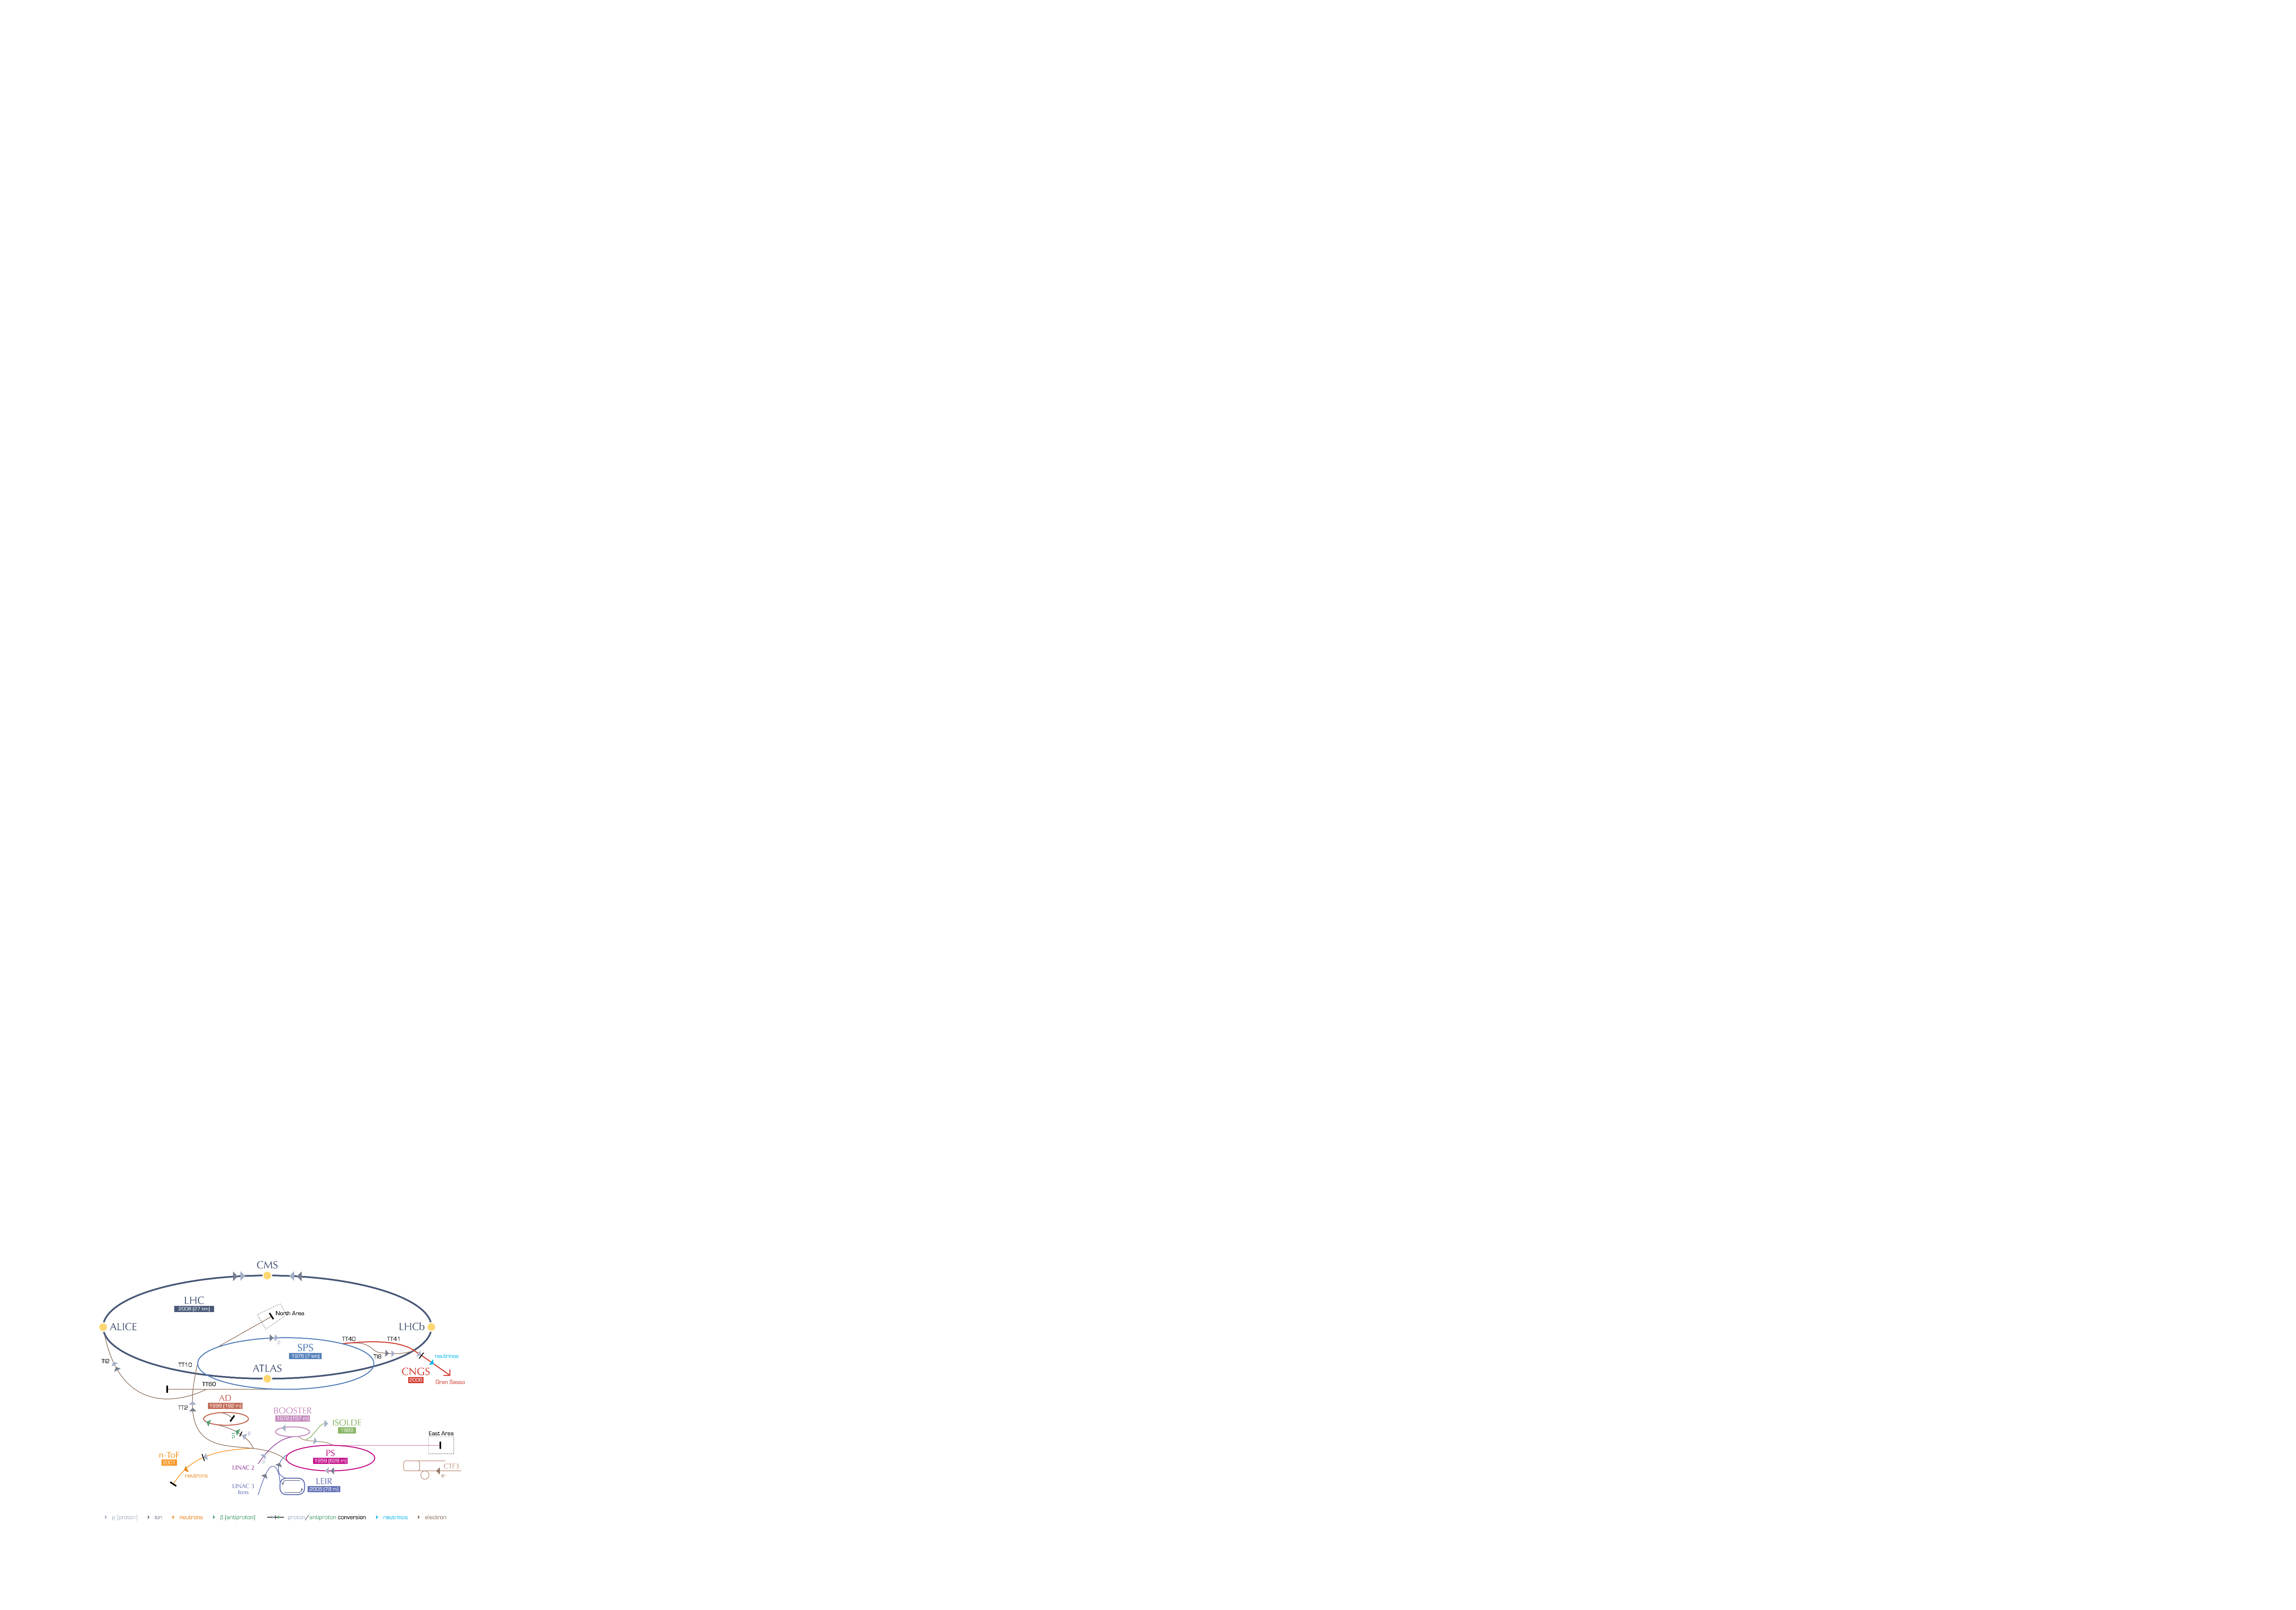
\includegraphics[width=1.0\textwidth]{figs/Detector/Acc_complex.pdf}
    \caption{The accelerator complex at \cern.}
    \label{fig:Dec_Acc_Complex}   
\end{figure}
%%%%%%%%%%%%%%%%%%%%%%%%%%%%%%%%%%%%%%%%%%%%%%%%%%%%%%%%%%

In addition to protons, the complex can accelerate other ions including lead, and more recently, xenon. These start in a dedicated linear accelerator, LINAC3, where the electrons are stripped off the ions to produce bare nuclei before being injected into the Low Energy Ion Ring (LEIR). This ring raises the ion's energy from 4.2\mev to 72\mev. 

Either protons or ions can then be injected in the Proton Synchrotron (PS), \cern's first synchrotron. Once the world's highest energy particle accelerator, this now accelerates the particles up to 25\gev ready to be injected into the Super Proton Synchrotron (SPS).
The SPS is the second largest accelerator at \cern, with a circumference of 7\km. It was switched on in 1976 and resulted in the notable discoveries of the \W and \Z bosons. Here, the particles are finally accelerated up to an energy of 450\gev, ready for injection into the \lhc. The particles are transferred from the SPS to the \lhc via two lines, one for each of the \lhc beam directions. The two beams, referred to as Beam 1 and Beam 2, travel clockwise and anti-clockwise respectively when viewed from above. Beam 2 is injected just before the \lhcb detector. 

The particles travel through the accelerator complex in groups called bunches. These typically contain around $10^{11}$ protons and are necessary as a result of the Radio-frequency (RF) cavities that accelerate the particles. The bunches are sequentially transferred between the accelerators in collections called trains. The bunch-trains are transferred from the SPS to the \lhc in a series of injections. Although the \lhc has a capacity for 3465 bunches, the nominal operating conditions has only 2808 of these spaces filled. 
These extra gaps allow enough room to safely divert the direction of the beam, without unintentionally damaging the instrumentation around the beam-pipe. The turn-on time for the magnets responsible for dumping the beam in emergencies is longer than the nominal 25\ns bunch spacing. 


Once the \lhc is at capacity the beams are accelerated from the injection energy of 450\gev to the nominal energy of up to 7\tev. This is achieved using eight RF cavities per beam to increase the beam energies and 1232 superconducting dipole magnets that bend the trajectory of the charged particles, ensuring they follow the paths dictated by the circular tunnels. The 15\m long dipole magnets contain superconducting niobium-titanium cables, kept cool at 1.9\,K using super-fluid helium. The 11,850\,A current flowing through the magnets generates a large magnetic field of 8.33\,T. The current is gradually and synchronously ramped as the particles are accelerated, such that the same curvature trajectory is maintained. 

The \lhc contains a wealth of other magnets, another 8,361 in addition to the dipole magnets, that optimise the orbit of the beams. This includes ensuring the beams remain tightly packed together, as well as many higher order corrections.   

During the injection and acceleration phase no collisions take place. Once the beams are at the nominal energy and beam profiles have been optimised, the two are brought together at four interaction points around the ring. Magnets are used to both redirect the beams such that they crossover and to squeeze the beams to a smaller cross-section at the collision points, increasing the likelihood of collisions. Once the beams overlap and the particles collide the experiments located around the four interaction points can begin to record data. The collisions typically continue for a duration of 10--20\hr (referred to as a fill). The number of particles in the bunches reduce, or \emph{burn-off}, as they collide with one another and the beam-pipes. A fill ends when the beams are intentionally or unintentionally dumped. The beam dumps are large graphite blocks surrounded by concrete shielding, designed to absorb the energy of the beams.  

A total of seven experiments are located at the \lhc, situated in four caverns. The four largest are \atlas, \cms, \lhcb and \alice. The TOTEM, LHCf and MoDEL experiments are located in the same caverns as \cms, \atlas and \lhcb respectively. 


%\subsection{The \lhcb collaboration} 



\subsection{Beam conditions}
The beam conditions at the \lhc have varied between the different years of data taking included in this thesis. A summary of some key parameters are detailed in Table~\ref{tab:Dec_phys_params}. This also includes the nominal conditions for the \lhc, for which it was designed. 


\begin{table}[h]
    \centering
      \begin{tabular}{lccccc}
         \hline
         Condition                                      & 2011      & 2012      & 2015      & 2016      & Nominal   \\ 
         \hline
         $\sqrt{s}$ (\tev)                              & 7         & 8         & 13        & 13        & 14        \\ 
         Peak luminosity ($10^{33}\cm^{-2} \sec^{-1}$)  & 3.5       & 7.6       & 4.8       & 14        & 12        \\ 
         Bunches                                        & 1380      & 1380      & 1368      & 2736      & 2808      \\ 
         Bunch spacing (\ns)                            & 50        & 50        & 25        & 25        & 25        \\ 
         \hline
         Average $N_{\text{collisions}}$, $\mu$         & 1.7       & 1.7       & 1.1       & 1.1       & -         \\ 
         Integrated luminosity (\invfb)                 & 1.0       & 2.0       & 0.3       & 1.5       & -         \\ 
         \hline
      \end{tabular}
   \caption{Beam conditions in the different datasets used in this thesis. The last two rows are specific to \lhcb.}
   \label{tab:Dec_phys_params}
\end{table}


During a normal fill the luminosity delivered to the large experiments slowly decreases as the protons burn off. For \atlas and \cms the average number of collisions per bunch crossing (known as pile up) is high: around 27 in 2016. 
The \lhcb experiment chooses to level the luminosity to a lower value than the maximum achievable. This means the average number of visible collisions per bunch crossing, $\mu$, is much lower, between 1.1 and 1.7 depending on the year. The same luminosity is maintained for the majority of a fill via a process know as luminosity levelling. At the beginning of the fill the two beams are vertically separated from one another such that the overlap between them is not maximised. As the fill progresses the two beams are brought closer together to compensate for the burn off of the bunches. This way a constant instantaneous luminosity of between (2--4)$\times 10^{32} \cm^{2} \sec^{-1}$ can be maintained thorough out the given fill.

In addition to the luminosity levelling, the two beams collide at an angle in the horizontal plane. This helps to reduce unwanted collisions between the bunches either side of the intended collision bunches. The angle of collision depends on the polarity of the \lhcb spectrometer magnet as the dipole field affects beam-steering fields around the interaction point. 


% {\color{Red}
% \begin{itemize}
% \item \lhc optics
% \item crossing angle
% \end{itemize}
% }


\section{The \lhcb detector}

This section provides an overview of the experimental apparatus used to obtain the data analysed in this thesis.
The \lhcb detector is comprised of distinct sub-detectors, each with a dedicated purpose. These help to characterise the sub-atomic particles created in the proton-proton collisions, and enable measurements of their kinematics, trajectories and species.
This overview includes a description of the sub-detector's principles, components and performance. 

The \lhcb detector is found at Point 8 of the \lhc ring, in a cavern originally built for the \delphi detector during the \lep era. A schematic representing the key components of the \lhcb detector is shown in Fig.~\ref{fig:Dec_lhcb_Schematic}. This figure displays the axes convention adopted by \lhcb, and used henceforth. The horizontal axis is labelled the $z$-axis and is parallel to the direction of the beams. The figure's vertical axis is the $y$-axis, increasing as one moves from the cavern up to ground level. The $x$-axis is in the dimension perpendicular to the plane of the figure and increases as one moves towards the centre of the \lhc ring. The counter-rotating beams of protons are collided at the far left of this figure, at the origins of the $y$- and $z$-axes.   

%%%%%%%%%%%%%%%%%%%%%%%%%%%%%%%%%%%%%%%%%%%%%%%%%%%%%%%%%%
\begin{figure}[!h]
    \centering
    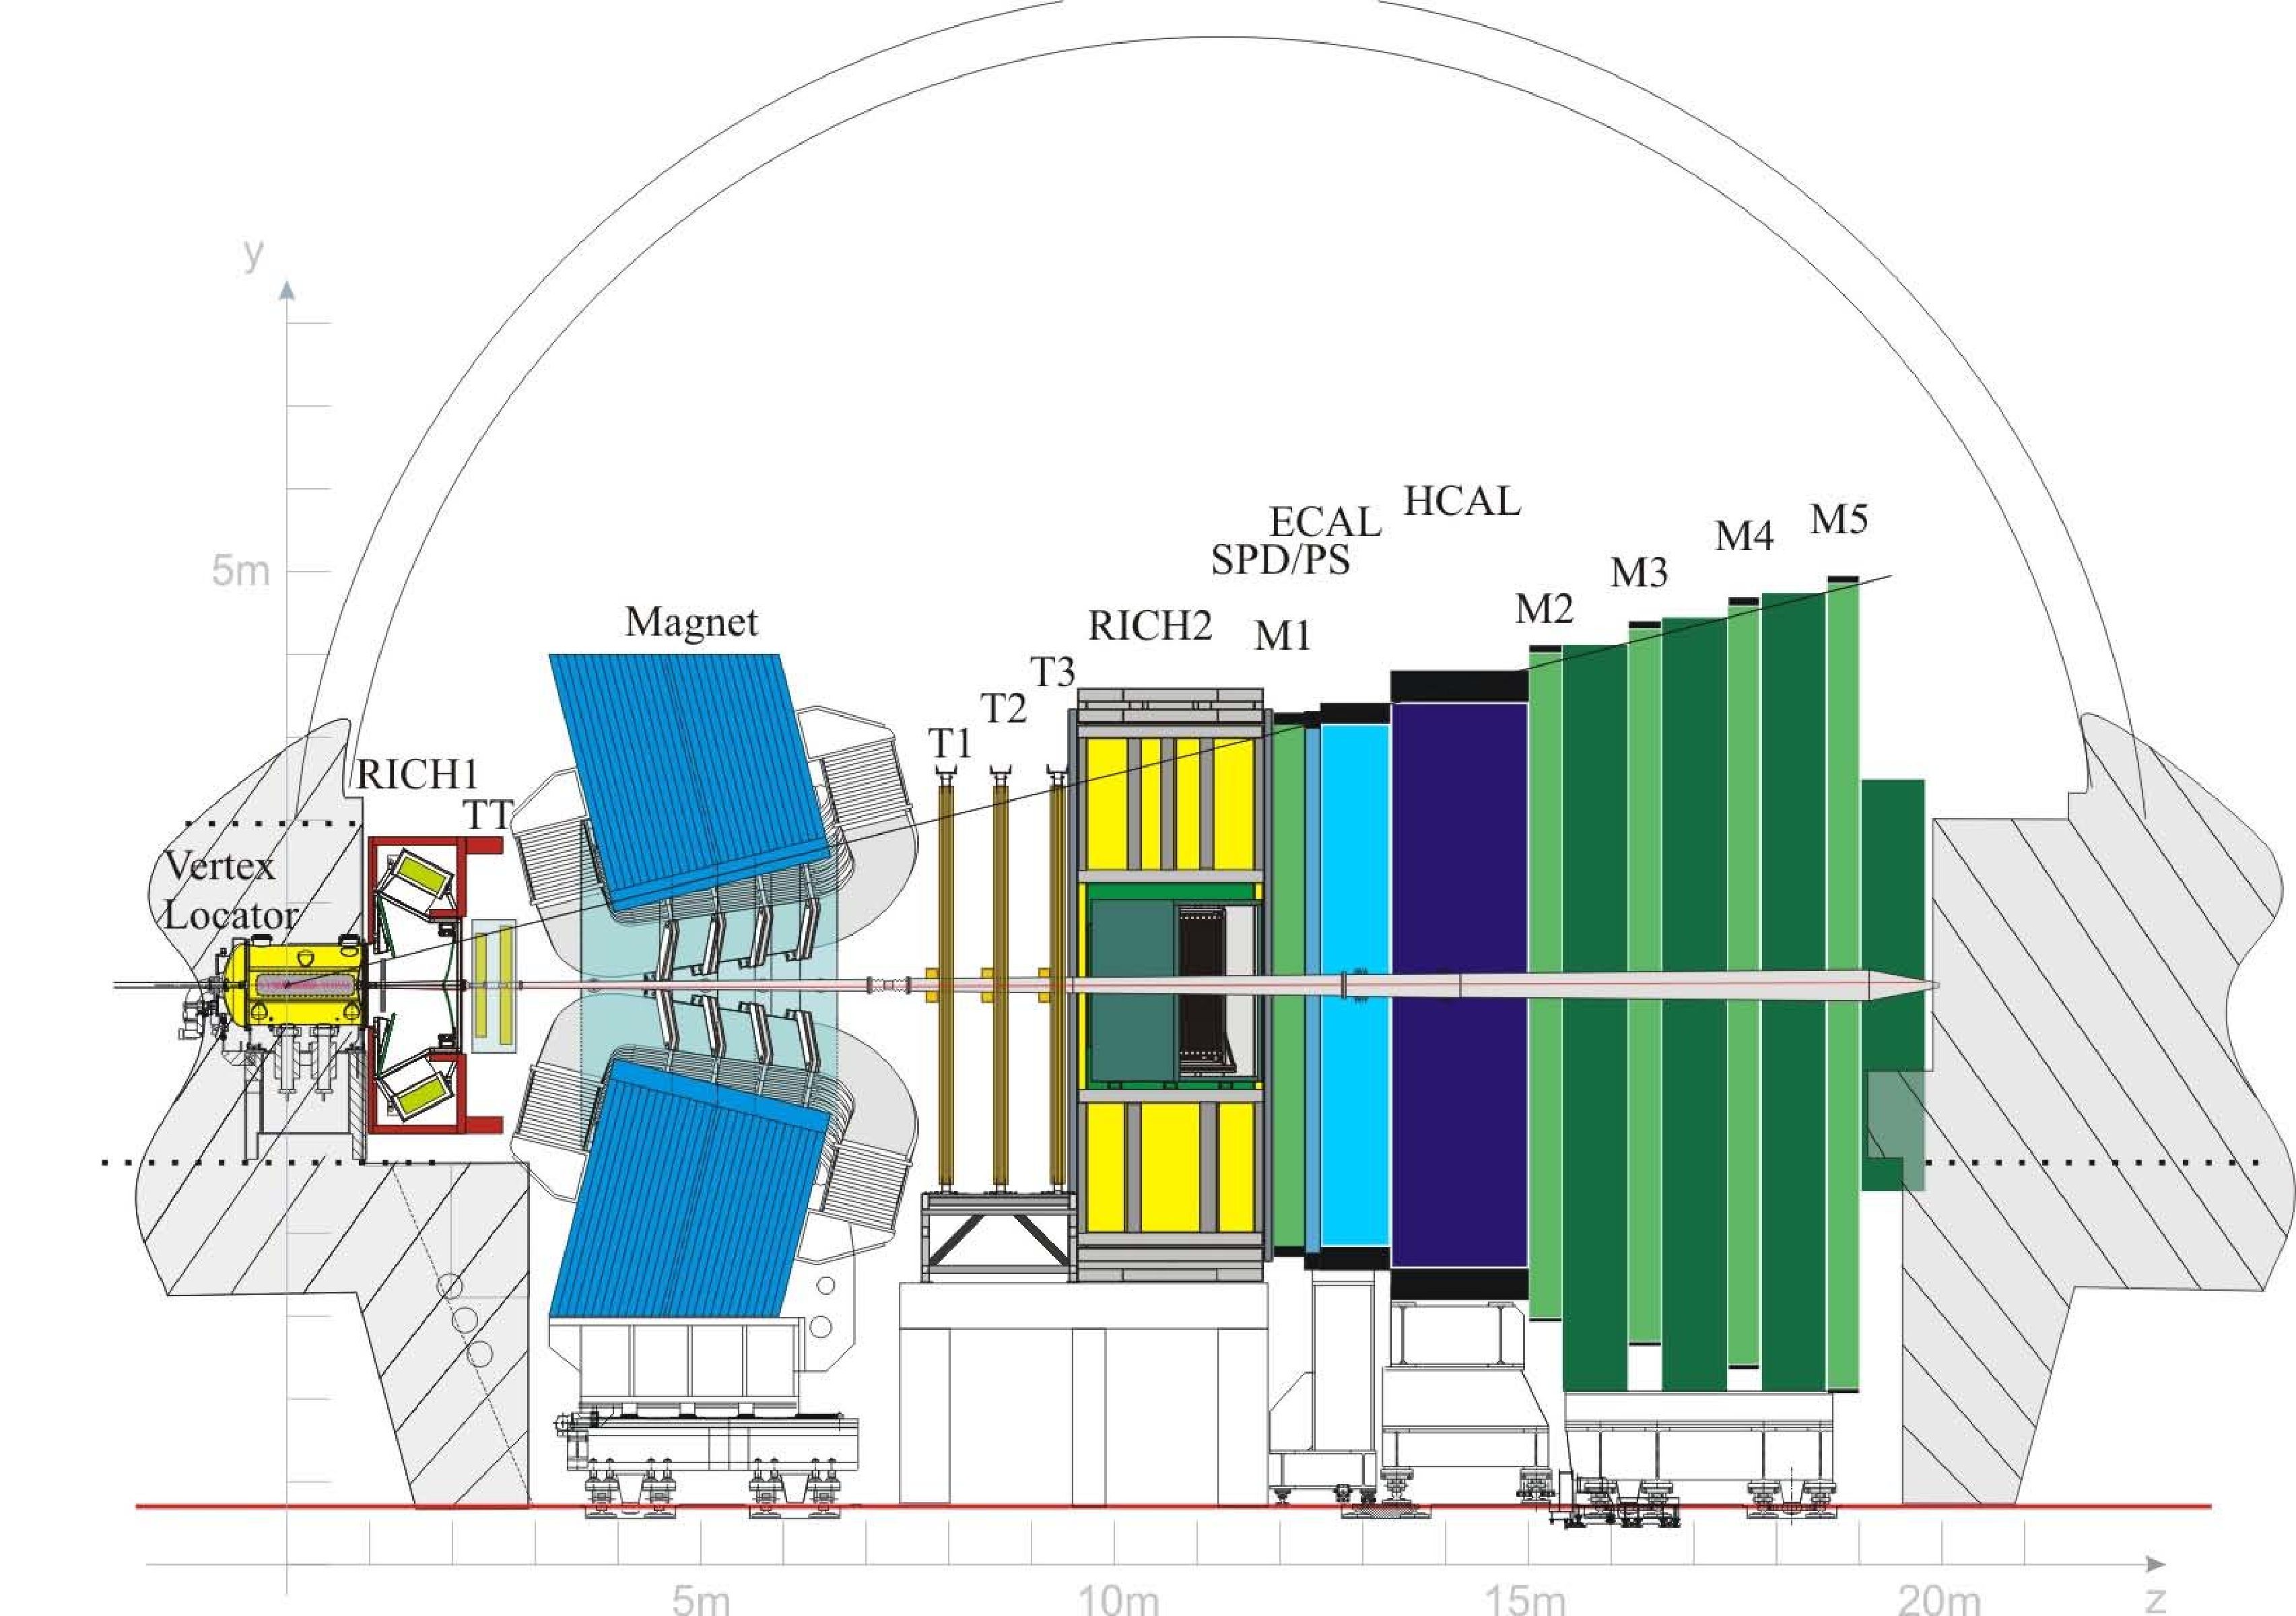
\includegraphics[width=0.8\textwidth]{figs/Detector/LHCb_Detector_Schematic.pdf}
    \caption{Schematic of the \lhcb detector, from Ref.~\cite{Alves:2008zz}.}
    \label{fig:Dec_lhcb_Schematic}   
\end{figure}
%%%%%%%%%%%%%%%%%%%%%%%%%%%%%%%%%%%%%%%%%%%%%%%%%%%%%%%%%%

The \lhcb detector covers only a small fraction of the area around the collision region; the acceptance covers particles with a pseudo-rapidity in the range $1.8 < \eta < 4.9$ on one side of the interaction point. However, this configuration is well suited to the reconstruction of particles containing \bquark or \bquarkbar quarks. The angular distribution of \bquark\bquarkbar pairs is shown in Fig.~\ref{fig:Dec_bb_production}, along with the acceptance of \lhcb in red. The distribution is highly peaked towards the forward and backward regions as \bquark-hadrons tend to receive large boosts at this collision energy. Approximately 25\% of decays have both \bquark and \bquarkbar quarks produced inside the acceptance.

% %%%%%%%%%%%%%%%%%%%%%%%%%%%%%%%%%%%%%%%%%%%%%%%%%%%%%%%%%%
\begin{figure}[!h]
    \centering
    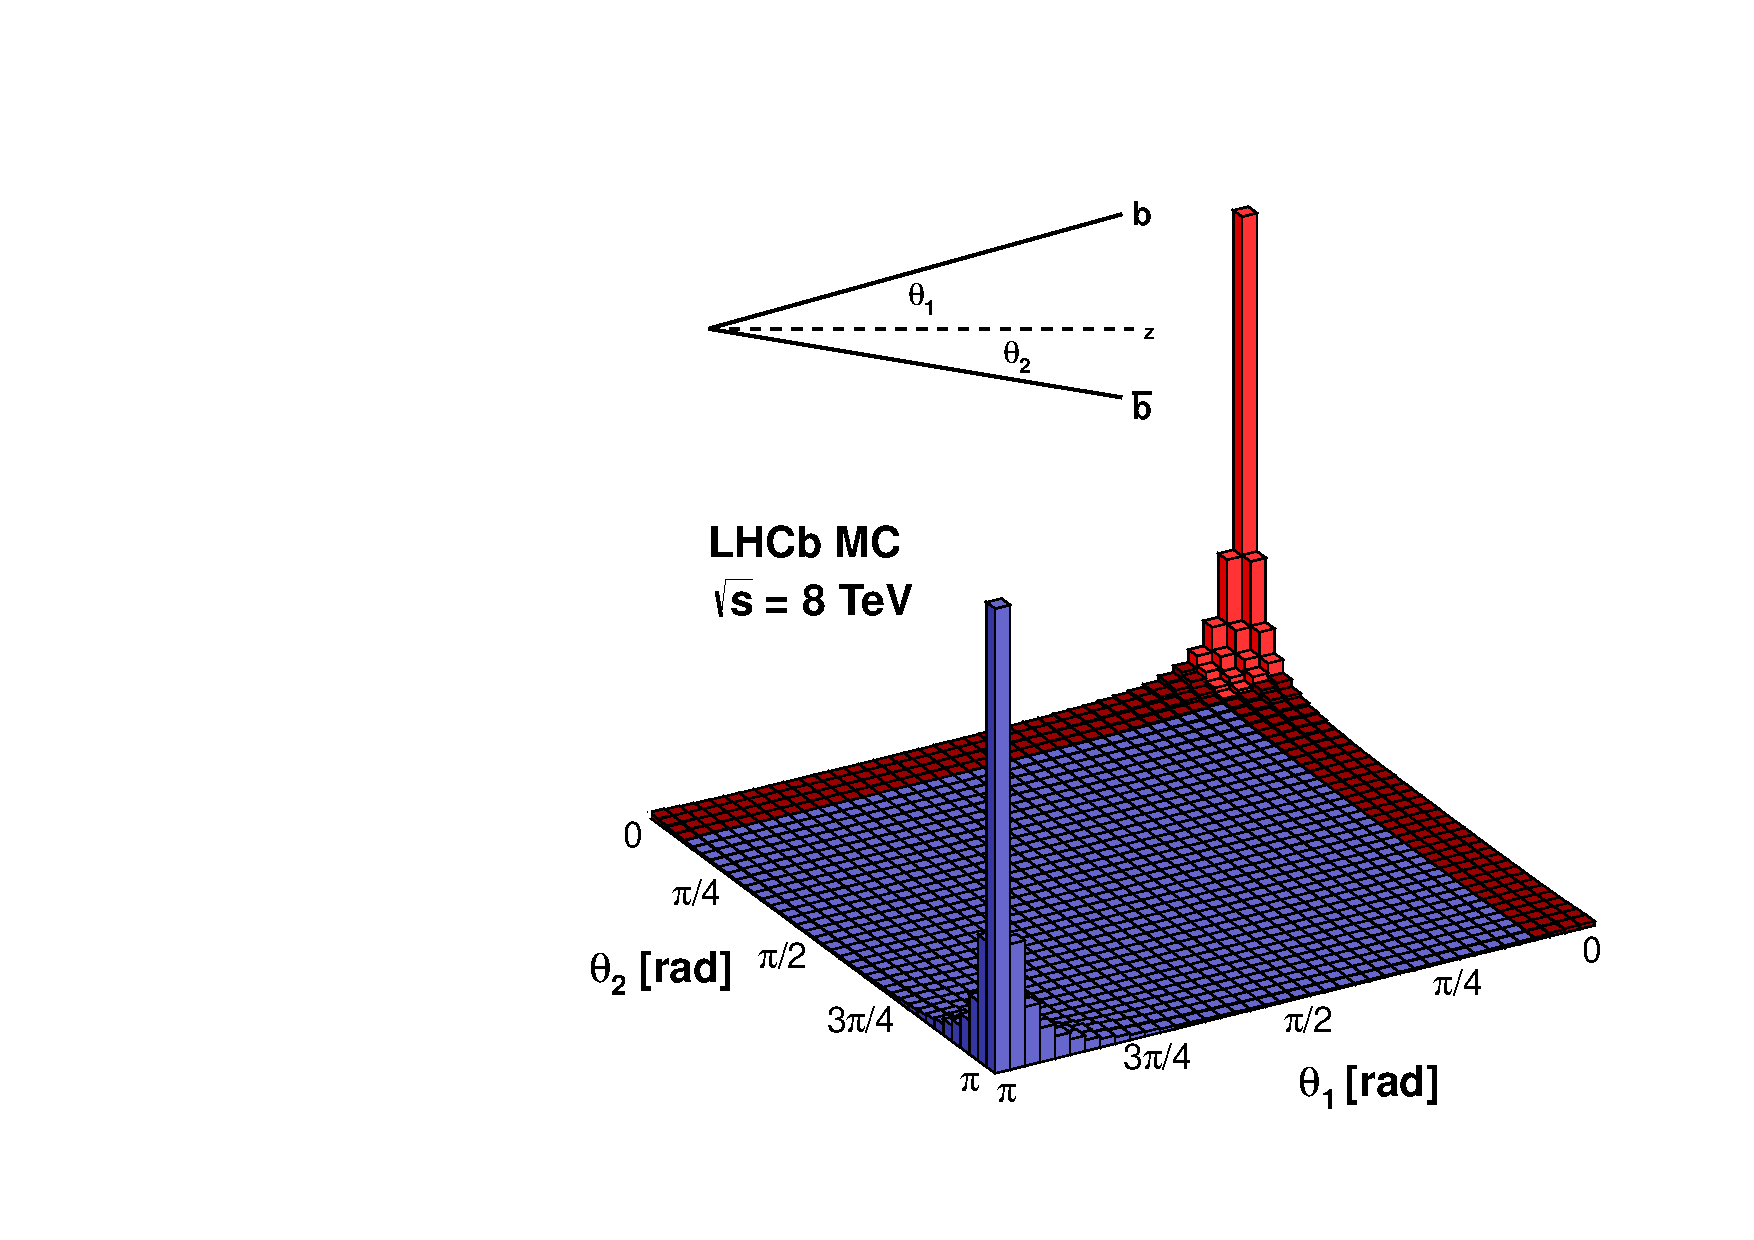
\includegraphics[width=0.6\textwidth]{figs/Detector/bb_acceptance.pdf}
    \caption{The angular distribution of \bquark\bquarkbar pair production in simulated \proton \proton collisions at a centre-of-mass energy of 8\,TeV. The acceptance of \lhcb is highlighted in red.}
    \label{fig:Dec_bb_production}   
\end{figure}
% %%%%%%%%%%%%%%%%%%%%%%%%%%%%%%%%%%%%%%%%%%%%%%%%%%%%%%%%%%


Running along the centre of the detector is the \lhcb beampipe. The primary role is to separate the inner vacuum chamber from the rest of the cavern, allowing the beams to proceed unimpeded by the air. The majority of the beampipe is made of beryllium, with smaller sections made out of aluminium alloys or stainless steel. Although beryllium is a highly toxic and fragile material it has a long radiation length, allowing the incident particles to traverse the pipe walls with minimal interactions.  


\subsection{Magnet}

The \lhcb detector contains a warm dipole magnet that bends the trajectories of charges particles, allowing measurements of the particles' momentum. The magnet has two saddle-shaped coils inside a square yoke that generate an integrated magnetic field of 4\,Tm.  
The magnetic field is aligned along the $y$-axis, bending the charged particles in the horizontal plane. The polarity of the magnetic is routinely switched during data taking. This helps to understand and cancel systematic effects that may affect measurements of \CP asymmetries. The two magnet polarities are referred to \MagDown and \MagUp, corresponding to a field in the negative and positive $y$-axis direction respectively.   

A schematic of the magnet is shown in Fig.~\ref{fig:Dec_magnet}, along with the strength of the magnetic field as a function of the $z$-axis position. Both magnet polarities are represented in this figure. 


%%%%%%%%%%%%%%%%%%%%%%%%%%%%%%%%%%%%%%%%%%%%%%%%%%%%%%%%%%
\begin{figure}[!h]
    \centering
    \begin{subfigure}[t]{0.4\textwidth}
        \centering
        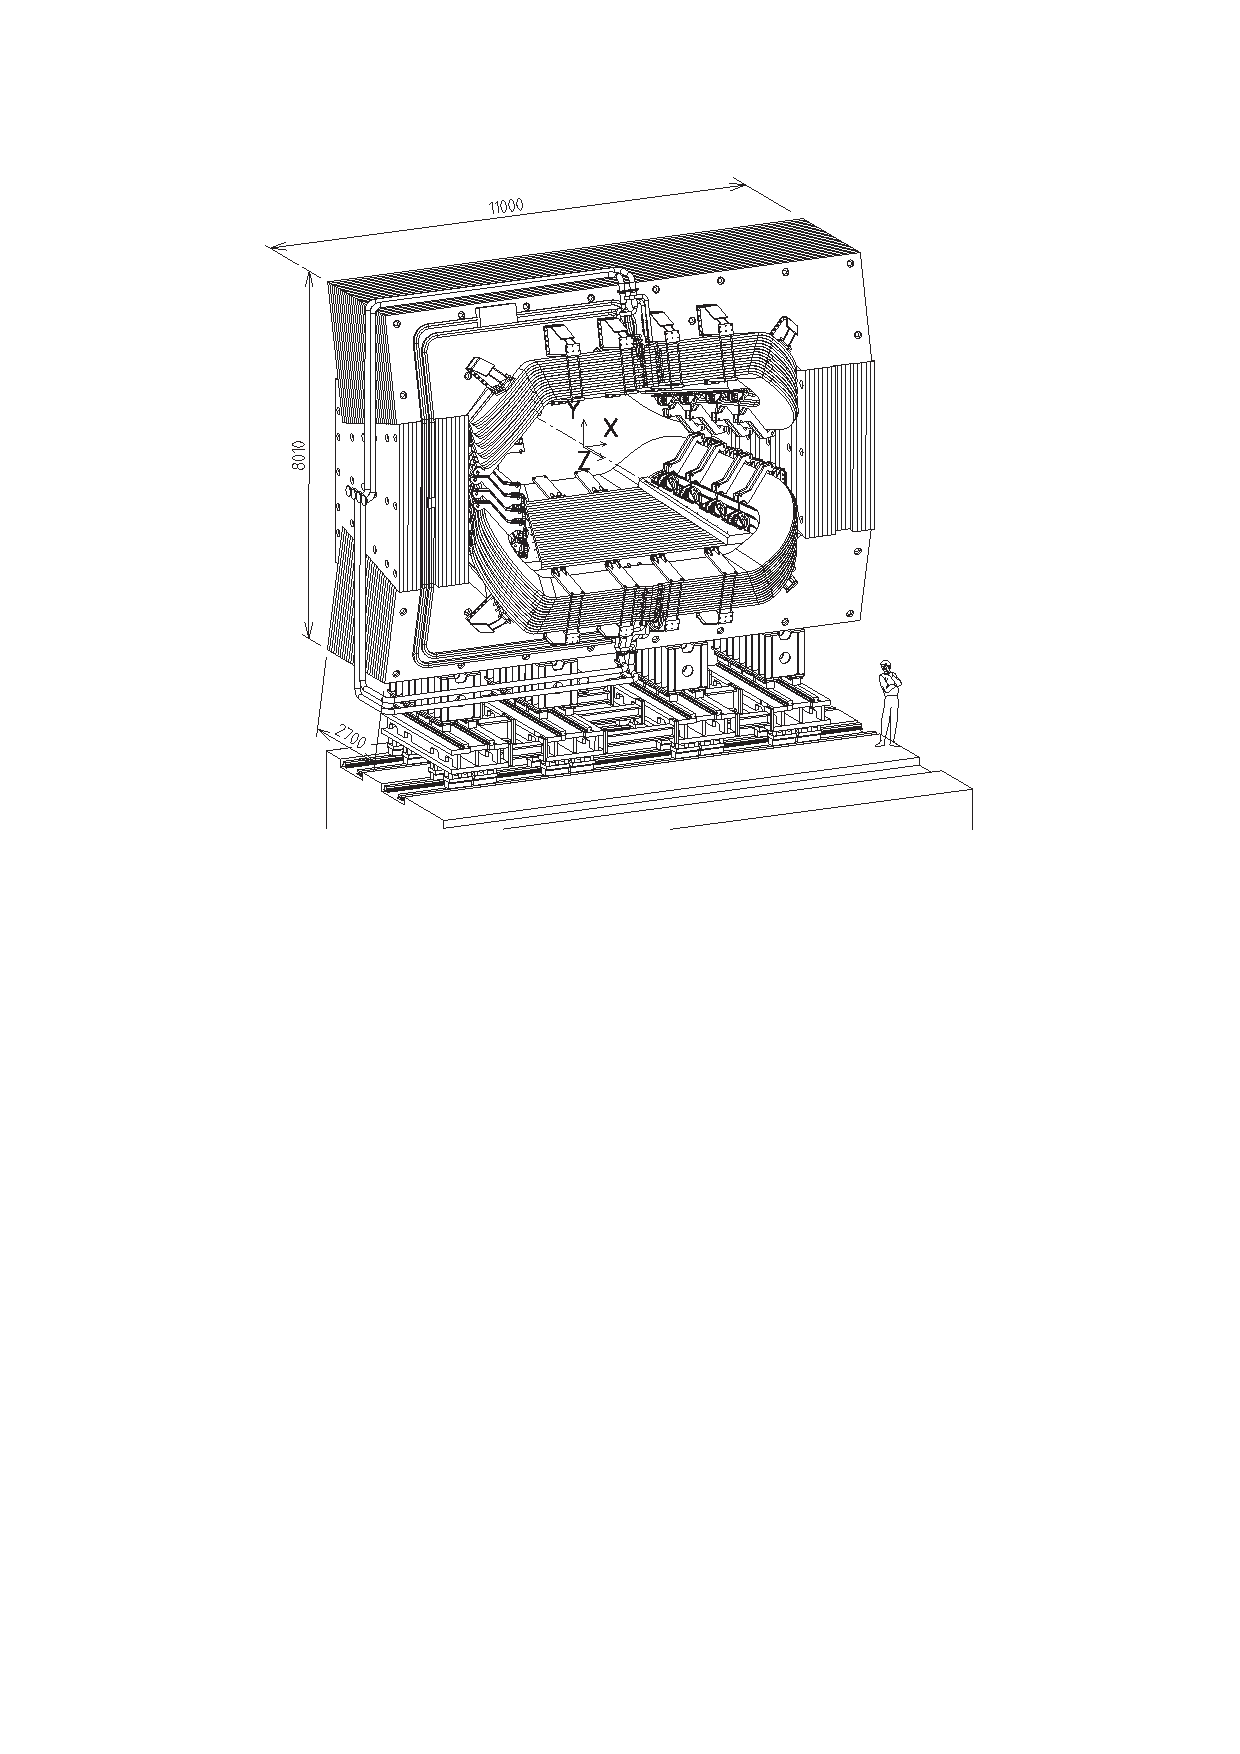
\includegraphics[width=1.0\textwidth]{figs/Detector/magnet_schematic.pdf}
    \end{subfigure}
    \begin{subfigure}[t]{0.4\textwidth}
        \centering
        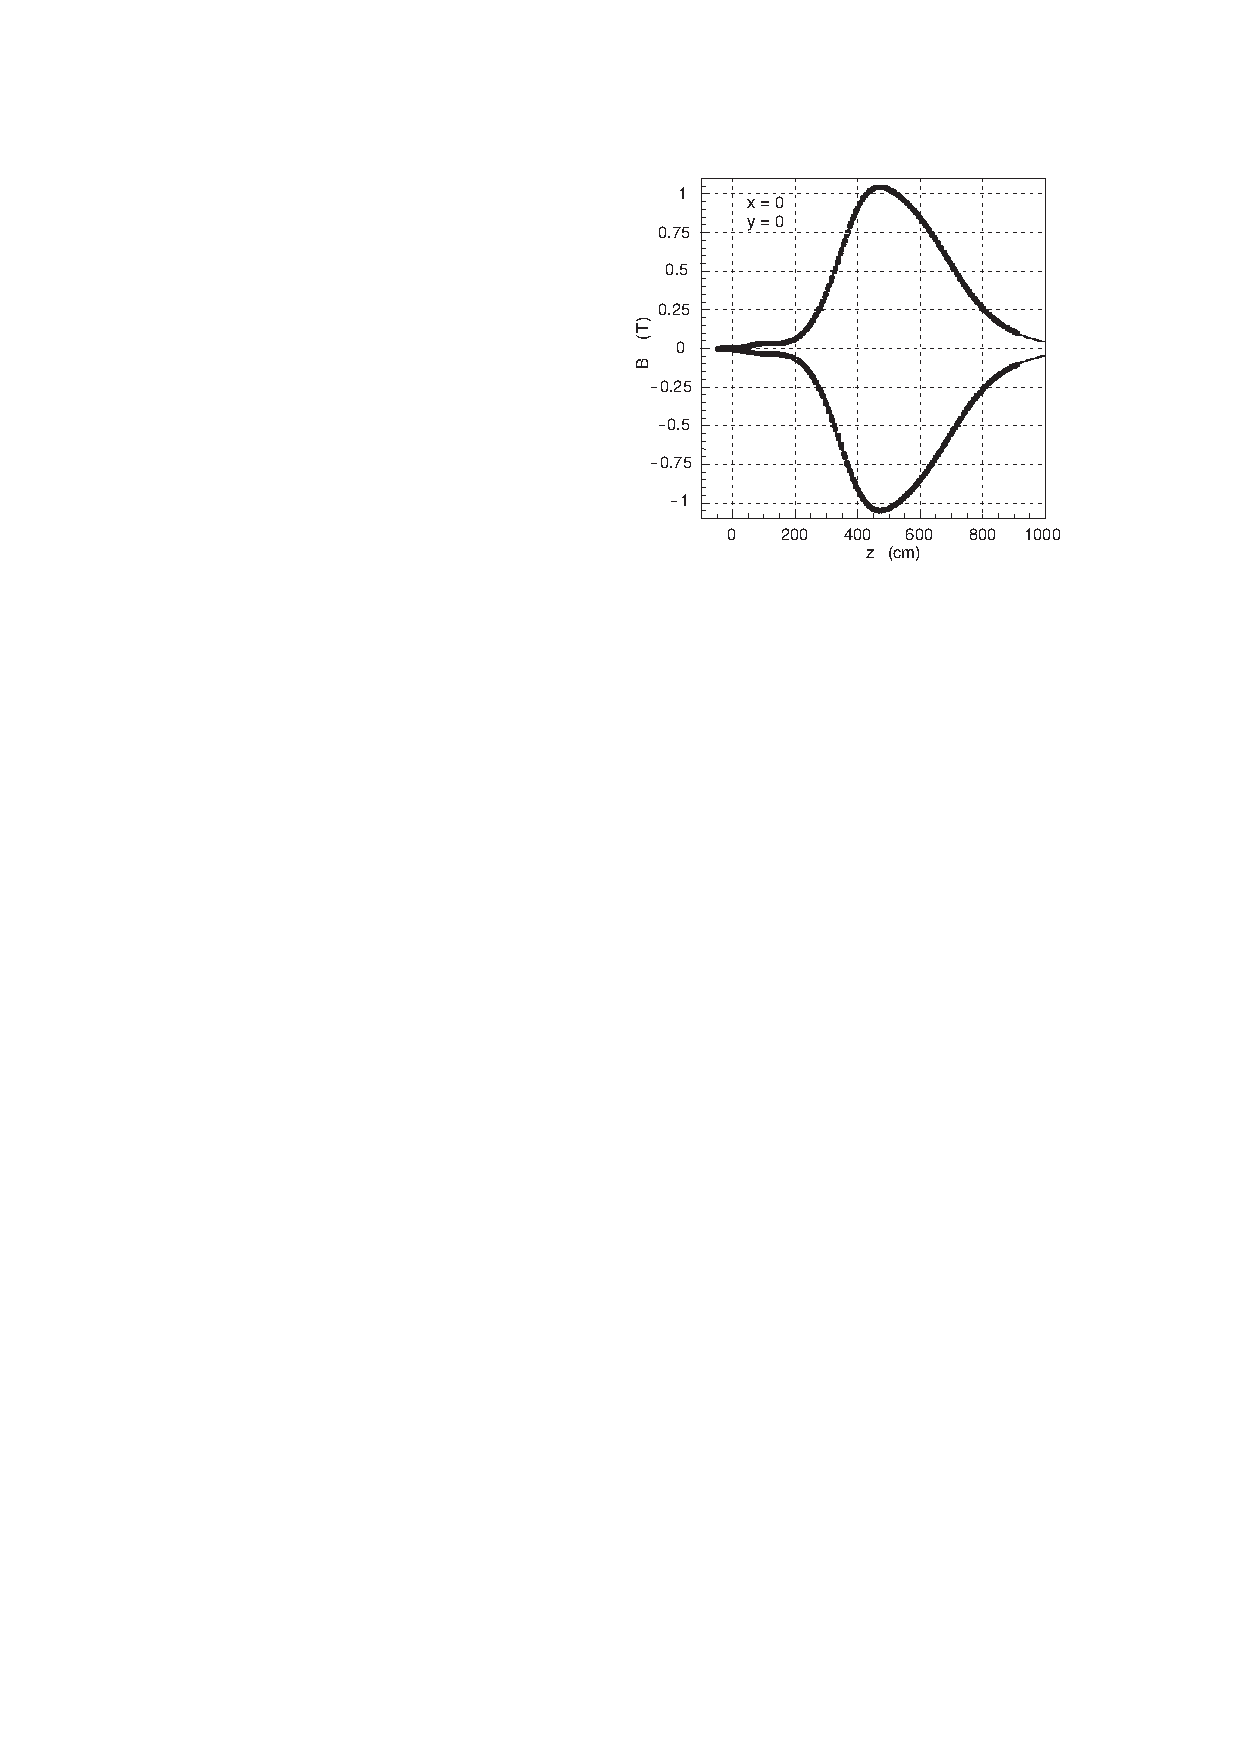
\includegraphics[width=1.0\textwidth]{figs/Detector/magnet_B_field.pdf}
    \end{subfigure}
    \caption{Schematic of the \lhcb warm dipole magnet (left) and the magnetic field strength along the $z$-axis (right) from Ref.~\cite{Alves:2008zz}.}
    \label{fig:Dec_magnet}   
\end{figure}
%%%%%%%%%%%%%%%%%%%%%%%%%%%%%%%%%%%%%%%%%%%%%%%%%%%%%%%%%%


\subsection{Vertex Locator}

The first sub-detector to make measurements of the particles produced in proton-proton collisions is the Vertex Locator (\velo) encompassing the collision region. This sub-detector makes precise measurements of the track positions of charged particles as they emanate out of the collisions. A high level of precision is required to identify the secondary vertices characteristic of \bquark- and \cquark-hadron decays. These secondary vertices are typically displaced from the interaction position as a result of the long lifetimes associated to these heavy-flavour hadrons. This is achieved by measuring the track coordinates using silicon strip sensors placed as close to the \lhc beam as safety allows. The \velo sensors are semicircular devices placed on either side of the beam. To allow the sensors to instrument the innermost region around the interaction point the two halves of the \velo can move horizontally in and out. During normal data taking this allows the sensors to be 7\mm away from the interaction point yet still be a safe distance away from the beams at injection. 

%%%%%%%%%%%%%%%%%%%%%%%%%%%%%%%%%%%%%%%%%%%%%%%%%%%%%%%%%%
\begin{figure}[!h]
    \centering   
    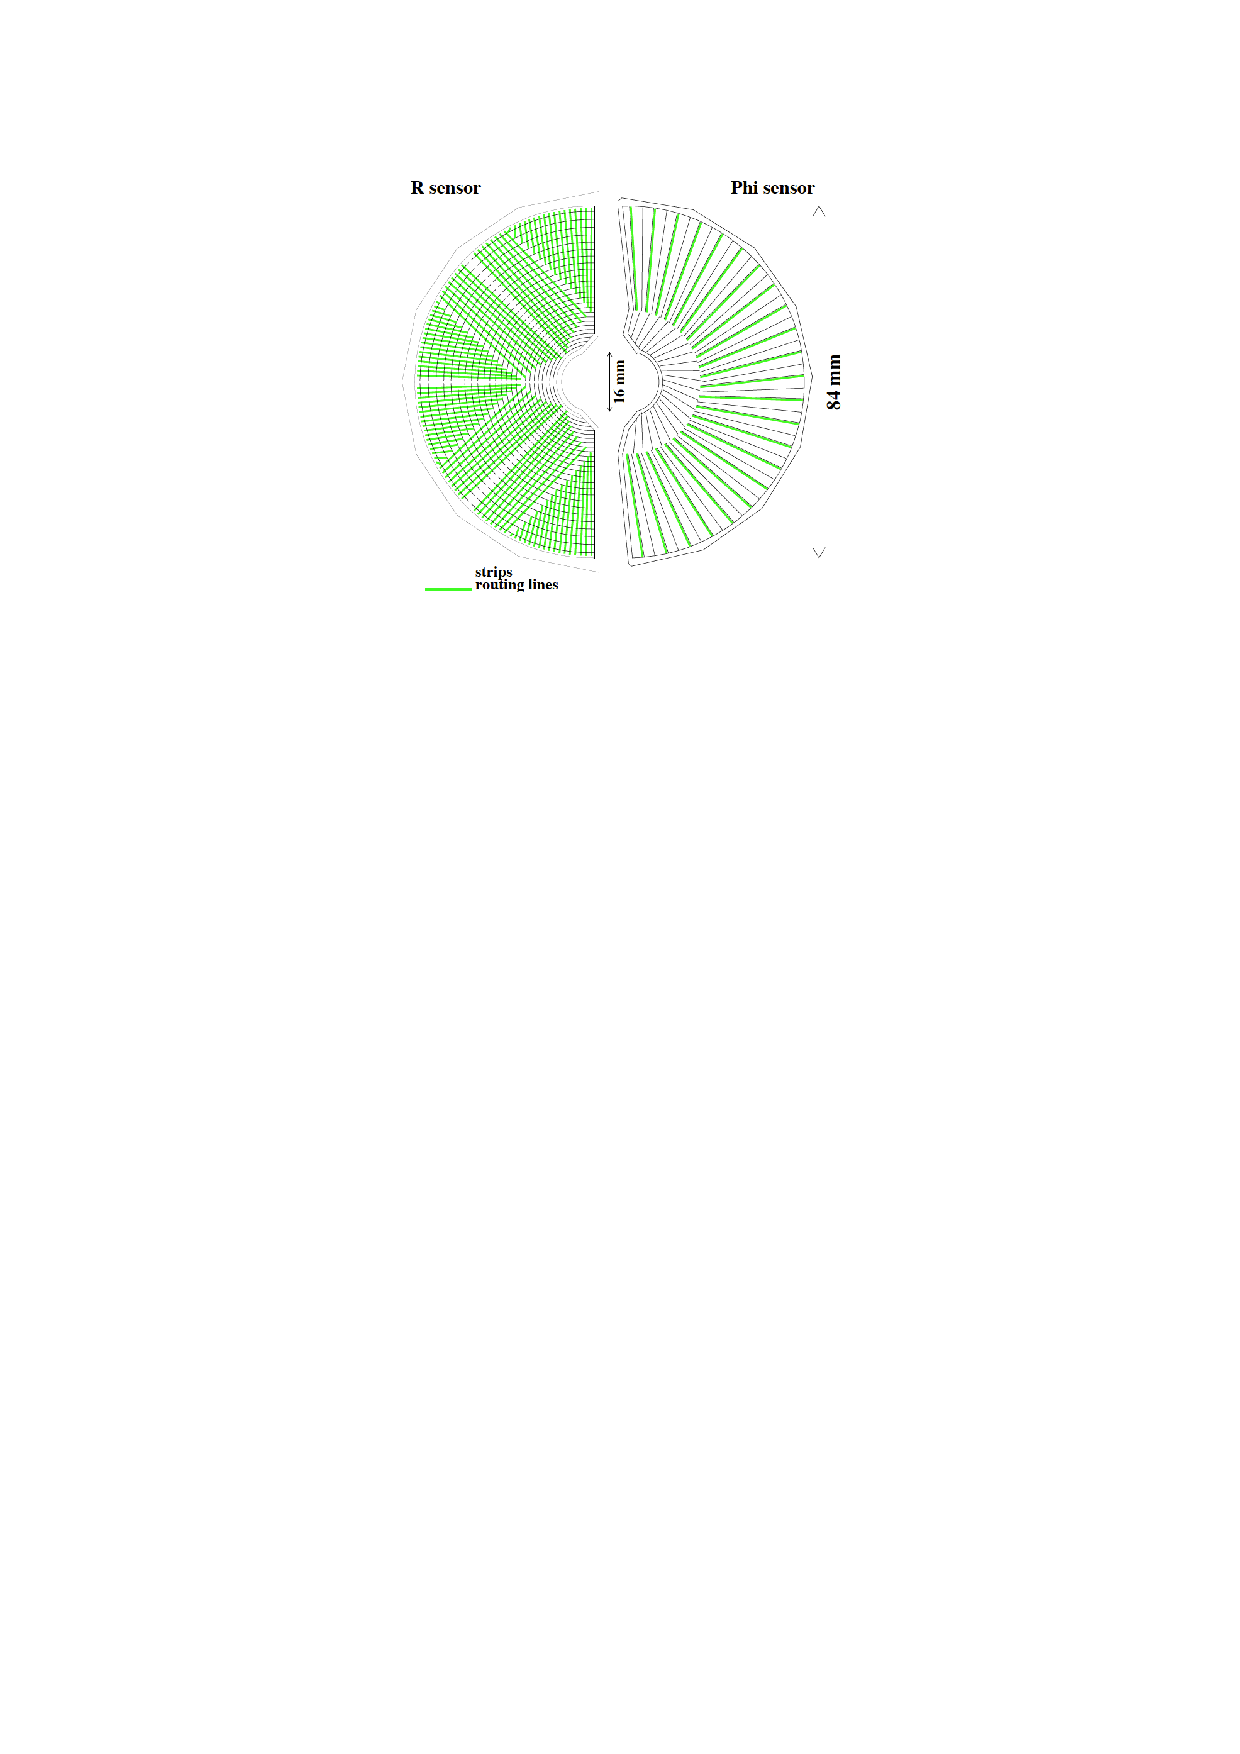
\includegraphics[width=0.4\textwidth]{figs/Detector/velo_r_phi_sensor.pdf}
    \caption{Schematic of an $r$- and $\phi$-sensor in the \velo sub-detector, from Ref.~\cite{LHCb-DP-2014-001}.}
    \label{fig:Dec_r_phi_sensor}   
\end{figure}
%%%%%%%%%%%%%%%%%%%%%%%%%%%%%%%%%%%%%%%%%%%%%%%%%%%%%%%%%%

The sensors are grouped into pairs, called modules. Each of the 21 modules on each side contains sensors for measuring the radial and azimuthal coordinates of the tracks, referred to as $r$- and $\phi$-sensors respectively. A schematic of the two sensor types is shown in Fig.~\ref{fig:Dec_r_phi_sensor}, illustrating the silicon strips and readout channels. 


The \velo modules are arranged to ensure coverage of particles emerging in forward region at angles of 15--300\mrad with respect to the beam-pipe. This arrangement allows tracks within this acceptance to interact in at least three sensors as shown in Fig.~\ref{fig:Dec_velo_sensor_layout}.   
The modules extend both forward and backwards of the interaction region. Although momentum measurements are not possible for backward tracks, the vertexing of the primary interaction can benefit from this extra information. In the far backward region there are two additional modules, measuring only the radial coordinate. These help to identify pile-up events in which there is more than one primary vertex. 

%%%%%%%%%%%%%%%%%%%%%%%%%%%%%%%%%%%%%%%%%%%%%%%%%%%%%%%%%%
\begin{figure}[!h]
    \centering
    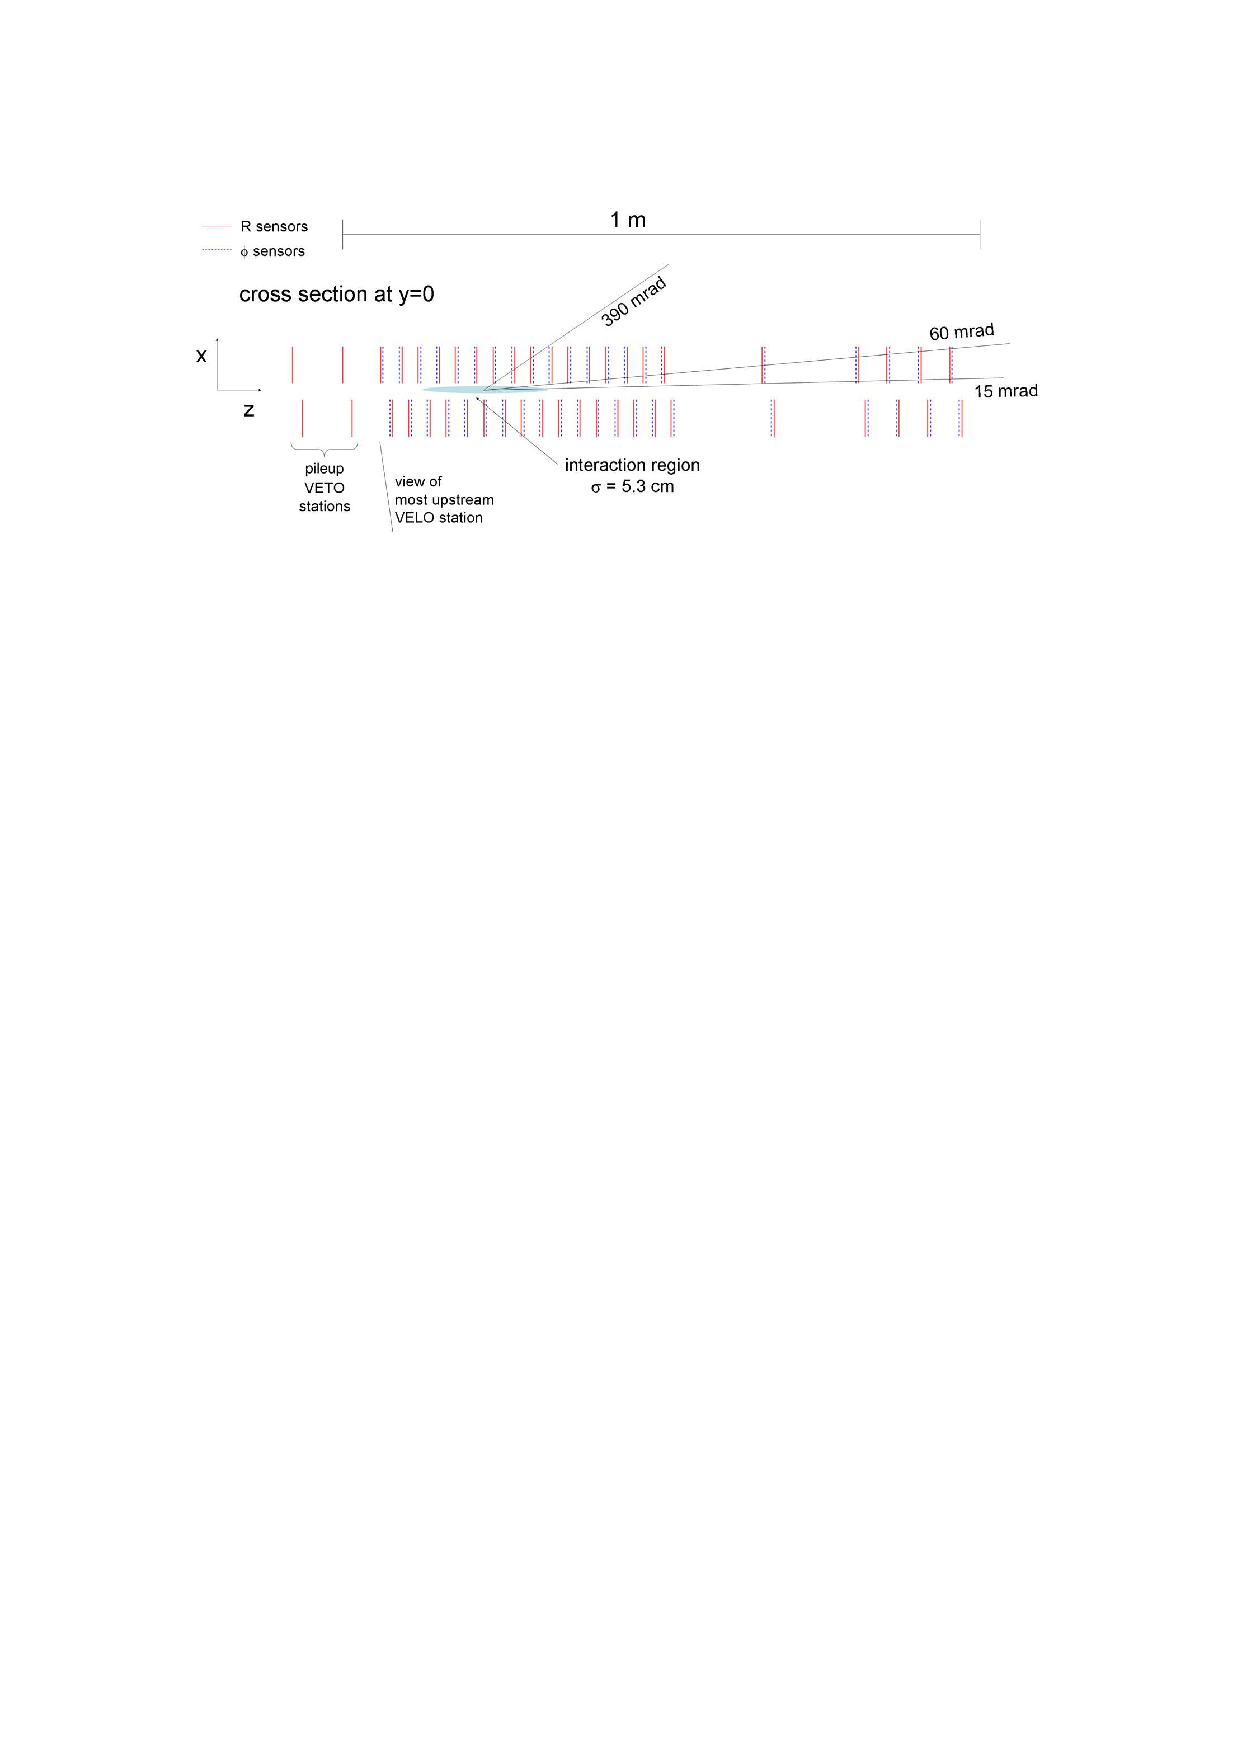
\includegraphics[width=0.8\textwidth]{figs/Detector/velo_sensor_layout.pdf}
    \caption{Schematic of the sensor layout in the \velo sub-detector, from Ref.~\cite{LHCb-DP-2014-001}.}
    \label{fig:Dec_velo_sensor_layout}   
\end{figure}
%%%%%%%%%%%%%%%%%%%%%%%%%%%%%%%%%%%%%%%%%%%%%%%%%%%%%%%%%%

The \velo sub-detector is constructed to operate in the unique environment close to the \lhc beams.
\begin{description}   
\item \textbf{Radiation resistance:} the \velo modules are subjected to extreme and varying amounts of radiation. The detector is designed to with stand three years of nominal \lhc running, using a radiation tolerant semiconductor construction. Additionally, the \velo modules are cooled to remove the heat created from the interactions. The sensors are maintained at a temperature between -10 and 0\degrees{C} with 24\,W of heat removed from each sensor.  
\item \textbf{Radio-frequency (RF) pick-up protection:} the electromagnetic fields generated by the \lhc beams could cause interference in the \velo detectors electronics. Therefore, a shield is used between the modules and the beam-pipe referred to as the RF-foil. This 0.3\mm thick foil separates the \velo and beam-pipe vacuums, providing additional protection to the conditions of the beams from the detector.
\end{description}   

The hits arising from particle interactions in the \velo sensors are extracted from the readout channels using custom analogue chips. The signals are digitised and combined into clusters in readout boards called \tellone boards~\cite{HAEFELI2006494}, 


The performance of the \velo sub-detector can be quantified using different metrics. Two of particular interest are the track finding efficiency and the resolution of the impact parameter of a track. 
The track finding efficiency determines the likelihood that a track will be reconstructed and is of particular importance for high multiplicity final states including those presented in this thesis. The average track finding efficiency in data taken during 2011 is found to be around 98\% as shown in Fig.~\ref{fig:Dec_velo_track_performance}.

The impact parameter (IP) represents the distance between a track and a primary vertex at the point of closest approach. Long-lived particles, such as \Bp mesons, decay at a secondary vertex displaced from the primary collision vertex. Therefore, the decay products of these particles have a larger IP that the tracks originating at the primary vertex. A precise measurement of the IP of a track allows the \Bp mesons and various background processes to be differentiated. The distribution of the $x$-component of the IP is shown as a function of the inverse transverse momentum ($1/\pt$) in Fig.~\ref{fig:Dec_velo_track_performance}.  

%%%%%%%%%%%%%%%%%%%%%%%%%%%%%%%%%%%%%%%%%%%%%%%%%%%%%%%%%%
\begin{figure}[!h]
    \centering
    \begin{subfigure}[t]{0.4\textwidth}
        \centering
        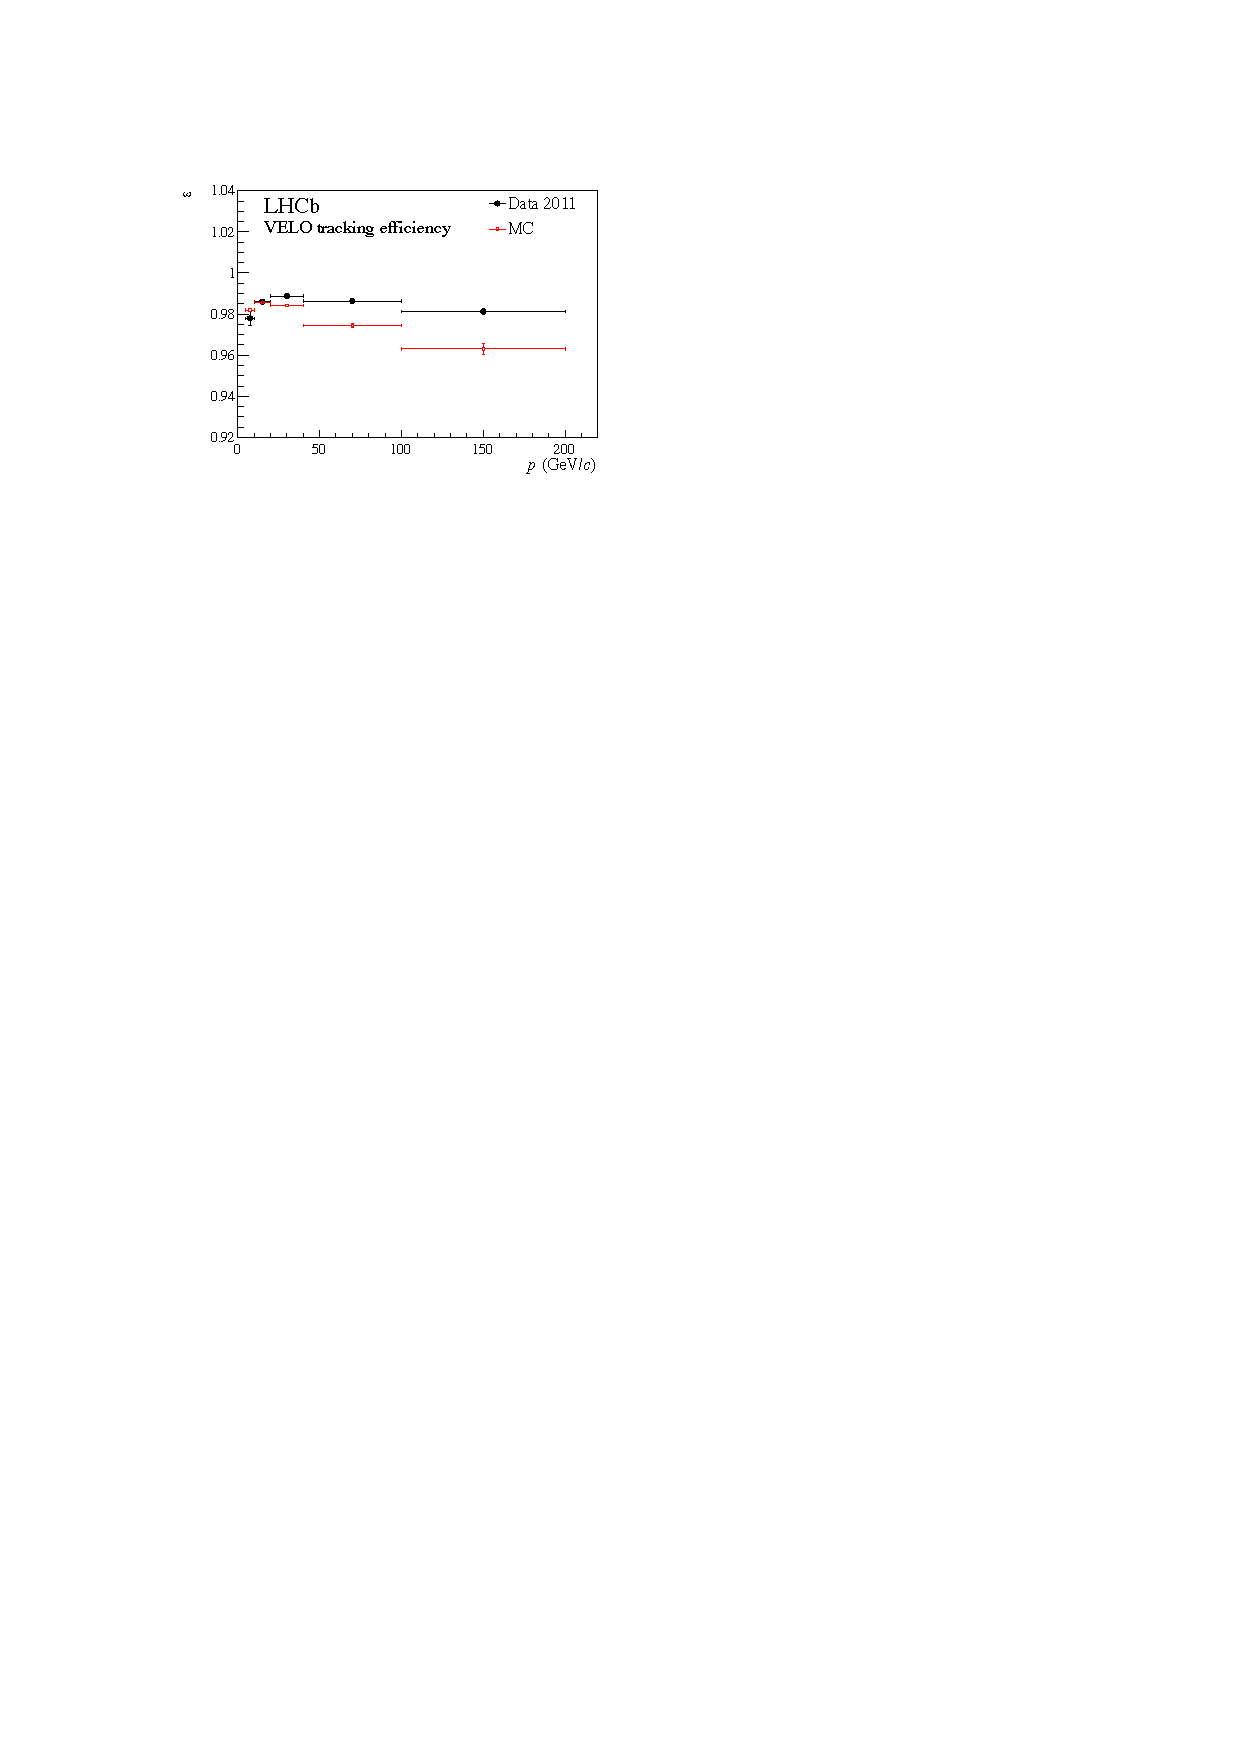
\includegraphics[width=1.0\textwidth]{figs/Detector/velo_track_eff_2011.pdf}
    \end{subfigure}
    \begin{subfigure}[t]{0.4\textwidth}
        \centering
        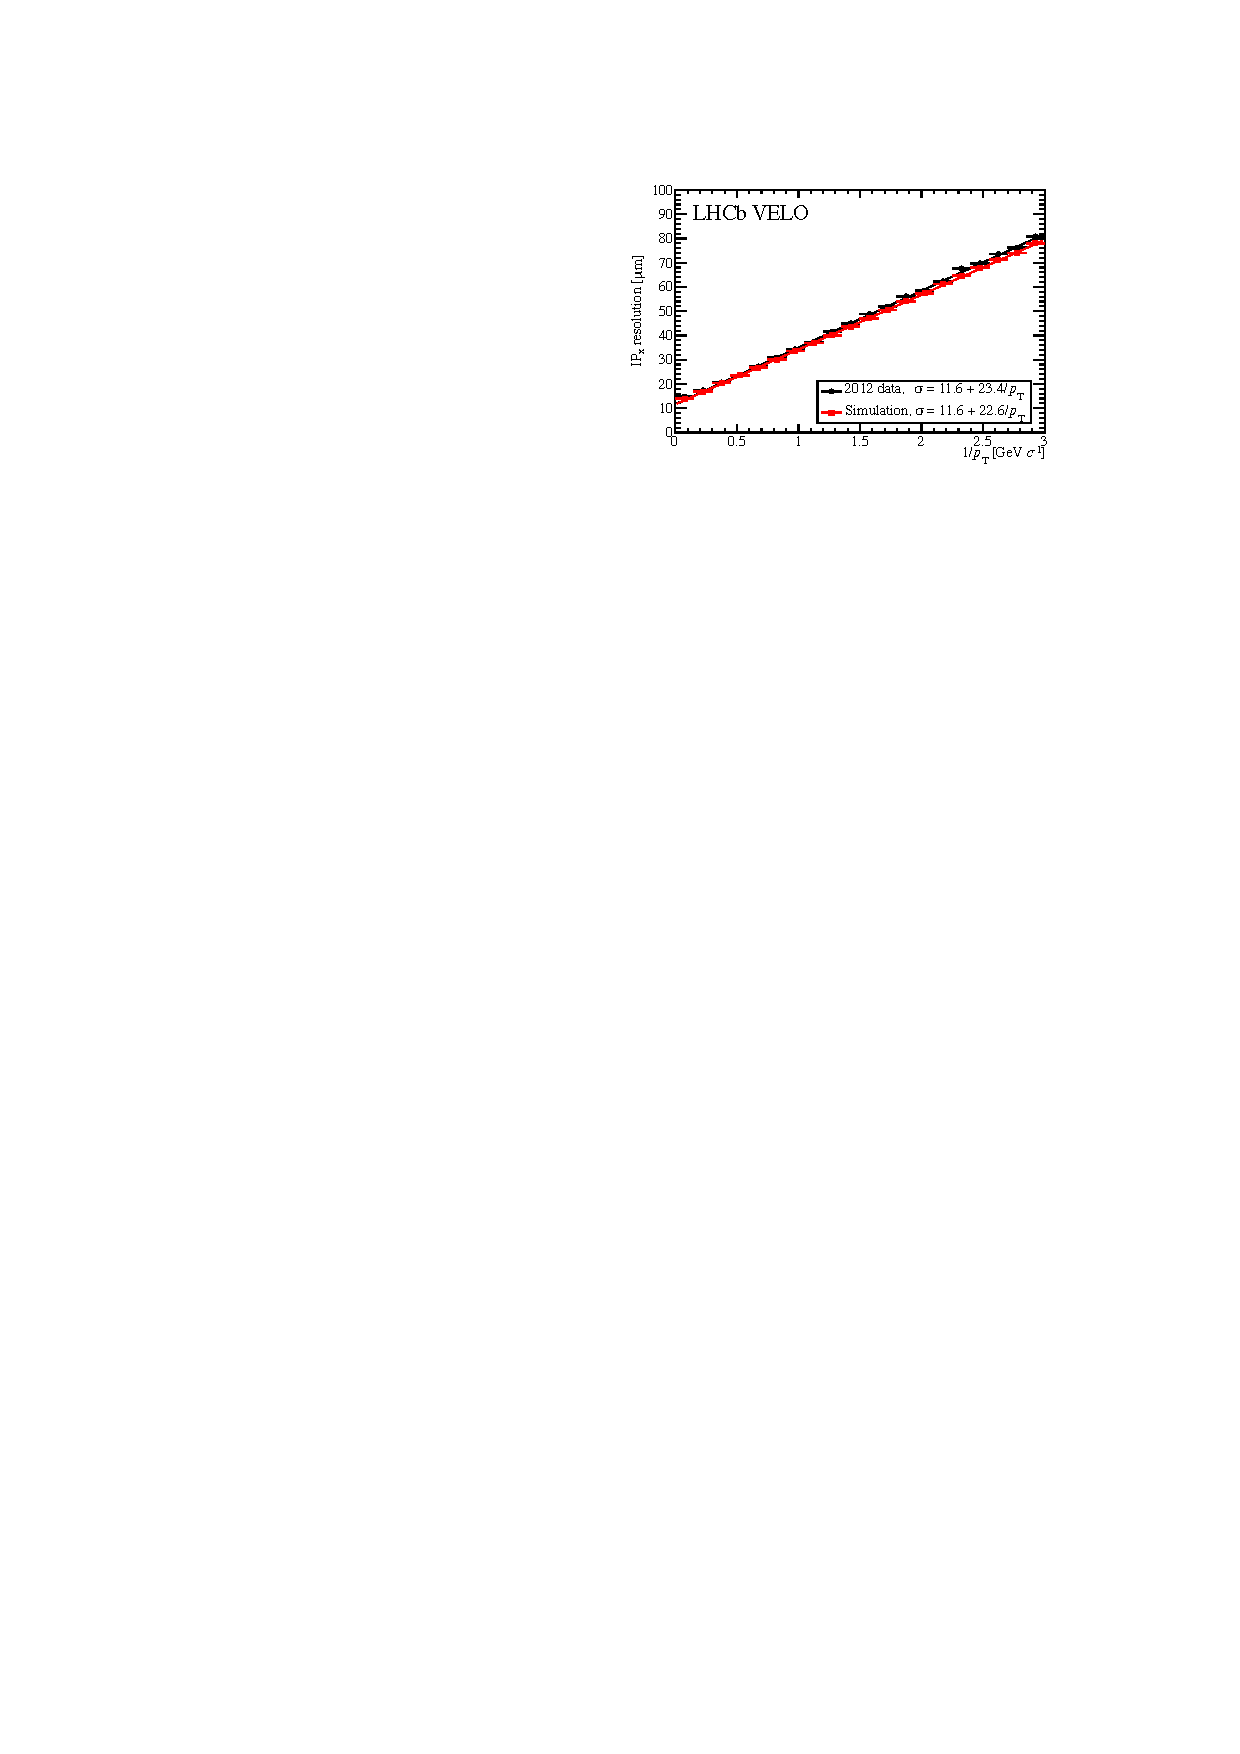
\includegraphics[width=1.0\textwidth]{figs/Detector/velo_ipx_resolution.pdf}
    \end{subfigure}
    \caption{The tracking efficiency (left) and $\text{IP}_{x}$ resolution (right) in simulation and data, from Ref.~\cite{LHCb-DP-2014-001}.}
    \label{fig:Dec_velo_track_performance}   
\end{figure}
%%%%%%%%%%%%%%%%%%%%%%%%%%%%%%%%%%%%%%%%%%%%%%%%%%%%%%%%%%

The \velo is situated in a harsh environment, therefore the components gradually degrade as exposed to more and more radiation. The damage to the silicon sensors is monitored over time to ensure the sub-detector is operational and to estimate the remaining lifetime of the sensors. In between \lhc fills current-voltage (IV) scans are performed on the silicon semiconductors, measuring the current leaking as a function of the bias voltage. The evolution of this current in Run I is shown in Fig.~\ref{fig:Dec_velo_run2_performance}, along with the delivered luminosity. These measurements help to predict what bias voltages will required by the end of Run II. 

%%%%%%%%%%%%%%%%%%%%%%%%%%%%%%%%%%%%%%%%%%%%%%%%%%%%%%%%%%
\begin{figure}[!h]
    \centering
    \begin{subfigure}[m]{0.55\textwidth}
        \centering
        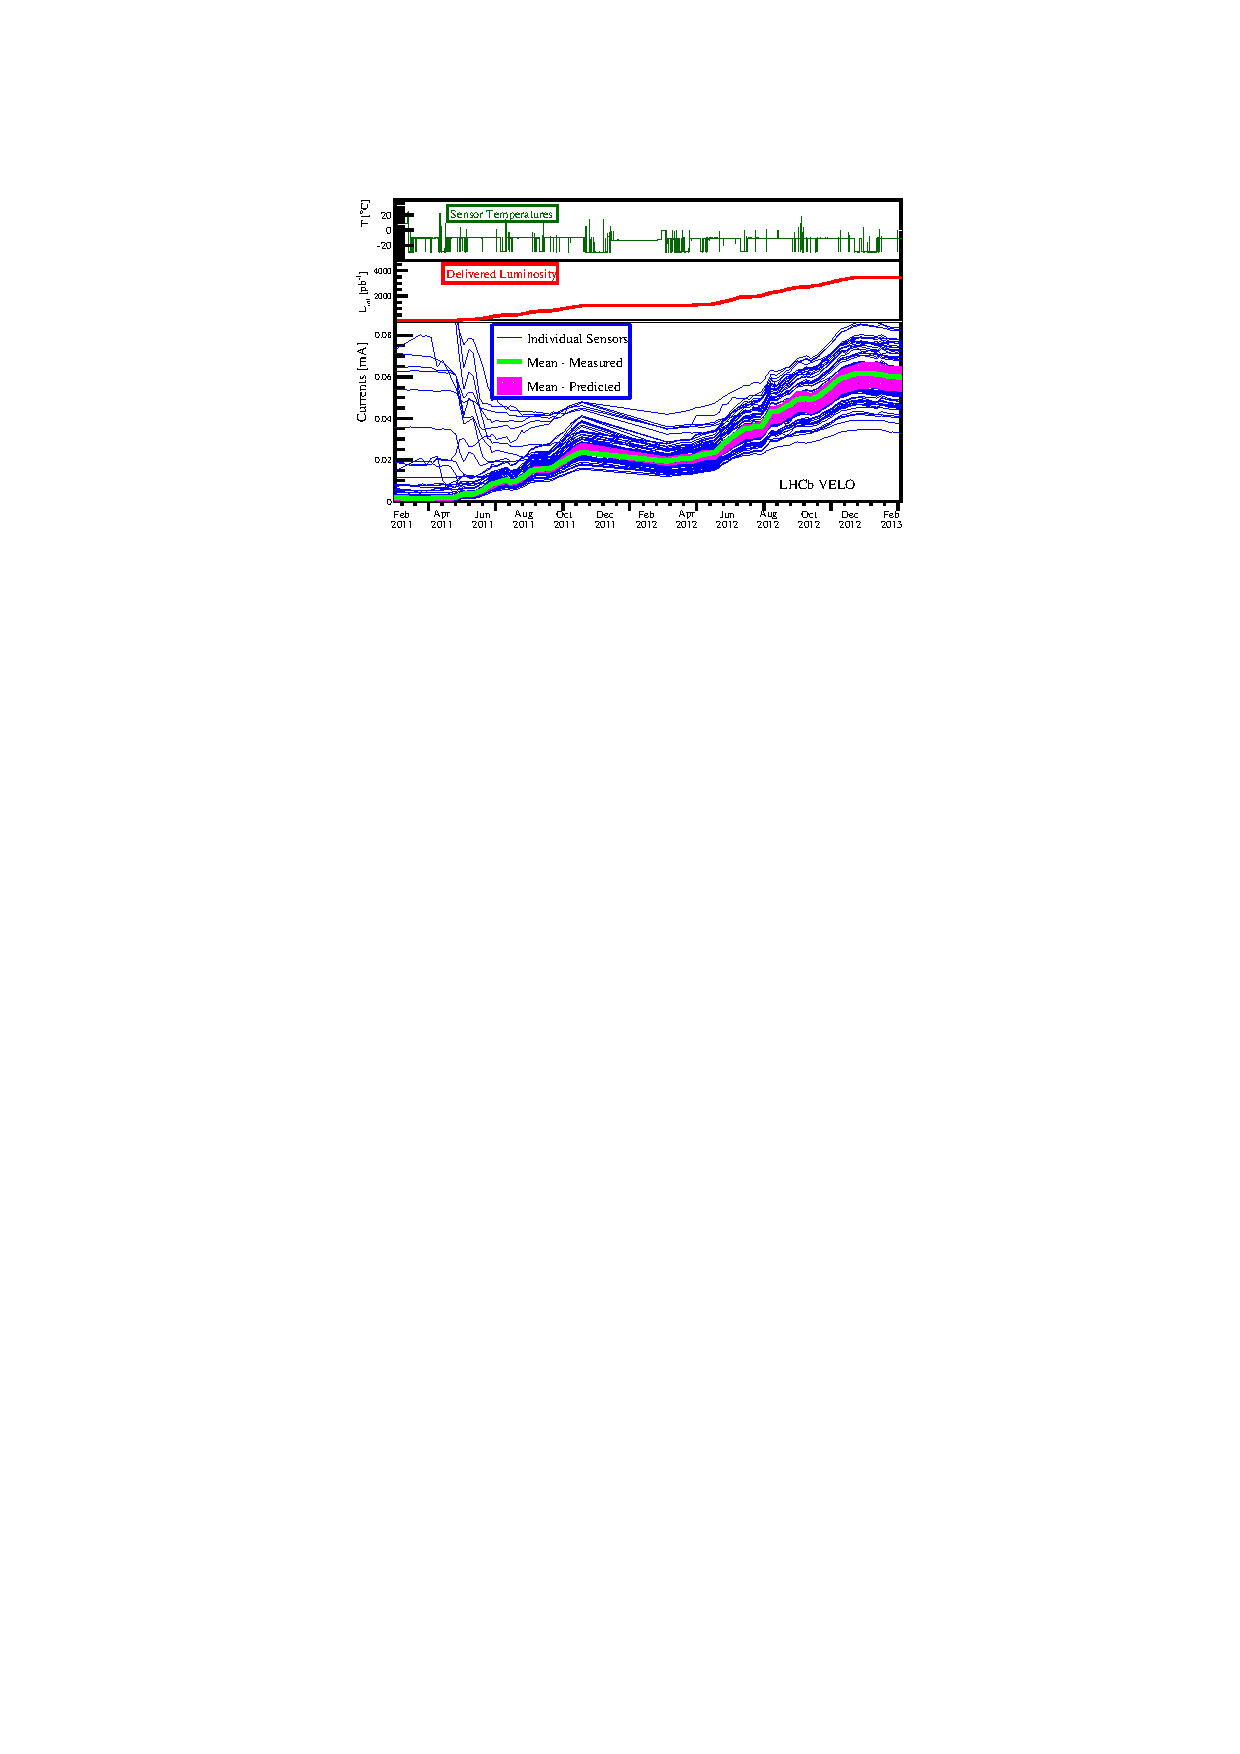
\includegraphics[width=1.0\textwidth]{figs/Detector/velo_leakage_current.pdf}
    \end{subfigure}
    \begin{subfigure}[m]{0.4\textwidth}
        \centering
        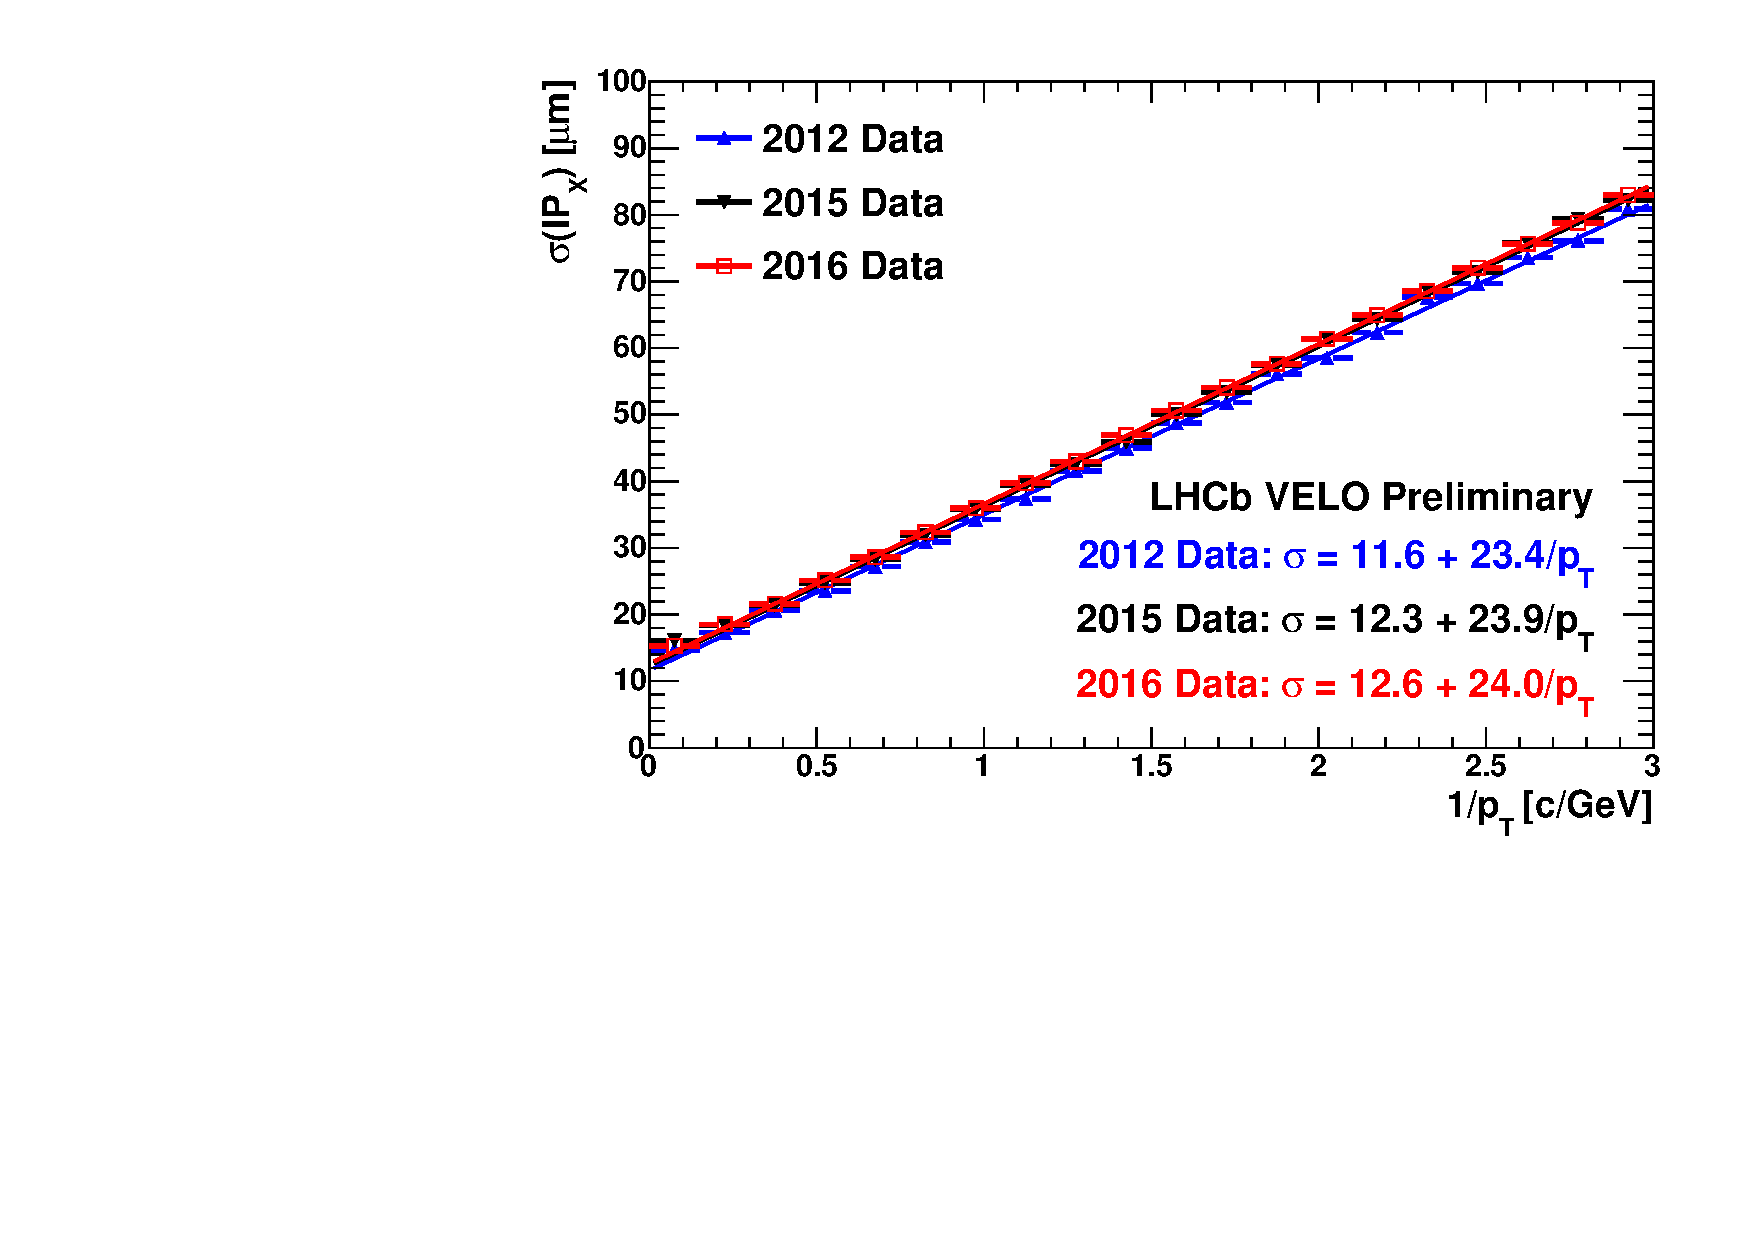
\includegraphics[width=1.0\textwidth]{figs/Detector/velo_ip_2016_2015_2012.pdf}
    \end{subfigure}
    \caption{The \velo silicon sensor's leakage current as a function of time through out Run I, from Ref.~\cite{Rinnert:2015uns} (left) and the \velo IP resolution in 2012, 2015 and 2016 data (right) . A small decrease in performance is observed between Run I and Run II.}
    \label{fig:Dec_velo_run2_performance}   
\end{figure}
%%%%%%%%%%%%%%%%%%%%%%%%%%%%%%%%%%%%%%%%%%%%%%%%%%%%%%%%%%

A comparison of the IP resolution determined using 2012, 2015 and 2016 data is also shown in Fig.~\ref{fig:Dec_velo_run2_performance}. Although the resolution is broadly similar between the three years, a slight increase in the resolution is present between Run I and Run II. 


% %%%%%%%%%%%%%%%%%%%%%%%%%%%%%%%%%%%%%%%%%%%%%%%%%%%%%%%%%%
% \begin{figure}[!h]
%     \centering
%     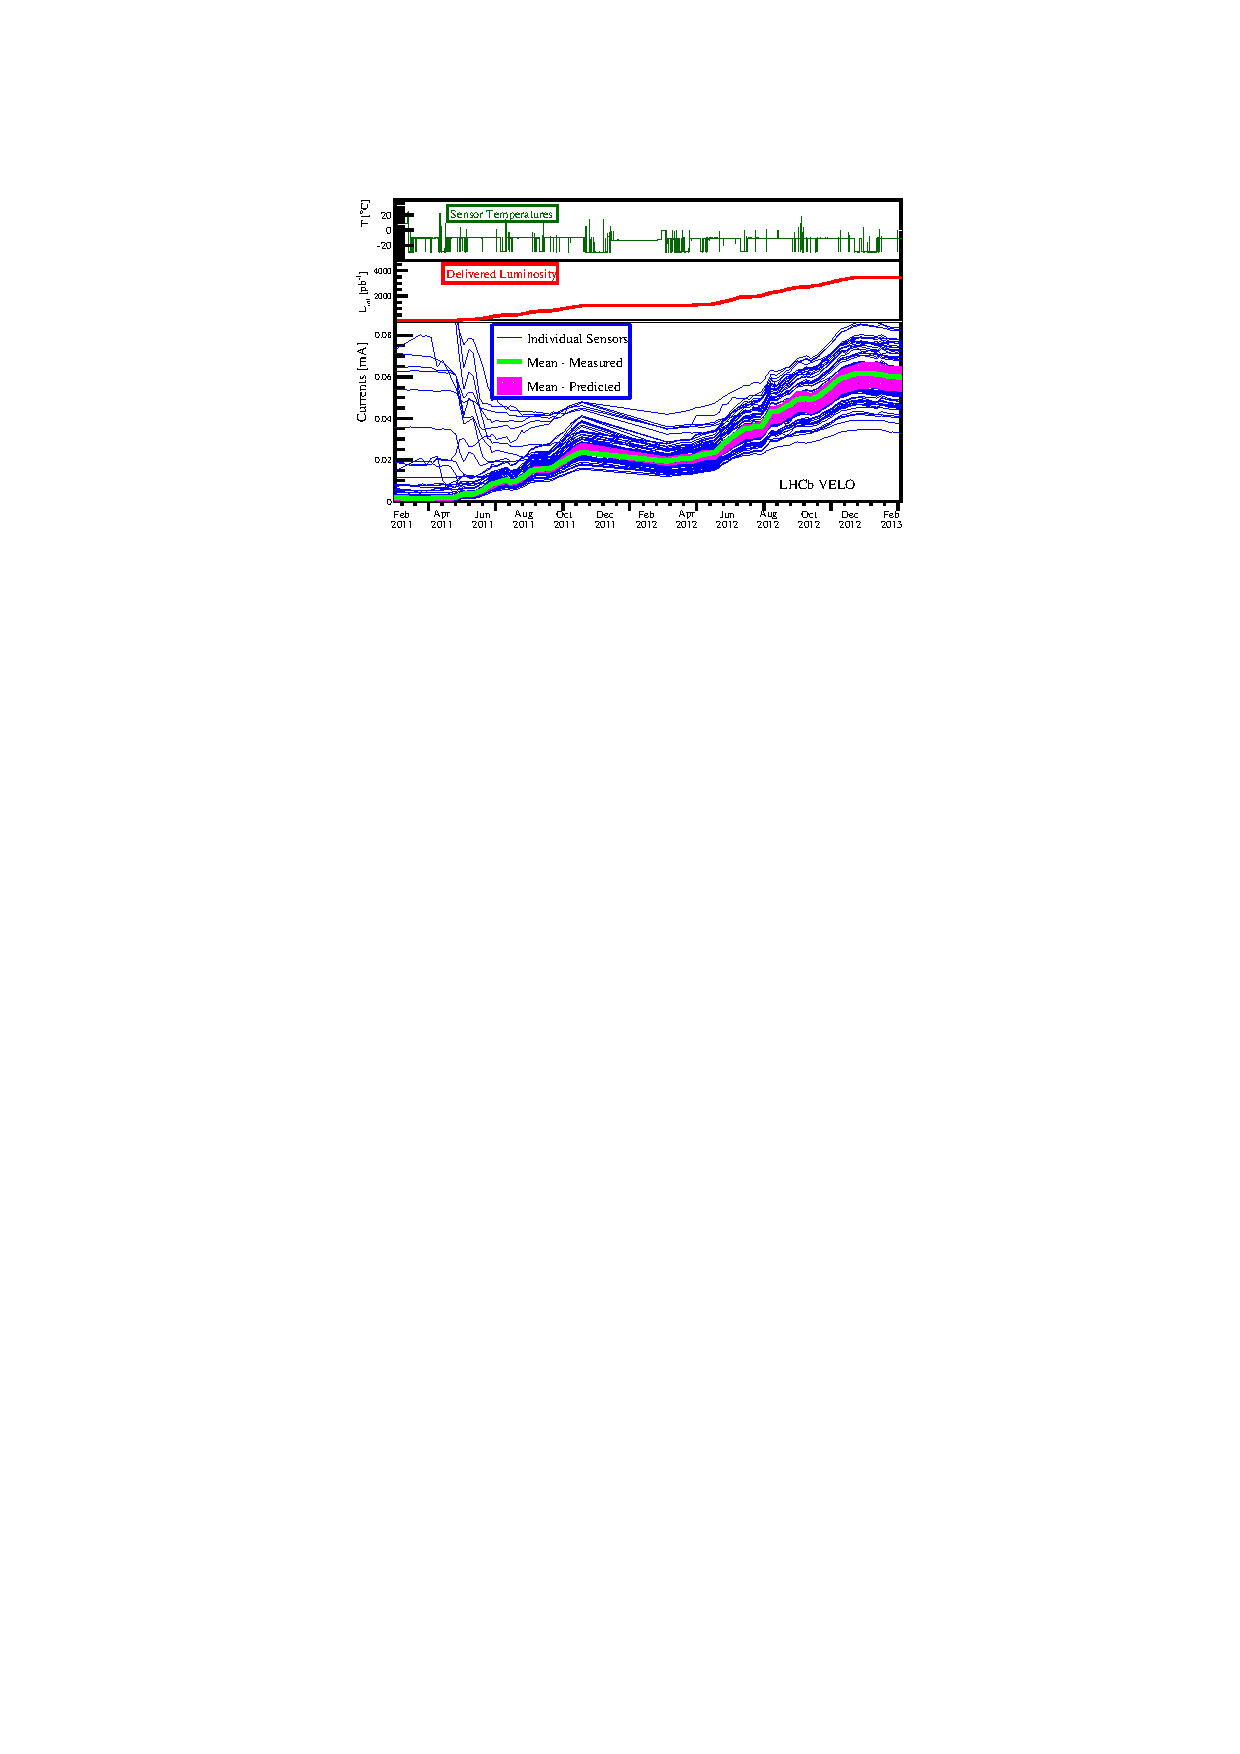
\includegraphics[width=0.6\textwidth]{figs/Detector/velo_leakage_current.pdf}
%     \caption{The \velo silicon sensor's leakage current as a function of time through out Run I, from Ref.~\cite{Rinnert:2015uns}.}
%     \label{fig:Dec_velo_leakage_current}   
% \end{figure}
% %%%%%%%%%%%%%%%%%%%%%%%%%%%%%%%%%%%%%%%%%%%%%%%%%%%%%%%%%%




% %%%%%%%%%%%%%%%%%%%%%%%%%%%%%%%%%%%%%%%%%%%%%%%%%%%%%%%%%%
% \begin{figure}[!h]
%     \centering
%     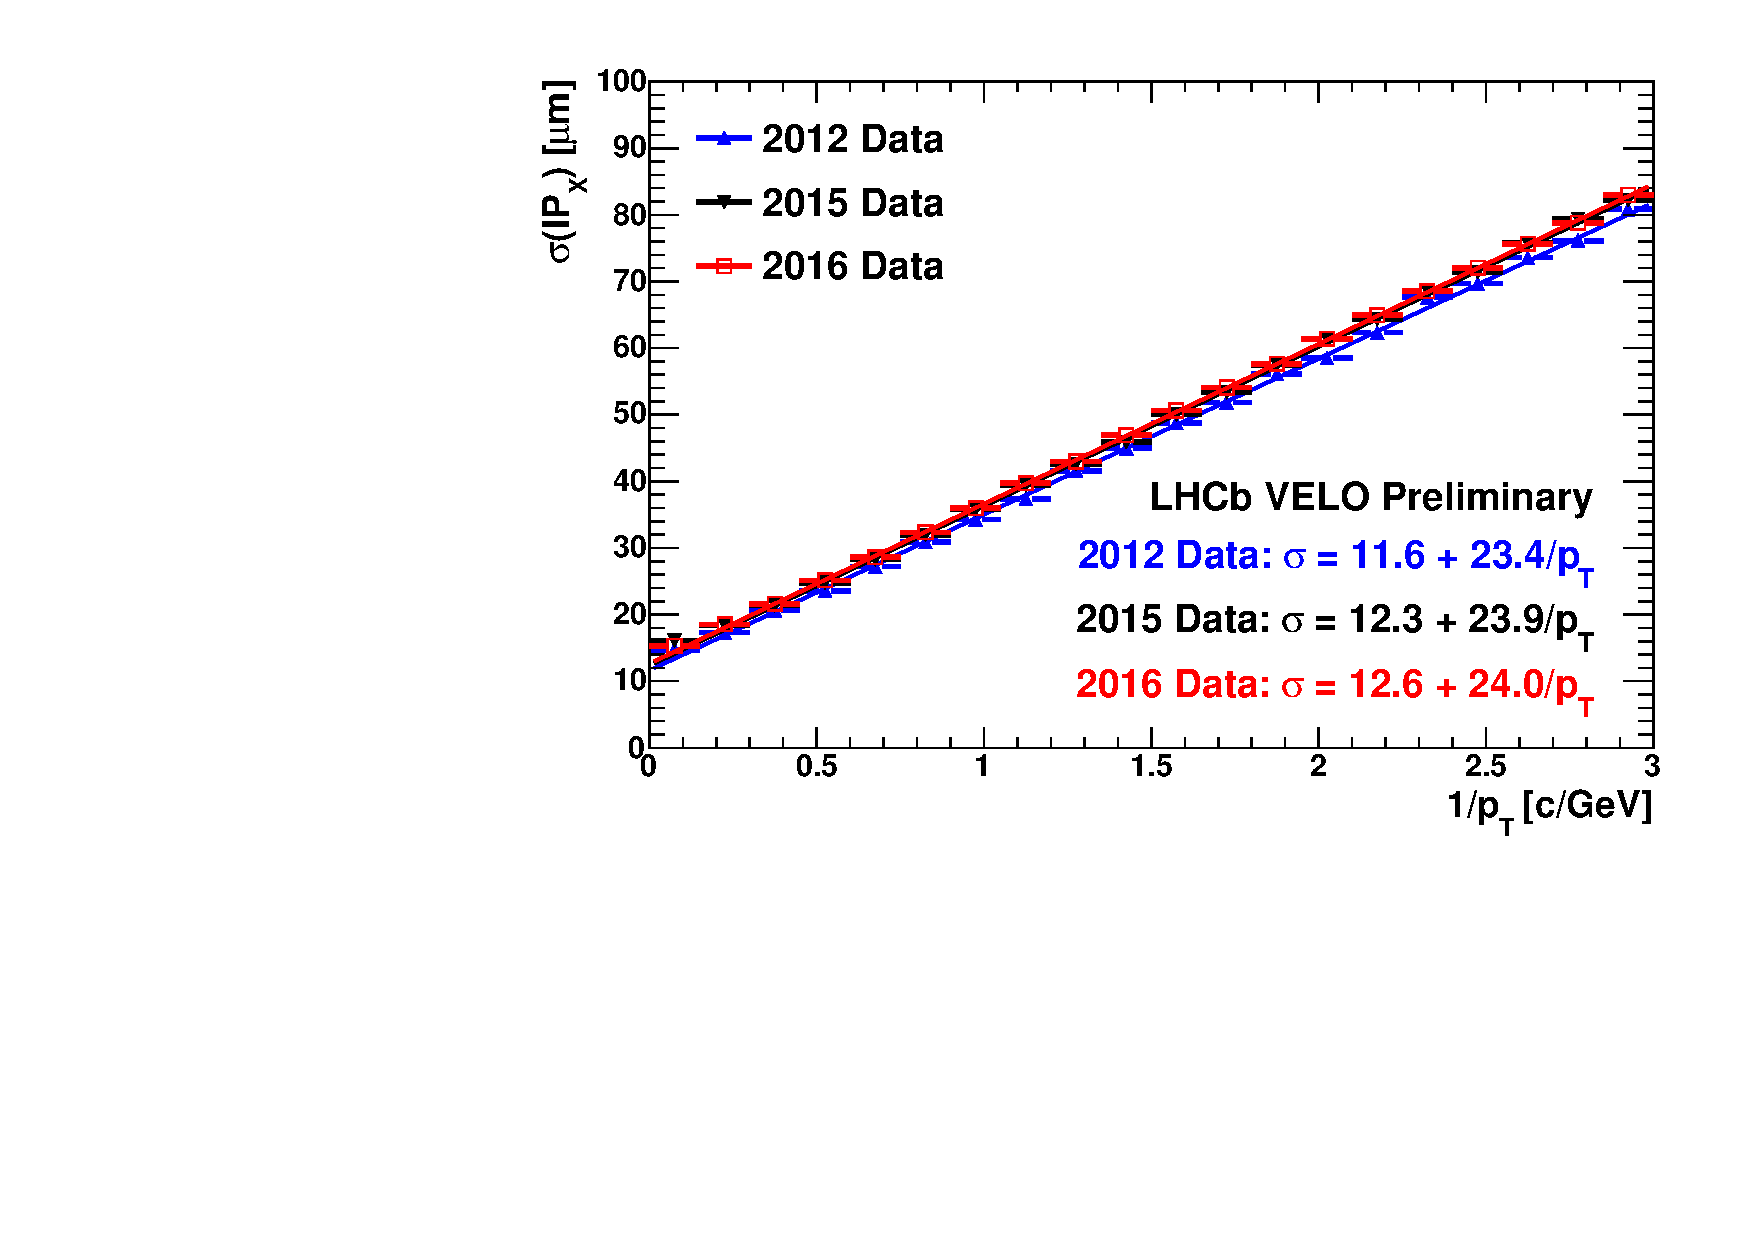
\includegraphics[width=0.4\textwidth]{figs/Detector/velo_ip_2016_2015_2012.pdf}
%     \caption{The \velo IP resolution in 2012, 2015 and 2016 data. A small decrease in performance is observed between Run I and Run II.}
%     \label{fig:Dec_velo_run1_run2_comparison}   
% \end{figure}
% %%%%%%%%%%%%%%%%%%%%%%%%%%%%%%%%%%%%%%%%%%%%%%%%%%%%%%%%%%



\subsection{Silicon Tracker}

In addition to the \velo, there are two more sub-detectors that utilise silicon sensors in order to determine tracking information. These are collectively referred to as the Silicon Tracker (\st), which is made up of two trackers; the Tracker Turicensis (\ttracker) and Inner Tracker (\intr). The \ttracker is located before the dipole magnet, whereas the \intr is positioned after, as show in Fig.~\ref{fig:Dec_lhcb_Schematic}. Although these two detectors are spatially separated, their common silicon mircostrip sensors and electronics warrant considering them together.

The silicon sensors are made up of single-sided $p^{+}$-on-$n$ sensors. The hits are read out via chips at the end of each module. These chips are the same custom analogue chips used in the \velo sub-detector. The signals pass into digitisers and then through optical fibres into \tellone boards that perform clustering algorithms.
Both sub-detectors are cooled to 5\degrees{C} and their sealed containers flushed with nitrogen gas to prevent condensation.



\subsubsection{Tracker Turicensis}

The \ttracker is positioned before the dipole magnet and covers the entire \lhcb acceptance, standing 130\cm tall and 150\cm wide.
It is made up of four layers orientated at angles to one another. The first and fourth layers are parallel, with the second and third at angles -5\degrees and +5\degrees to these respectively. The first and second are separated from the third and fourth by 27\cm along the beam axis. The layout of the silicon modules in the \ttracker is shown in Fig.~\ref{fig:Dec_tt_scematic}. The sensors are grouped into \emph{half-modules} that span half of the vertical height of the sub-detector. These are made up of seven silicon sensors and a readout hybrid at the outermost end. The readout electronics are positioned outside of the \lhcb acceptance, limiting the amount of multiple scattering due to interactions with the detector material. 

The \emph{half-modules} are arranged to prevent any gaps in the instrumentation. The adjacent \emph{half-modules} are offset by 1\cm along the beam axis, allowing the modules to overlap by a few millimetres in the $x$-axis. 


%%%%%%%%%%%%%%%%%%%%%%%%%%%%%%%%%%%%%%%%%%%%%%%%%%%%%%%%%%
\begin{figure}[!h]
    \centering
    \begin{subfigure}[m]{0.49\textwidth}
        \centering
        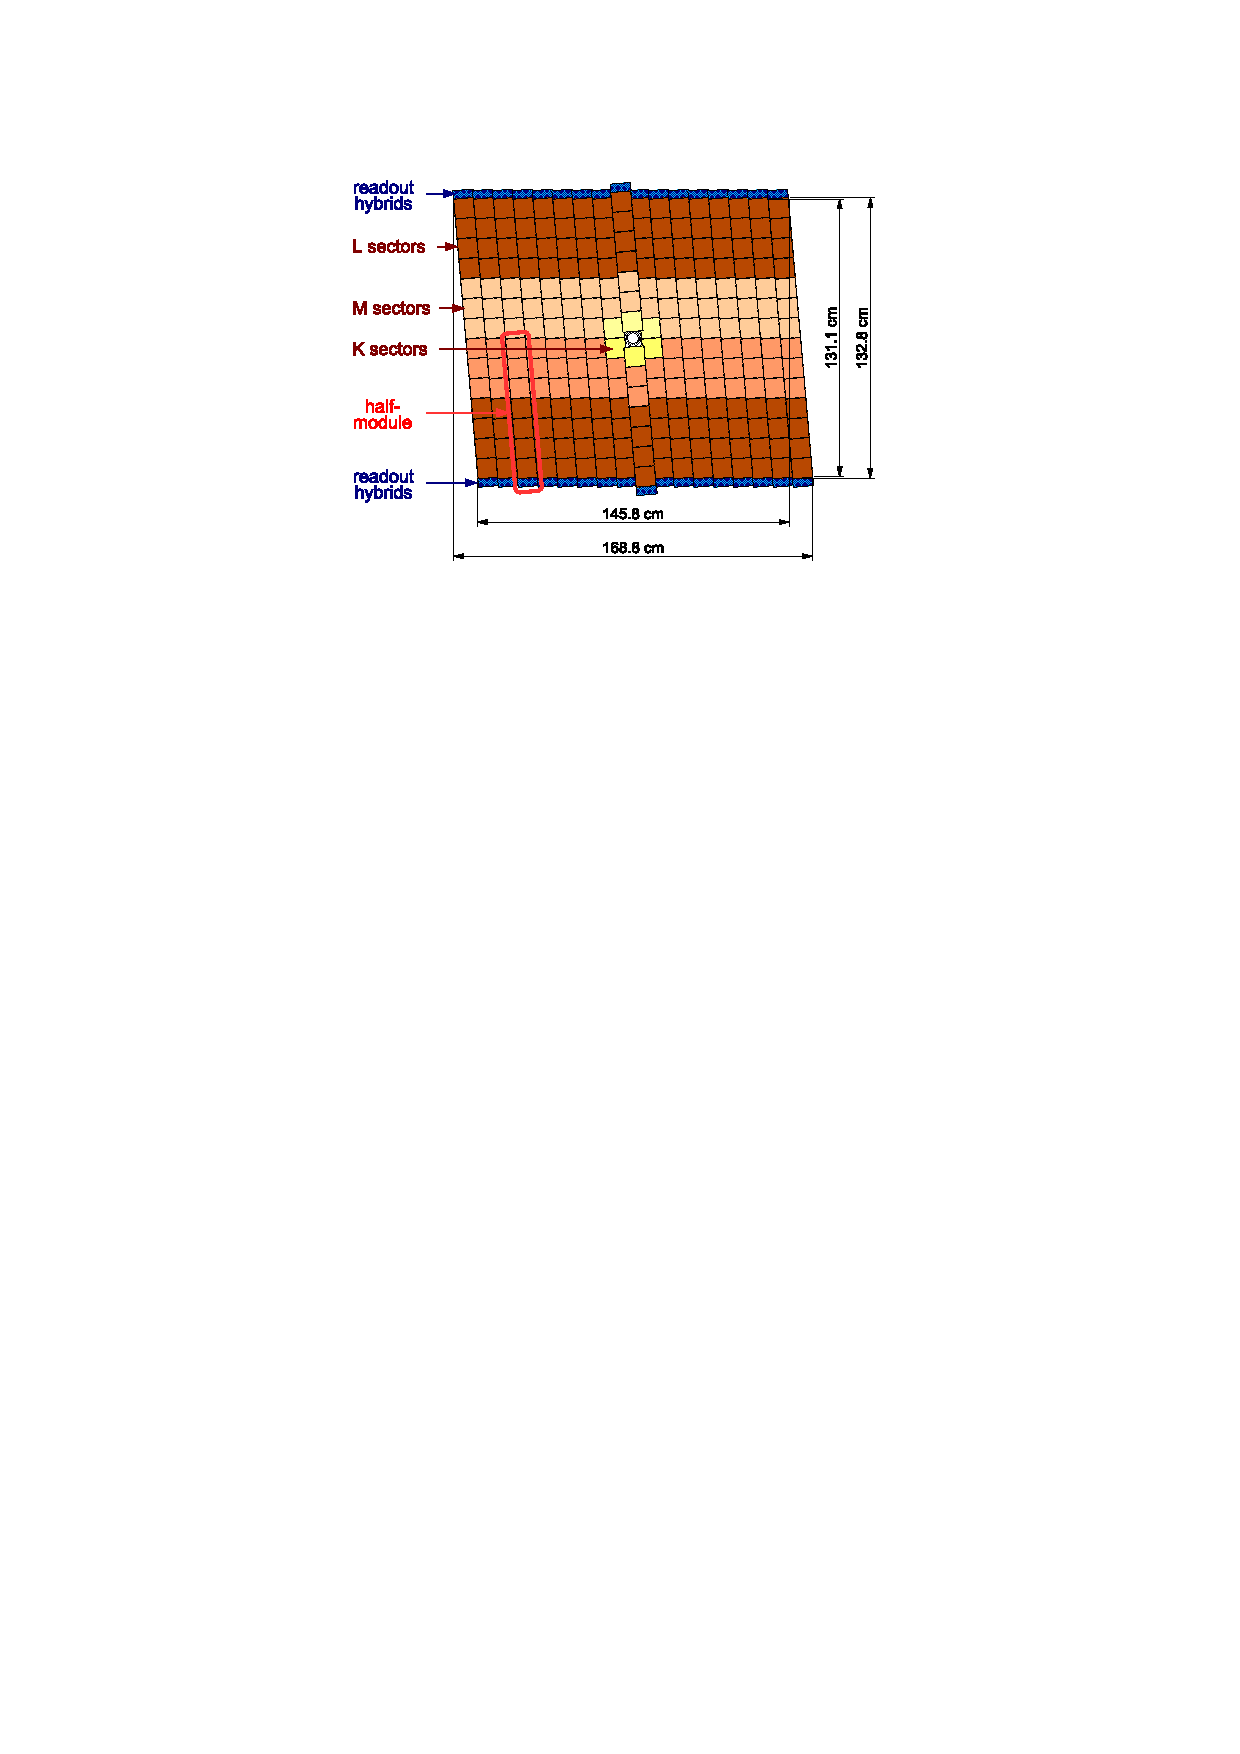
\includegraphics[width=1.0\textwidth]{figs/Detector/tt_layout.pdf}
    \end{subfigure}
    \begin{subfigure}[m]{0.49\textwidth}
        \centering
        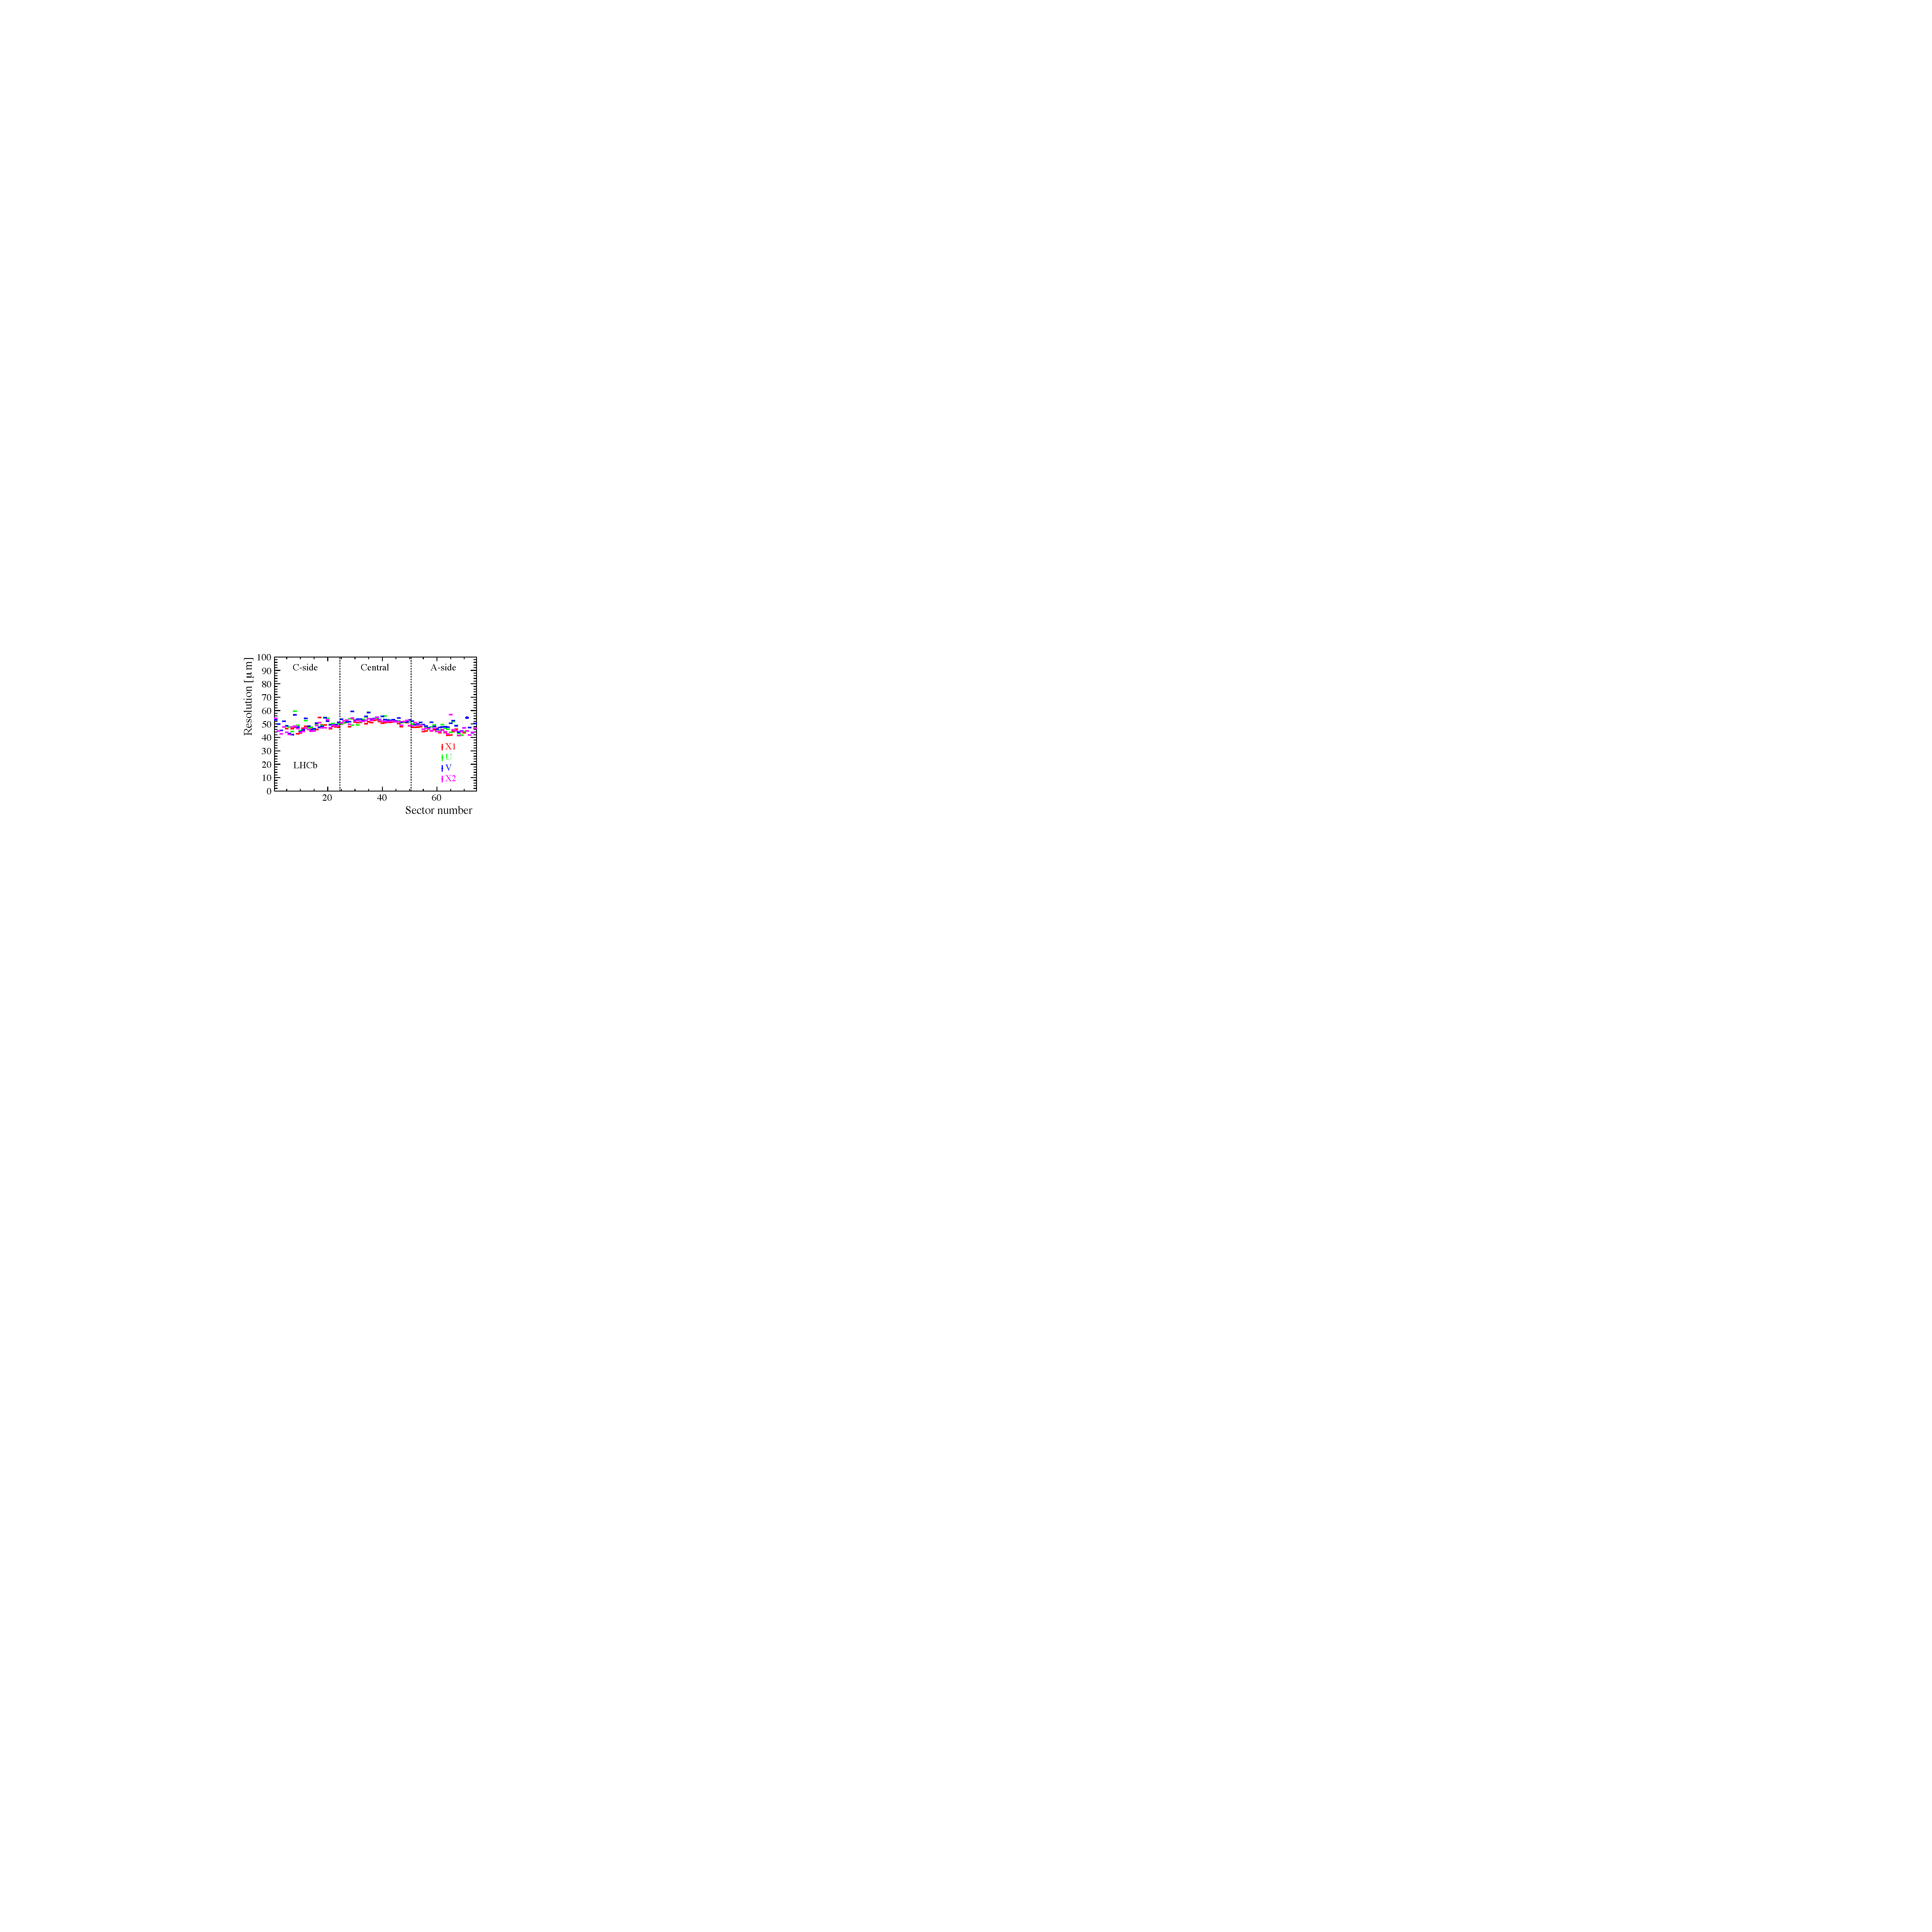
\includegraphics[width=1.0\textwidth]{figs/Detector/tt_resolution.pdf}
    \end{subfigure}
    \caption{Schematic of the \ttracker sub-detector, from Ref.~\cite{Alves:2008zz} (left) and the \ttracker resolution by sector number, from Ref.~\cite{LHCb-DP-2014-002}.}
    \label{fig:Dec_tt_scematic}   
\end{figure}
%%%%%%%%%%%%%%%%%%%%%%%%%%%%%%%%%%%%%%%%%%%%%%%%%%%%%%%%%%


The resolution achieved by the \ttracker is shown in Fig.~\ref{fig:Dec_tt_scematic}, split into different sectors and shown separately for the four layers (labelled X1, U , V and X2). The resolution vary between 40--60\mum and is consistent between the different layers. 


\subsubsection{Inner Tracker}

The \intr is the second silicon detector making up the \st. It is located after the dipole magnet in three tracking stations. As the name implies, it covers only the inner region of the acceptance, measuring 140\cm wide and 40\cm tall, where the particle flux is highest. The rest of the area is covered by the much larger Outer Tracker. Similar to the \ttracker, the \intr is made up of four layers positioned at slight angles to one another. However, as shown in Fig.~\ref{fig:Dec_lhcb_Schematic}, there are three separate \intr stations, each containing four layers.
These stations are constructed as of four boxes distributed around the beam-pipe in a cross shape, as shown in Fig.~\ref{fig:Dec_it_scematic}. 



%%%%%%%%%%%%%%%%%%%%%%%%%%%%%%%%%%%%%%%%%%%%%%%%%%%%%%%%%%
\begin{figure}[!h]
    \centering
    \begin{subfigure}[m]{0.49\textwidth}
        \centering
        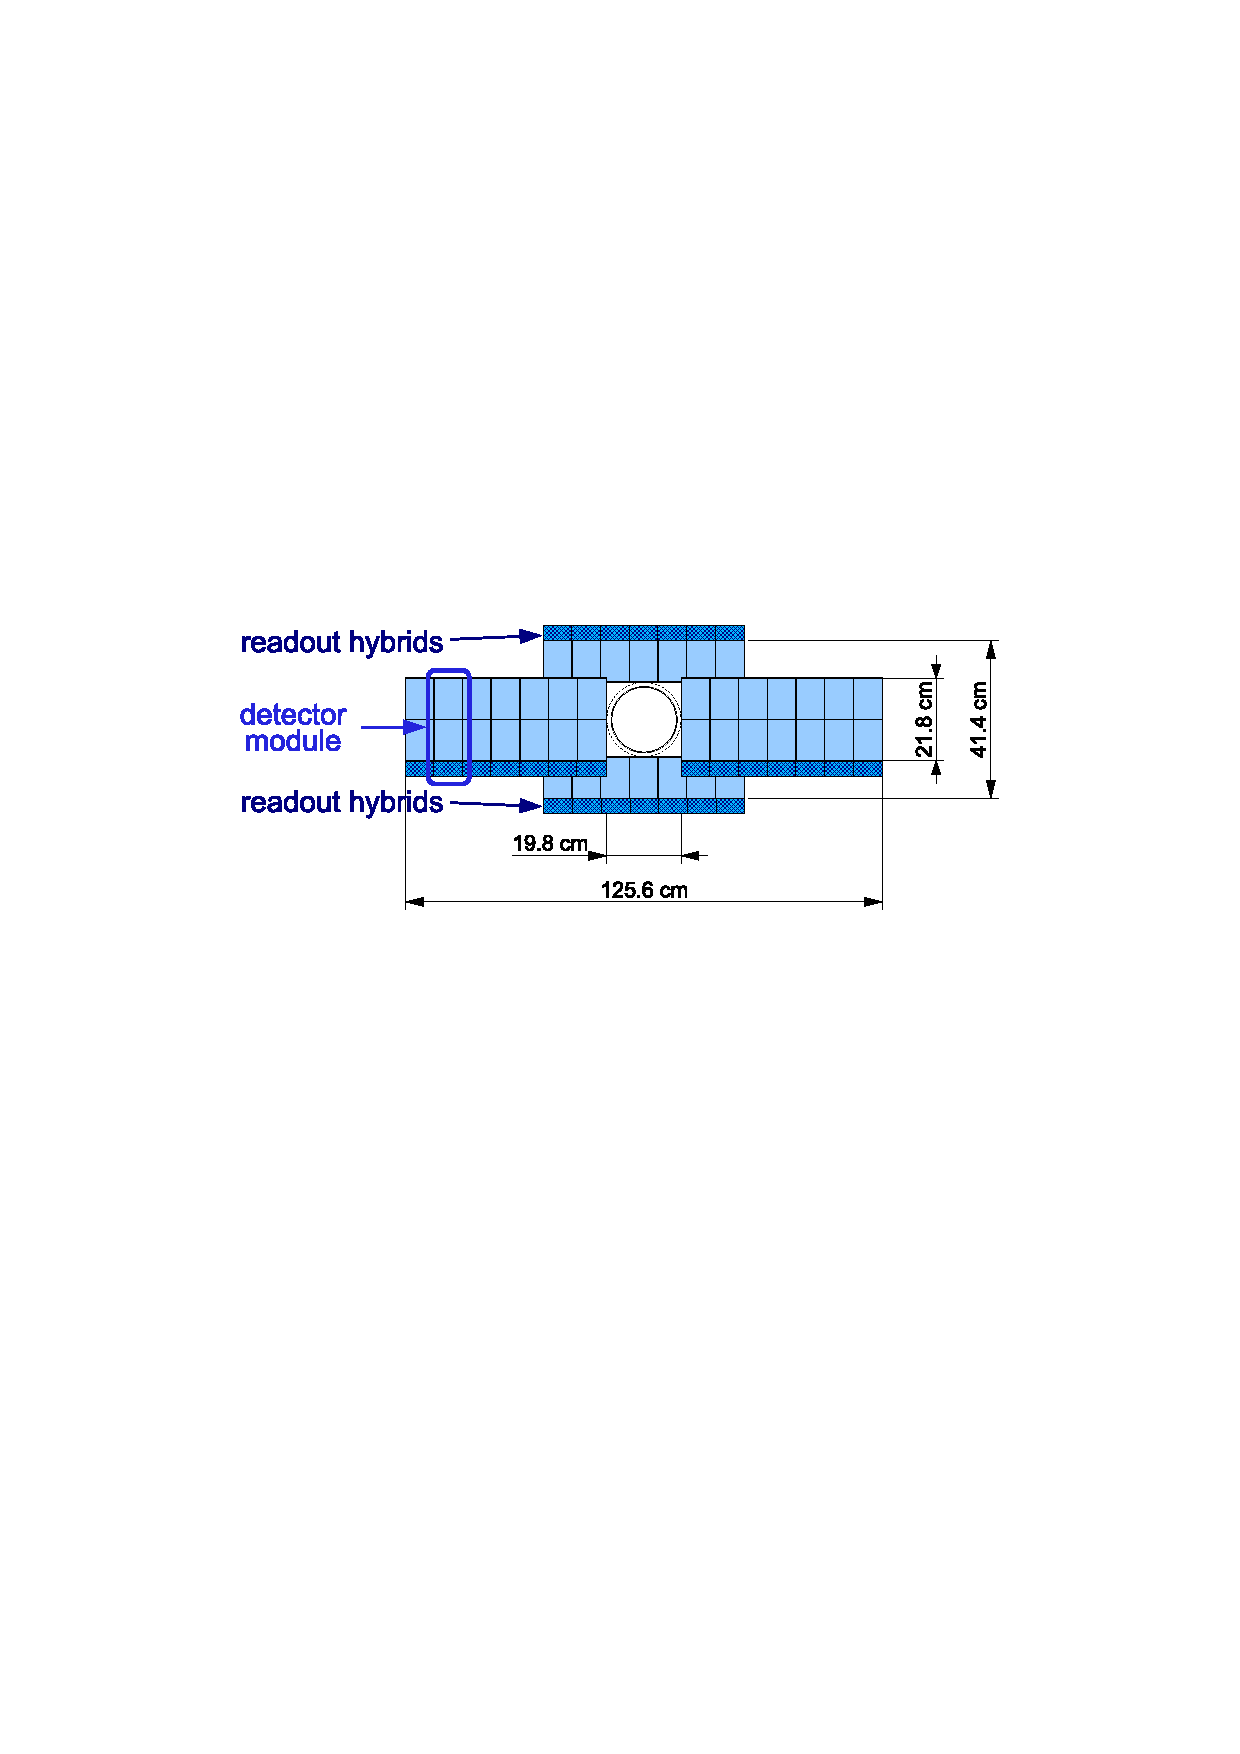
\includegraphics[width=1.0\textwidth]{figs/Detector/it_layout.pdf}
    \end{subfigure}
    \begin{subfigure}[m]{0.49\textwidth}
        \centering
        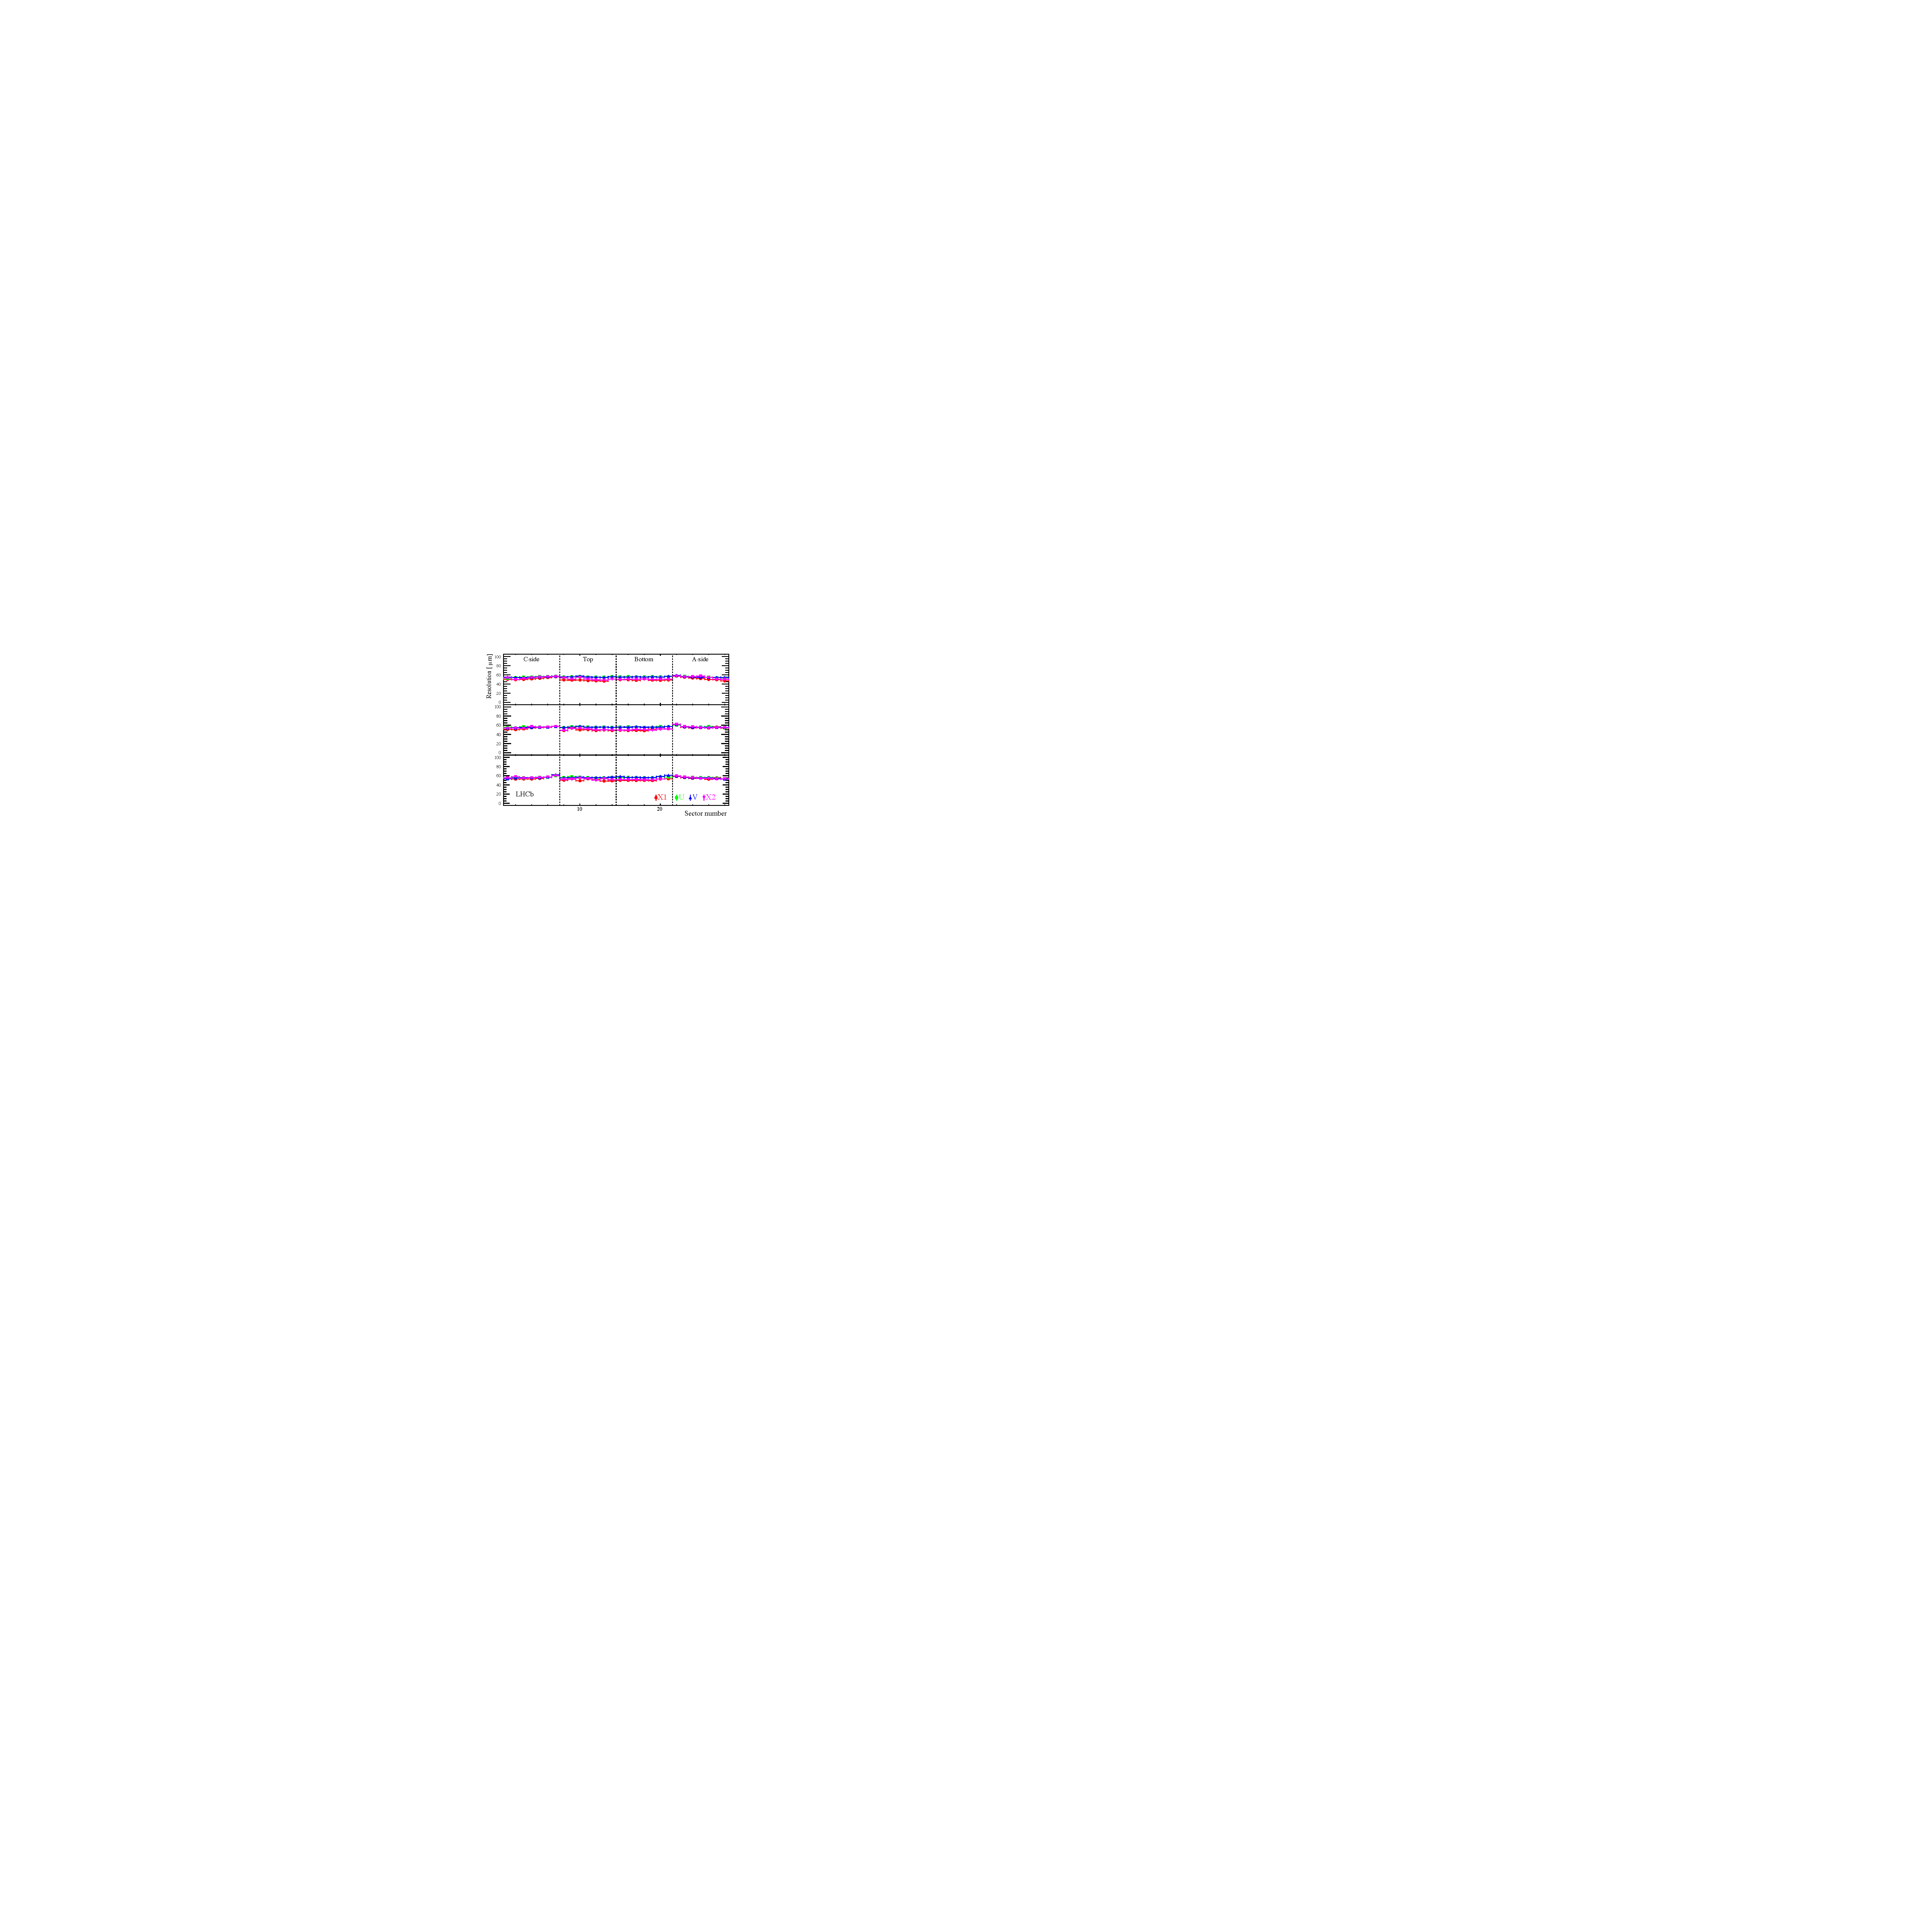
\includegraphics[width=1.0\textwidth]{figs/Detector/it_resolution.pdf}
    \end{subfigure}
    \caption{Schematic of the \intr sub-detector, from Ref.~\cite{Alves:2008zz} (left) and the \intr resolution by sector number, from Ref.~\cite{LHCb-DP-2014-002}.}
    \label{fig:Dec_it_scematic}   
\end{figure}
%%%%%%%%%%%%%%%%%%%%%%%%%%%%%%%%%%%%%%%%%%%%%%%%%%%%%%%%%%



The detector modules consist of either one or two silicon sensors and a readout chip. These are also offset along the beam axis to allow the modules to overlap slightly in the $x$-axis.

The resolution of the \intr is shown in Fig.~\ref{fig:Dec_it_scematic}. The resolution is between 40--60\mum and varies between the four different layers.    



\subsection{Outer Tracker}

In contrast to the the silicon-based sub-detectors already described, the Outer Tracker (\ot) is a straw tube tracker filled with a gaseous mixture of argon, carbon dioxide and oxygen. The 4.9\mm diameter straws are 2.4\m in length and arranged in double layers as shown in Fig.~\ref{fig:Dec_ot_schematic}. As with the \intr, the \ot is split into three stations. Each of these stations similarly has four layers arranged at angles to one another $(0\degrees,-5\degrees,+5\degrees,0\degrees)$. The arrangement of the stations and layers are also shown in Fig.~\ref{fig:Dec_ot_schematic}. The inner region occupied by the \intr is visible.

%%%%%%%%%%%%%%%%%%%%%%%%%%%%%%%%%%%%%%%%%%%%%%%%%%%%%%%%%%
\begin{figure}[!h]
    \centering
    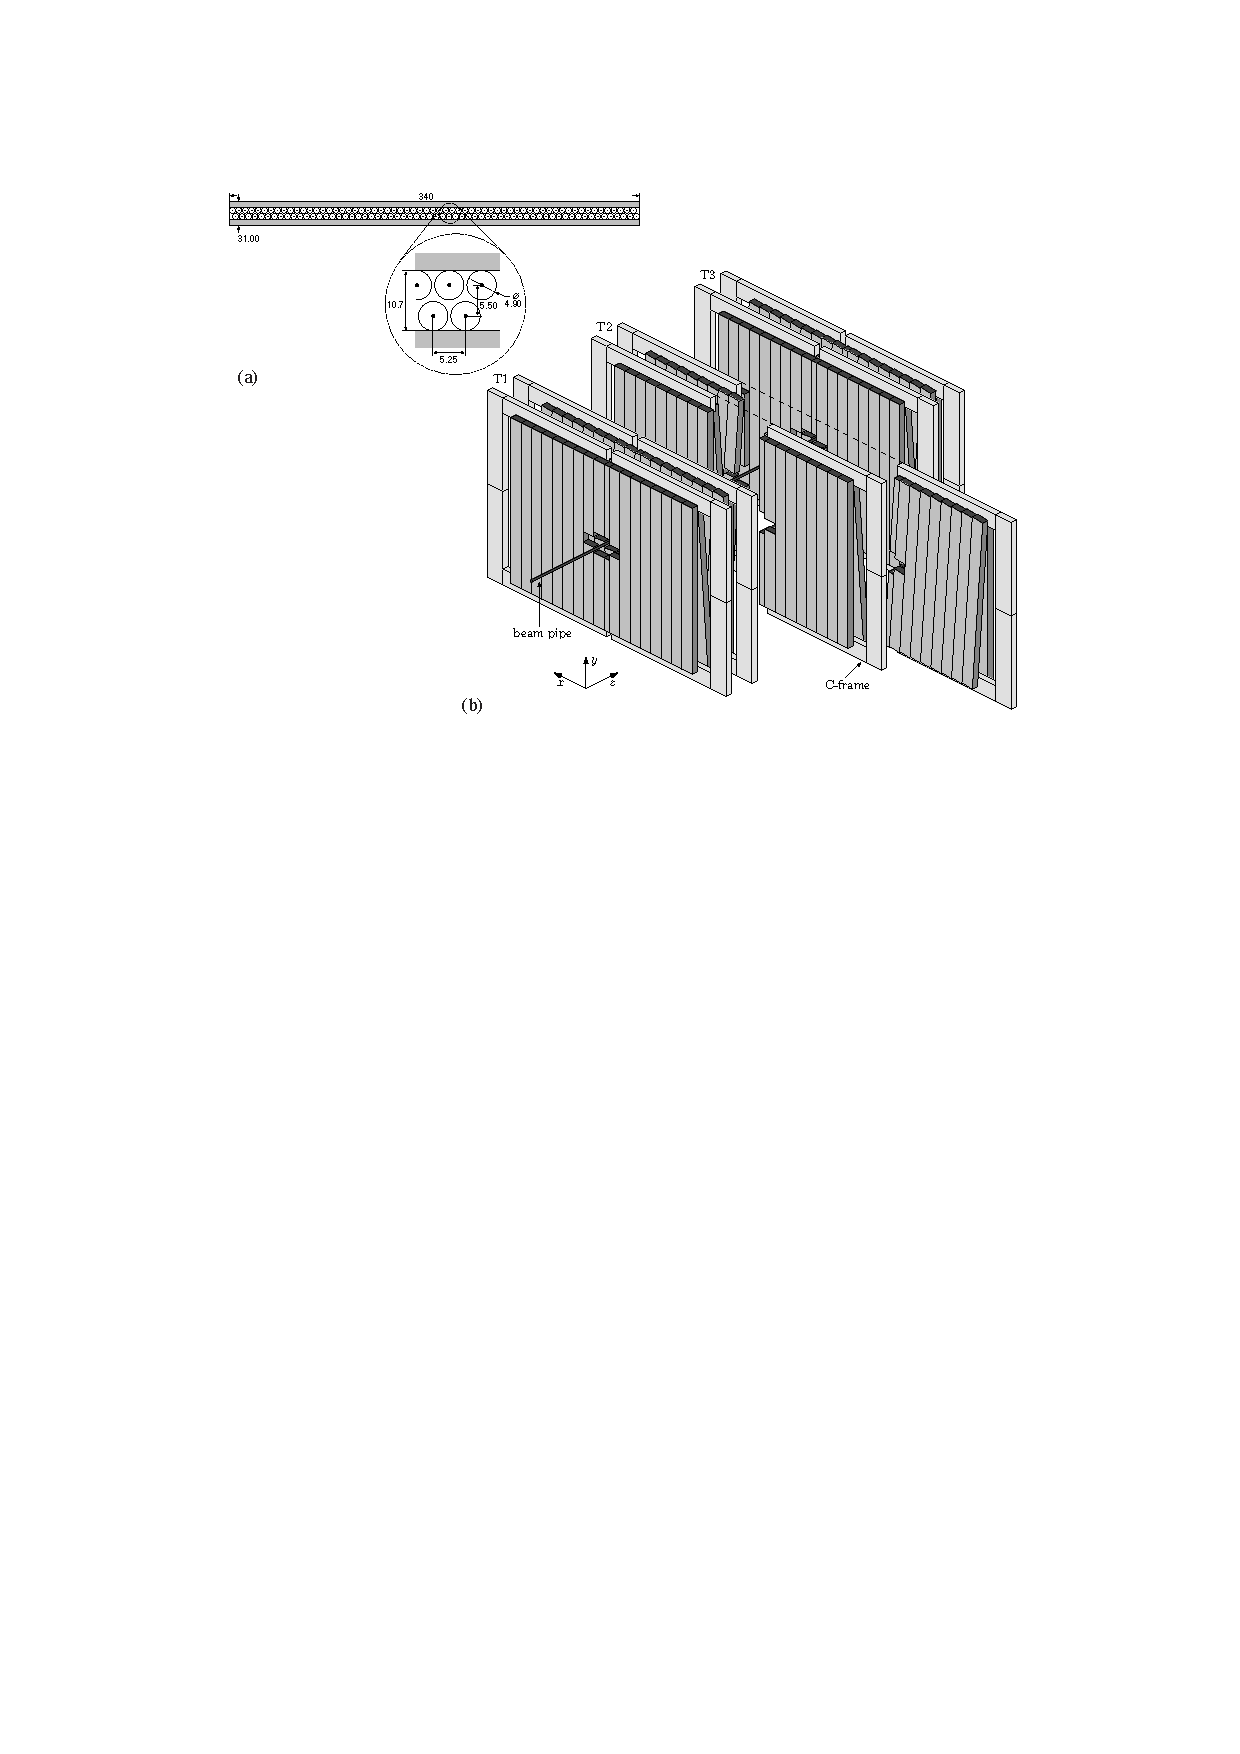
\includegraphics[width=0.8\textwidth]{figs/Detector/ot_layout.pdf}
    \caption{Schematic of the \ot sub-detector, from Ref.~\cite{LHCb-DP-2013-003}.}
    \label{fig:Dec_ot_schematic}   
\end{figure}
%%%%%%%%%%%%%%%%%%%%%%%%%%%%%%%%%%%%%%%%%%%%%%%%%%%%%%%%%%
 
The straws comprising the tracker are composed of an inner wire surrounded by a conducting foil, with a potential difference maintained between the two. When a charged particle passes through the straw the gas becomes ionised. The electrons and gas ions are attracted to the cathode foil and anode wire, resulting in a flow of current. In the \ot the inner wire is made of 25\mum thick gold plated tungsten and maintained at a voltage of +1550\,V. The surrounding foil is made up of three layers; a 40\mum thick layer of conducting carbon-doped polyimide film; a 12.5\mum layer of insulating polyimide; and 12.5\mum of aluminium. 

The double layers of straw tubes as shown in Fig.~\ref{fig:Dec_ot_schematic} make up a module. Vertically, the modules are split in two, with staggered gaps between the two individual straw layers to avoid an uninstrumented region. Each of the modules are read out from the outermost end. 
The readout boards contain a number of circuits to process the signals and provide the potential difference to the straw wires.
The analogue signals pass through an amplification circuit before being are processed and cleaned. These then pass into a digitiser creating a digital value of the drift-time.   

The single hit resolution is determined for the \ot by determining the width of the hit distance residual distribution. This is shown in Fig.~\ref{fig:Dec_ot_resolution} giving a resolution of 205\mum.



%%%%%%%%%%%%%%%%%%%%%%%%%%%%%%%%%%%%%%%%%%%%%%%%%%%%%%%%%%
\begin{figure}[!h]
    \centering
    \begin{subfigure}[t]{0.4\textwidth}
        \centering
        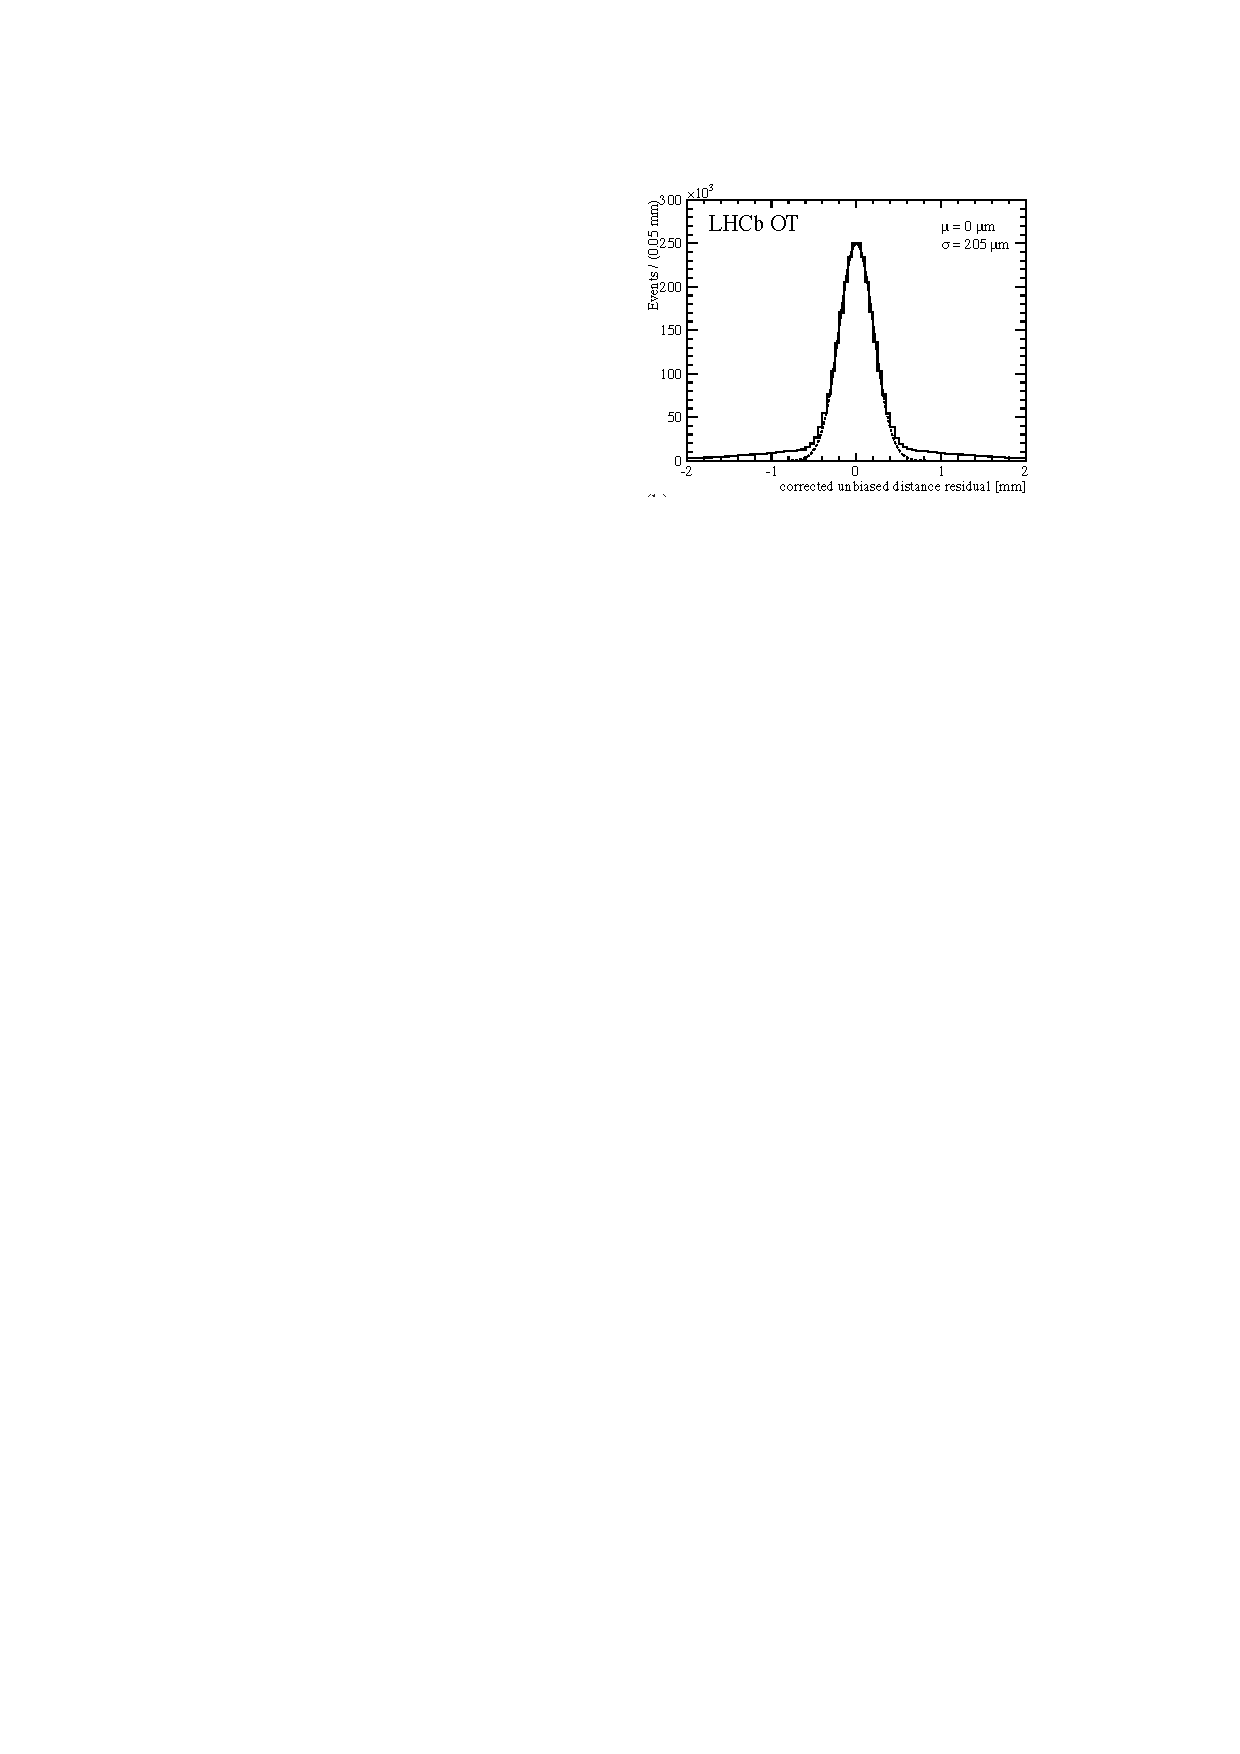
\includegraphics[width=1.0\textwidth]{figs/Detector/ot_residuals.pdf}
    \end{subfigure}
    \caption{The hit distance residuals for the \ot, from Ref.~\cite{LHCb-DP-2013-003}.}
    \label{fig:Dec_ot_resolution}   
\end{figure}
%%%%%%%%%%%%%%%%%%%%%%%%%%%%%%%%%%%%%%%%%%%%%%%%%%%%%%%%%%




% %%%%%%%%%%%%%%%%%%%%%%%%%%%%%%%%%%%%%%%%%%%%%%%%%%%%%%%%%%
% \begin{figure}[!h]
%     \centering
%     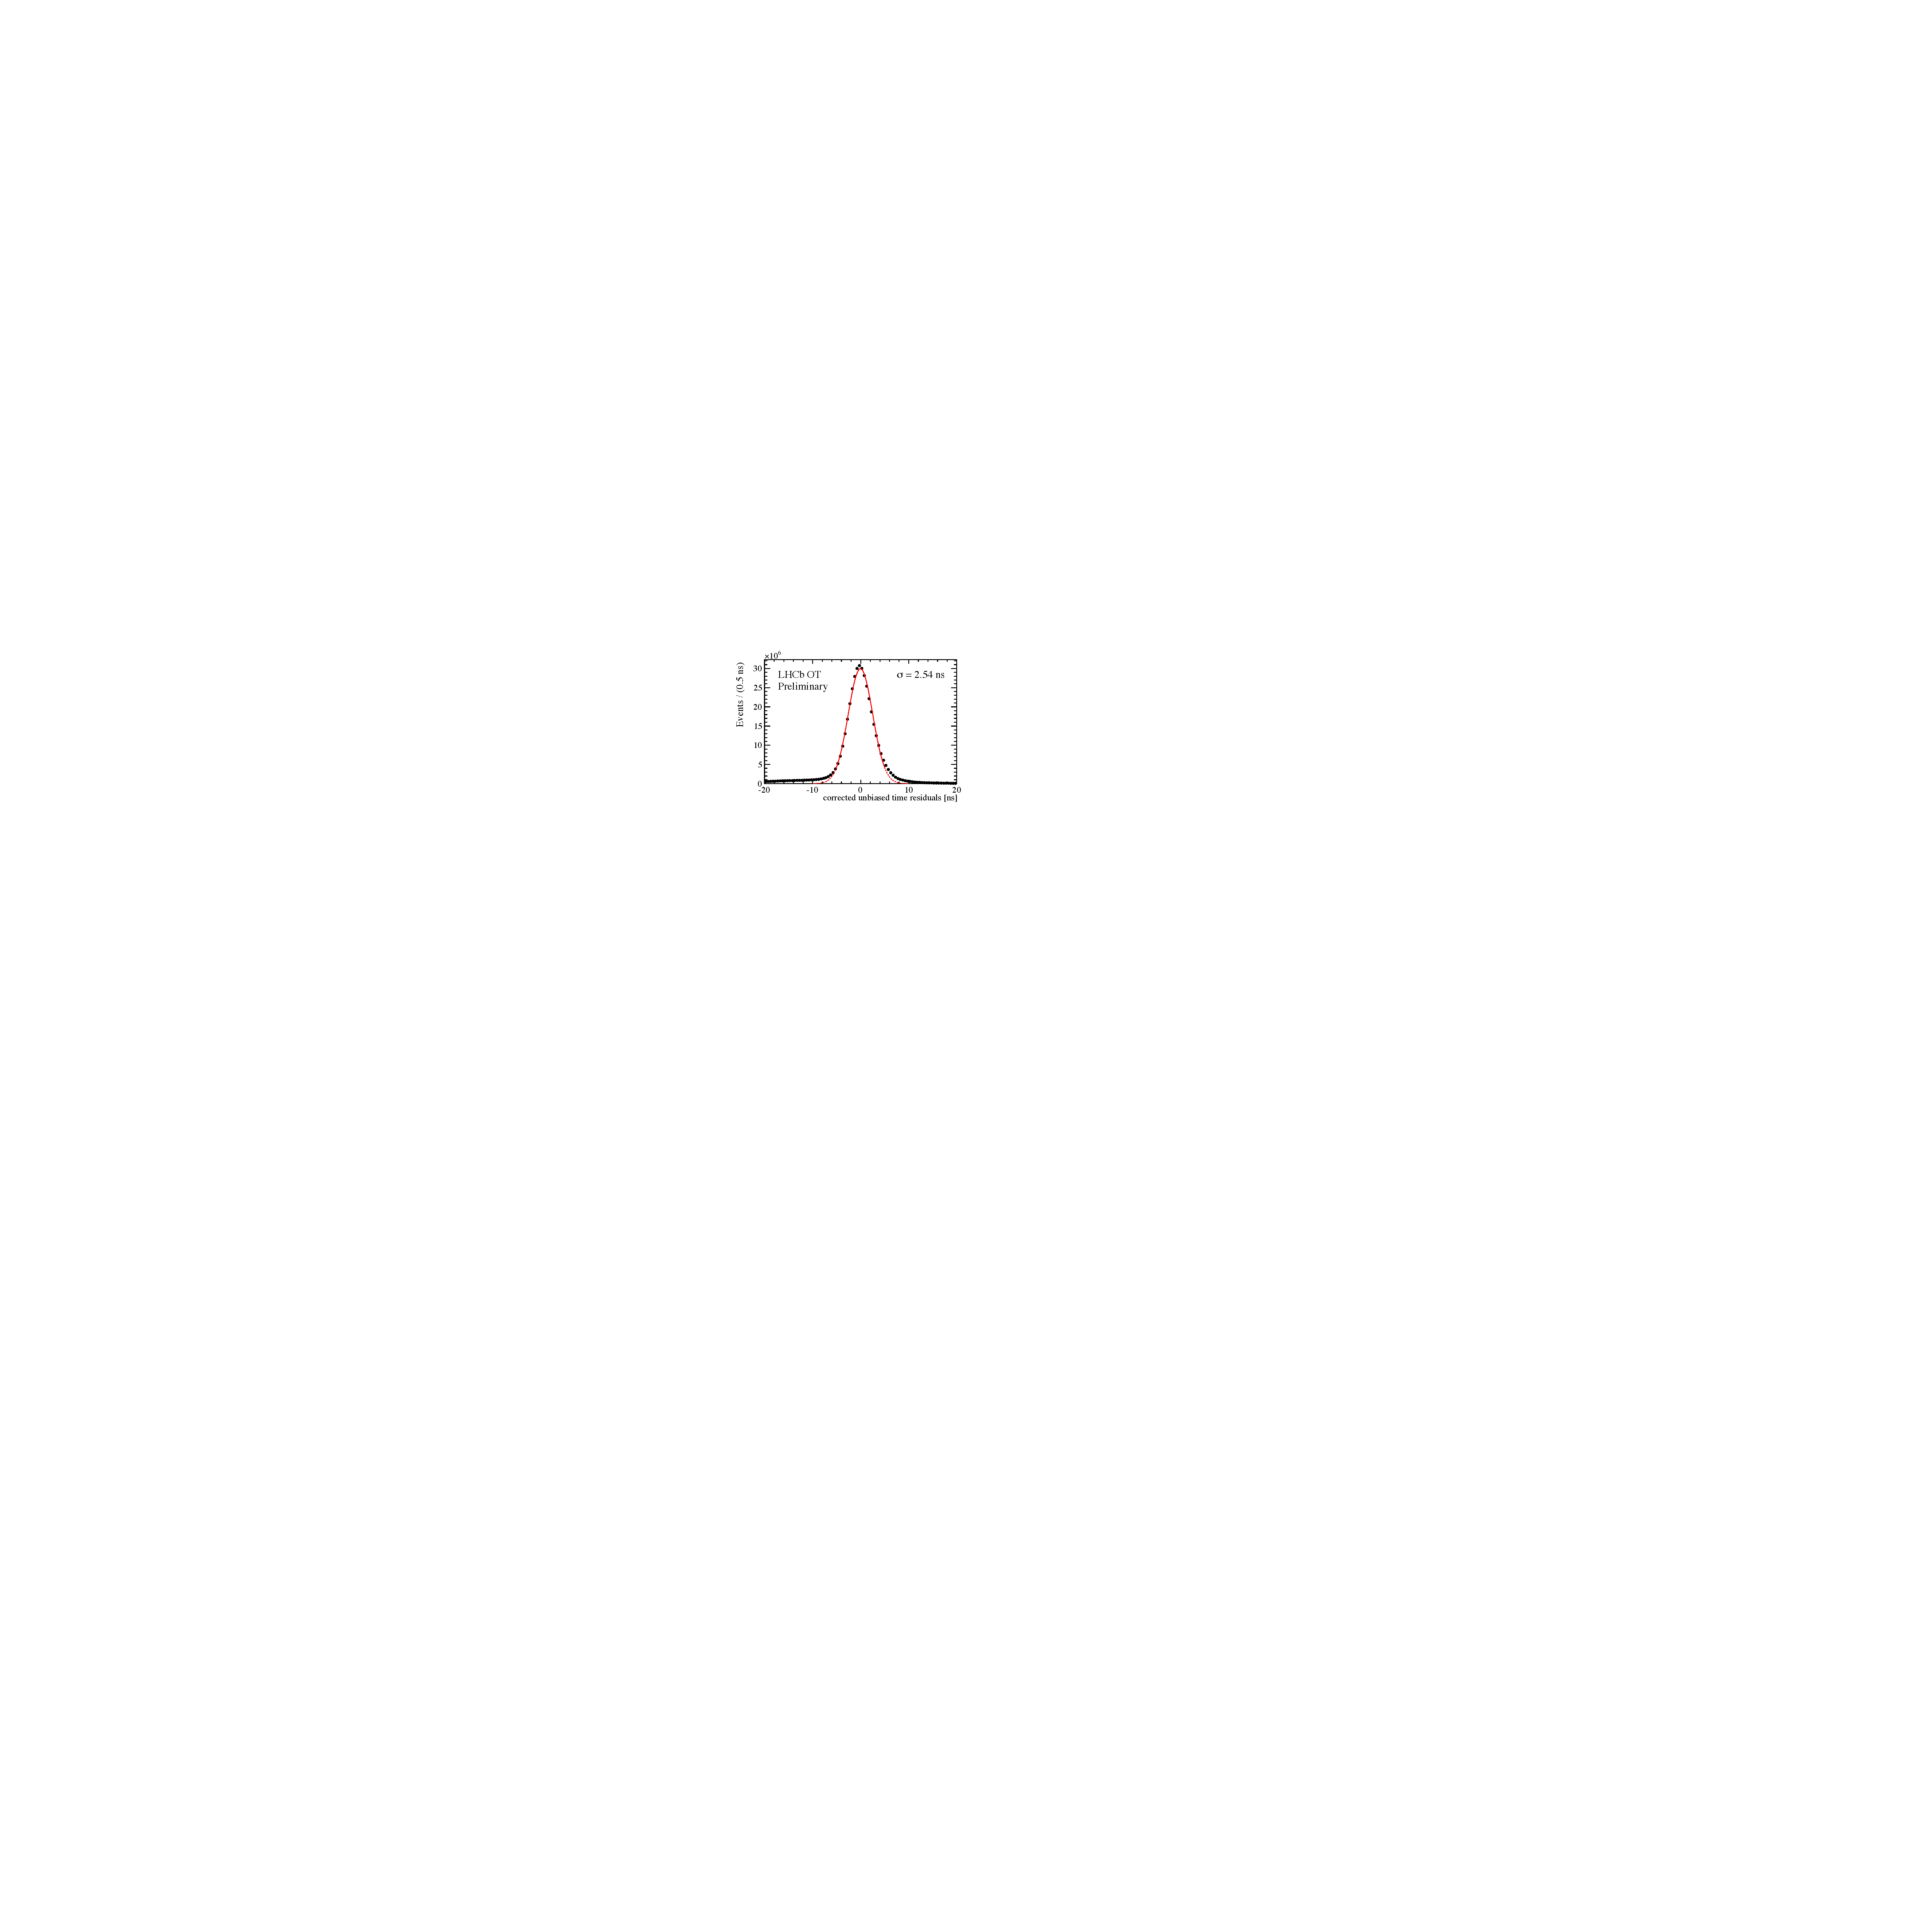
\includegraphics[width=0.6\textwidth]{figs/Detector/ot_resolution.pdf}
%     \caption{The \ttracker resolution, from Ref.~\cite{LHCb-DP-2014-002}.}
%     \label{fig:Dec_velo_leakage_current}   
% \end{figure}
% %%%%%%%%%%%%%%%%%%%%%%%%%%%%%%%%%%%%%%%%%%%%%%%%%%%%%%%%%%


\subsection{Ring imaging Cherenkov detectors}

The ring imaging Cherenkov detectors (\rich) provide essential information about the particle identification of tracks, allowing different hadronic species to be distinguished.
This allows kaons and protons to be distinguished from one another and the abundant pions tracks in a typical event. It can also help differentiate leptonic tracks in combination with the calorimeters and muon systems. 

Two \rich sub-detectors are present, each optimised for particles with different momentums. The first, \richone, is located between the \velo and \ttracker, before the particles have passed through the magnetic field. This provides discrimination primarily for low momentum tracks between 1--60\gevc. A second sub-detector, \richtwo, is located between the \intr and \ot tracking stations and calorimeters, after the particles have travelled through the magnetic field. This caters for the higher momentum particles in the range 15--100\gevc. 

The \rich detectors help to determine the species of the particles passing though it by capturing Cherenkov radiation emitted by the particle as it traverses a transparent medium referred to as a radiator. Cherenkov radiation is produced by particles travelling above the phase velocity of light in that specific medium. The radiation propagates at constant angle $\theta$ to the particles direction, determined by the speed of the particle $\beta = v/c$ and refractive index of the material $n$ as follows
\begin{equation}
\cos{\theta} = \frac{1}{\beta n}.
\end{equation}
This light is collected by mirrors and focussed onto light sensors. 

Although the particles produced in the collisions are all highly energetic and travelling close to the speed of light, the differences in the masses mean the species travel at slightly difference velocities. This then results in a different Cherenkov angle. In combination with the momentum measurement from the magnet spectrometer, different mass hypotheses can be compared. The Cherekov angles for different particle species as a function of momentum are shown in Fig.~\ref{fig:Dec_rich_species}. 


%%%%%%%%%%%%%%%%%%%%%%%%%%%%%%%%%%%%%%%%%%%%%%%%%%%%%%%%%%
\begin{figure}[!h]
    \centering
    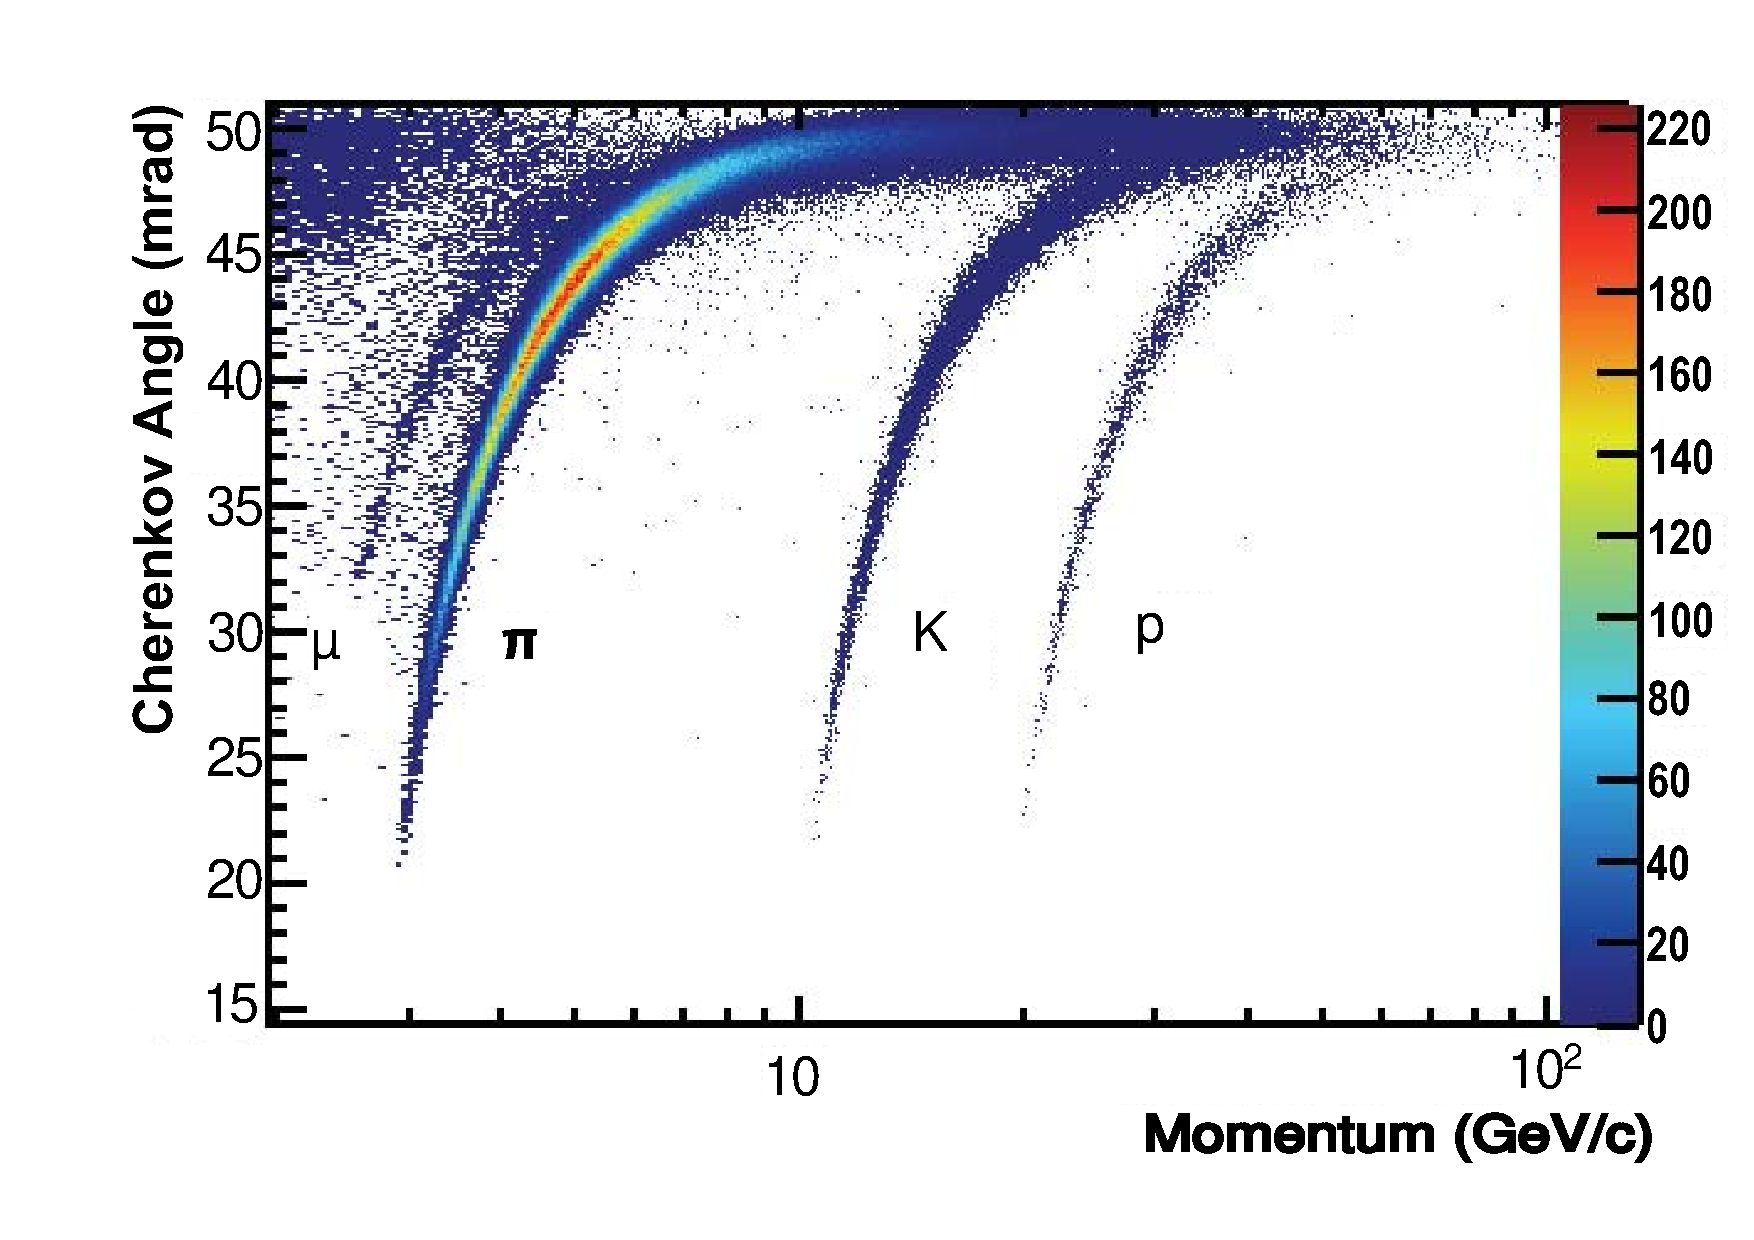
\includegraphics[width=0.6\textwidth]{figs/Detector/rich_speices.pdf}
    \caption{The Cherenkov angle for different species of particles as a function of momentum, from Ref.~\cite{LHCb-DP-2012-003}.}
    \label{fig:Dec_rich_species}   
\end{figure}
%%%%%%%%%%%%%%%%%%%%%%%%%%%%%%%%%%%%%%%%%%%%%%%%%%%%%%%%%%


In both \richone and \richtwo the cone of Cherenkov radiation is reflected of spherical and planar mirrors. This not only redirects the radiation onto Hybrid Photon Detectors (HPDs) situated outside of the acceptance but also focusses the radiation into a single ring.    
The radius of this ring is used to determine the Cherenkov angle $\theta$. 
The identity of particles is determined by comparing likelihood for a given ring of hits to have been created by various species. 
This is performed globally for all tracks in an event. All tracks are assumed to be pions as these are most abundant. The hypothesis of each is switched to $e$, $\mu$, $K$ and proton, leaving all other tracks unchanged, and the likelihood recomputed. The species resulting in the minimum value of the global event likelihood is kept. This is repeated until all tracks are set to their preferred hypothesis. 
The difference in the global event log-likelihood is then used to indicate the species of each track. Each species is determined relative to the pion hypothesis 
\begin{equation}
\text{DLL} = \Delta \log{\mathcal{L}(X-\pi)} = \log{\mathcal{L}(X)} - \log{\mathcal{L}(\pi)},
\end{equation}
where $\mathcal{L}(X)$ is the global event likelihood when the given track is of the species $X$.



% %%%%%%%%%%%%%%%%%%%%%%%%%%%%%%%%%%%%%%%%%%%%%%%%%%%%%%%%%%
% \begin{figure}[!h]
%     \centering
%     \begin{subfigure}[t]{0.4\textwidth}
%         \centering        
%         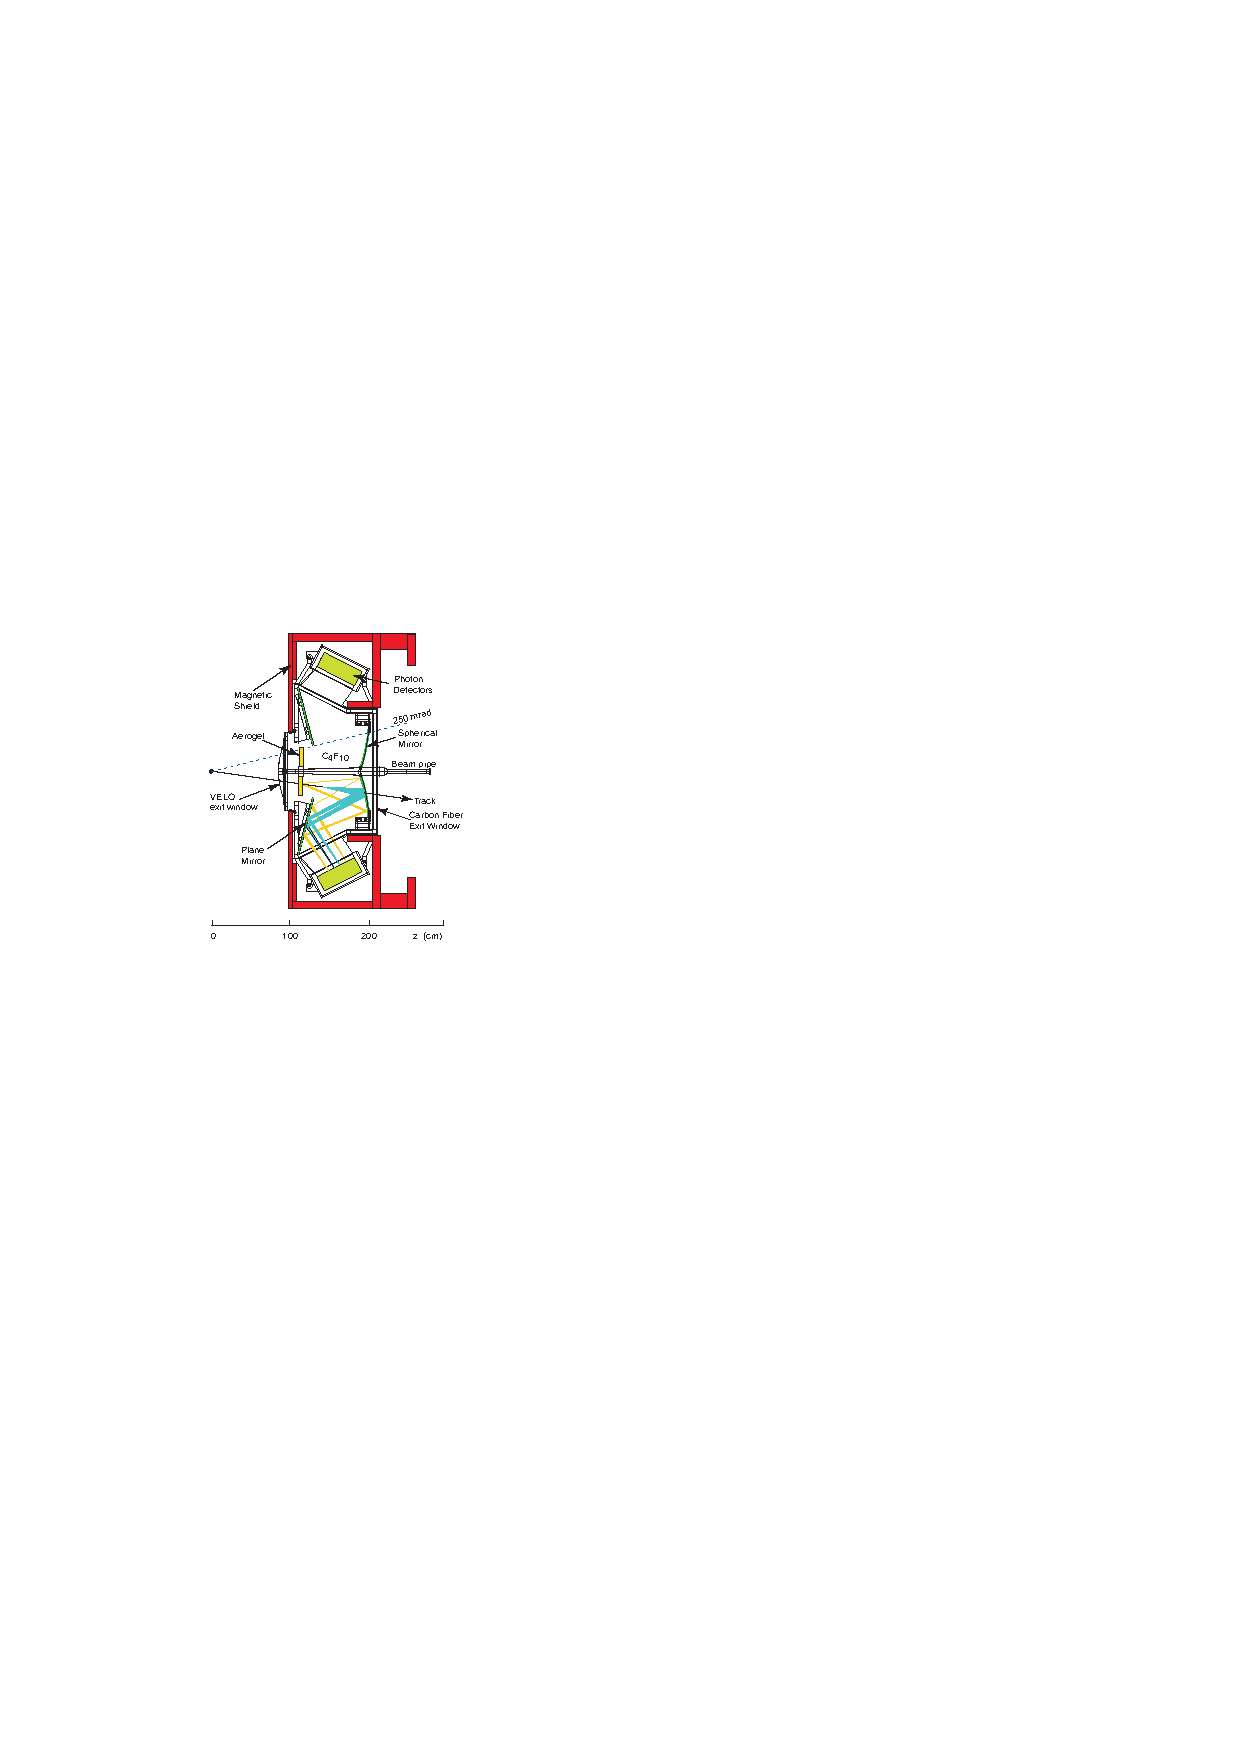
\includegraphics[width=1.0\textwidth]{figs/Detector/richone_layout.pdf}
%         \caption{\richone}
%     \end{subfigure}
%     \begin{subfigure}[t]{0.4\textwidth}
%         \centering
%         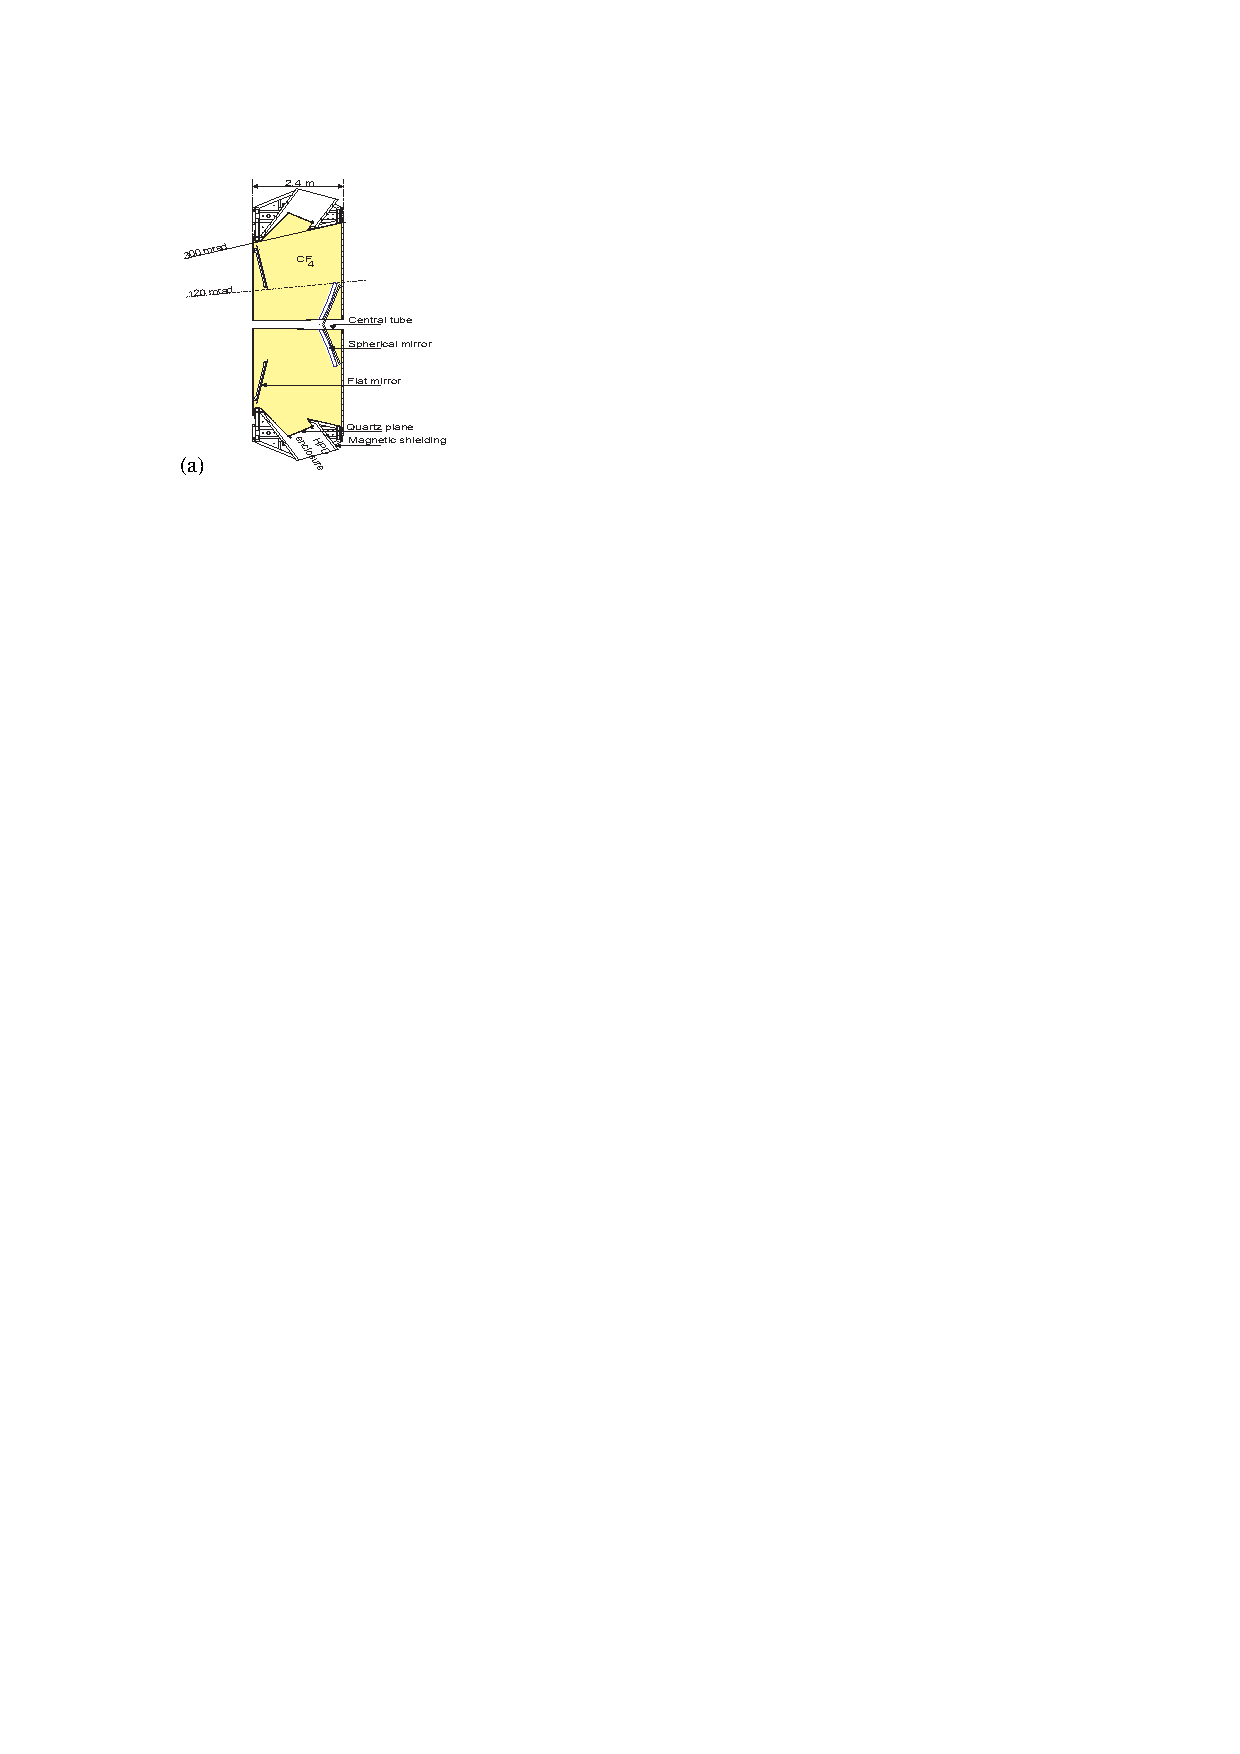
\includegraphics[width=1.0\textwidth]{figs/Detector/richtwo_layout.pdf}
%         \caption{\richtwo}
%     \end{subfigure}
%     \caption{Schematic the \richone and \richtwo sub-detectors, from Ref.~\cite{Alves:2008zz}.}

%     \label{fig:Dec_rich_layout}   
% \end{figure}
% %%%%%%%%%%%%%%%%%%%%%%%%%%%%%%%%%%%%%%%%%%%%%%%%%%%%%%%%%%




\subsubsection{\richone}
The \richone sub-detector was designed to aid particle identification for lower momentum tracks in the range 1--60\gevc using two radiators: aerogel and decafluorobutane ($\text{C}_{4}\text{F}_{10}$). These materials have refractive indices of $n = 1.030$ and $n = 1.0014$ respectively for $\lambda = 400\nm$ light. A diagram of the \richone detector as seen from the side is shown in Fig.~\ref{fig:Dec_richone_layout}. To minimise the amount of material that the particles pass through, the \richone detector is attached directly onto the \velo exit window.  

%%%%%%%%%%%%%%%%%%%%%%%%%%%%%%%%%%%%%%%%%%%%%%%%%%%%%%%%%%
\begin{figure}[!h]
    \centering        
    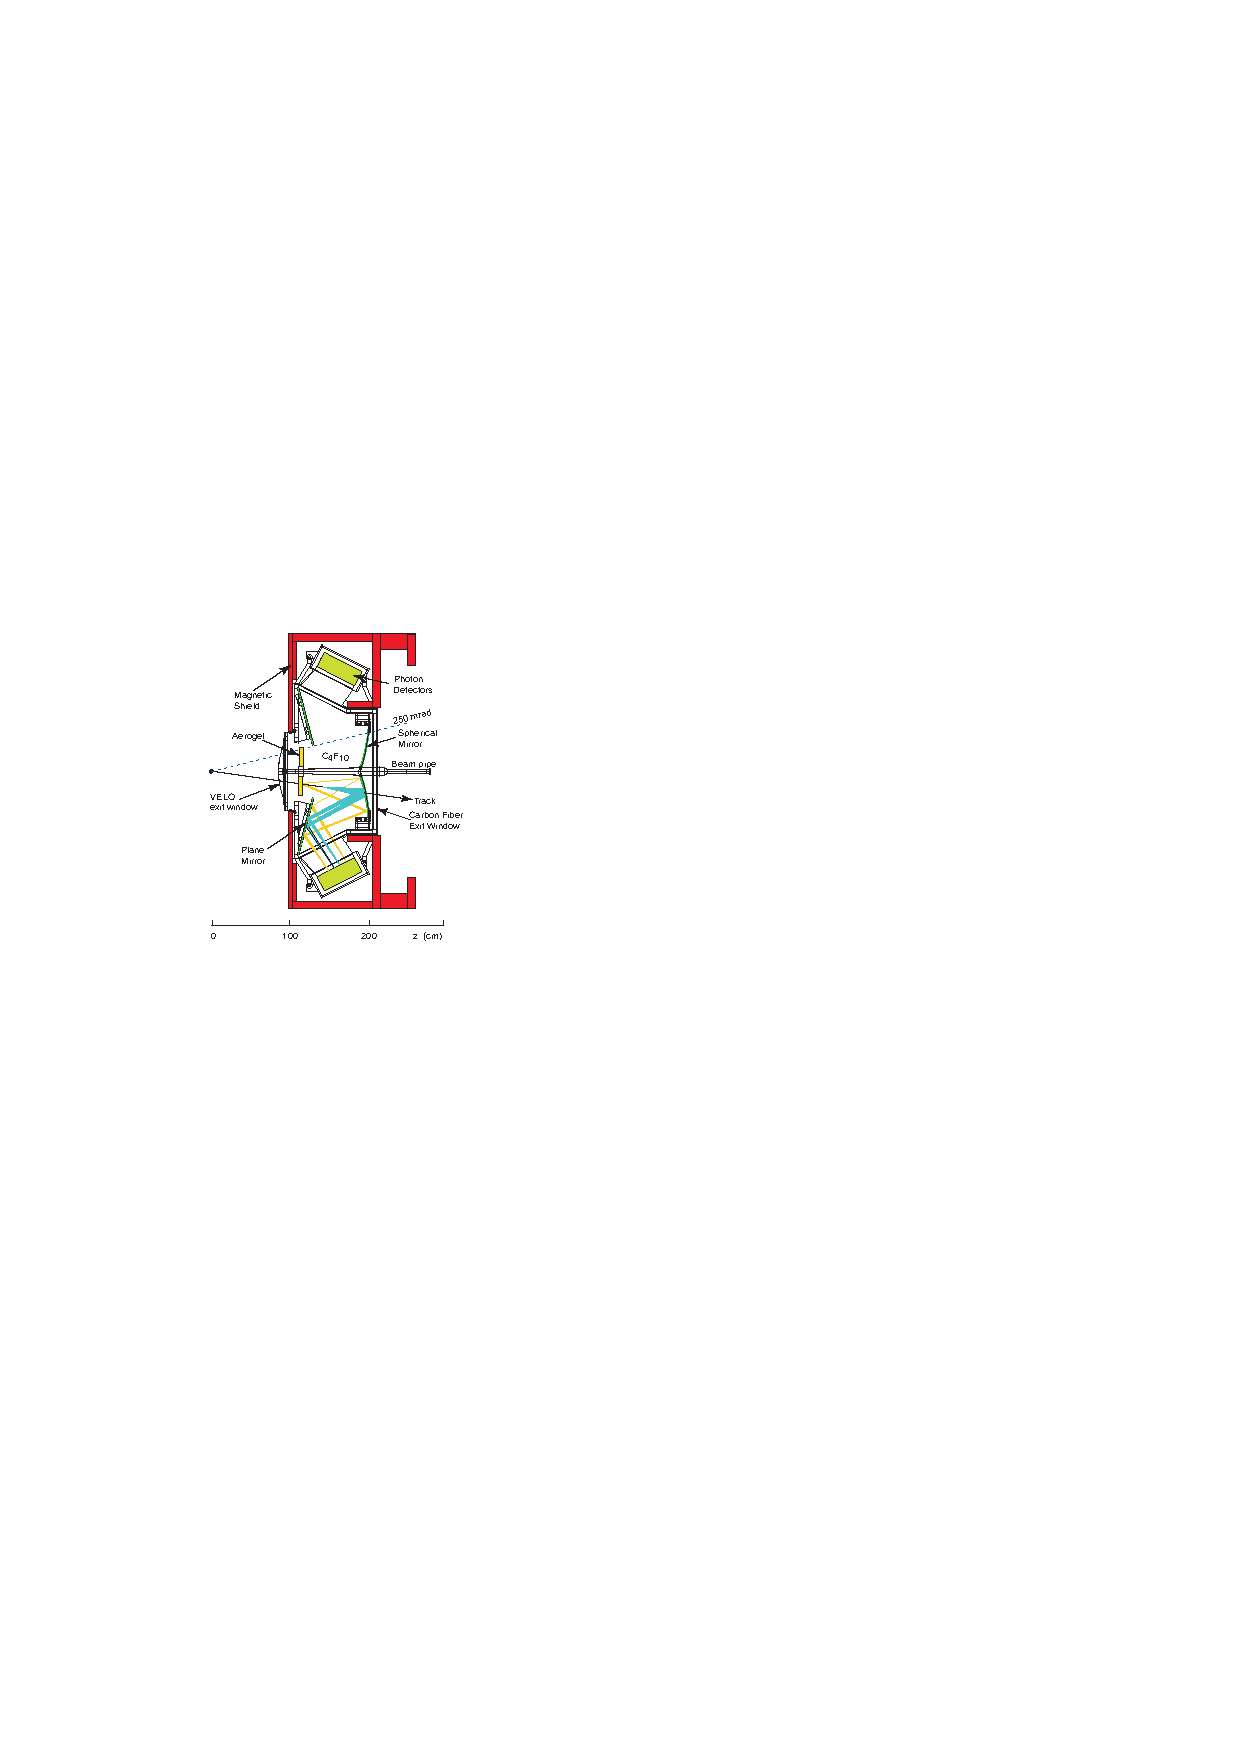
\includegraphics[width=0.4\textwidth]{figs/Detector/richone_layout.pdf}
    \caption{Schematic the \richone sub-detectors viewed from the side, from Ref.~\cite{Alves:2008zz}.}
    \label{fig:Dec_richone_layout}   
\end{figure}
%%%%%%%%%%%%%%%%%%%%%%%%%%%%%%%%%%%%%%%%%%%%%%%%%%%%%%%%%%

In Run II the aerogel was removed from the \richone detector. Although this catered specifically to the lower momentum tracks, the overall PID efficiency increased {\color{Red} Why?}. 


\subsubsection{\richtwo}

The \richtwo detector is designed to provide particle identification information for higher momentum tracks in the range 15--100\gevc using a single gas radiator tetrafluoromethane ($\text{C}\text{F}_{4}$). The refractive index for this material is $n=1.0005$ for $\lambda = 400\nm$ light.

%%%%%%%%%%%%%%%%%%%%%%%%%%%%%%%%%%%%%%%%%%%%%%%%%%%%%%%%%%
\begin{figure}[!h]
    \centering        
    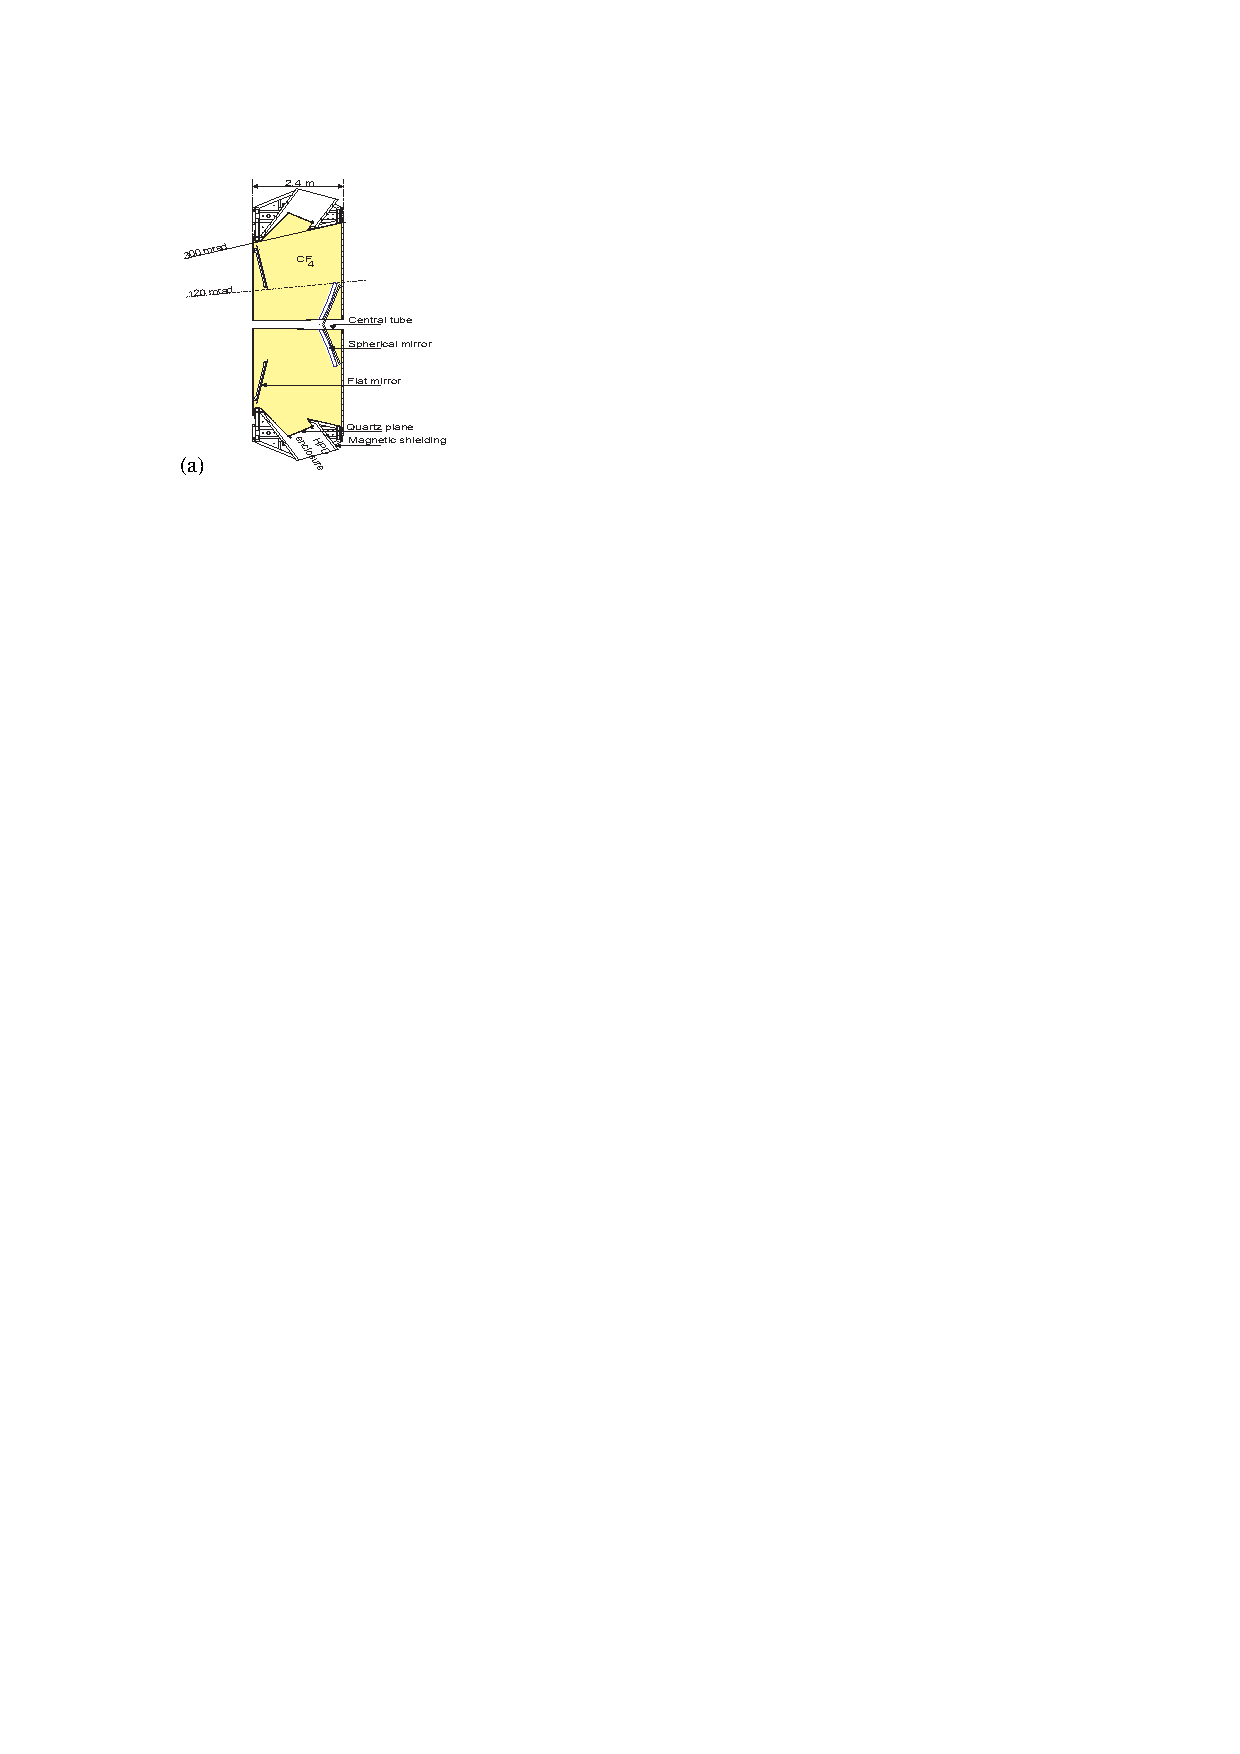
\includegraphics[width=0.4\textwidth]{figs/Detector/richtwo_layout.pdf}
    \caption{Schematic the \richtwo sub-detector viewed from above, from Ref.~\cite{Alves:2008zz}.}
    \label{fig:Dec_richtwo_layout}   
\end{figure}
%%%%%%%%%%%%%%%%%%%%%%%%%%%%%%%%%%%%%%%%%%%%%%%%%%%%%%%%%%



\subsubsection{Performance}
The performance of the \rich detectors can be quantified in terms of the selection efficiency and misidentification rates for different pairs of species. The efficiency of kaon identification and rate of pions being misidentified as kaons is shown in Fig.~\ref{fig:Dec_rich_k_pi} for Run I and Run II.  

%%%%%%%%%%%%%%%%%%%%%%%%%%%%%%%%%%%%%%%%%%%%%%%%%%%%%%%%%%
\begin{figure}[!h]
    \centering
    \begin{subfigure}[t]{0.4\textwidth}
        \centering        
        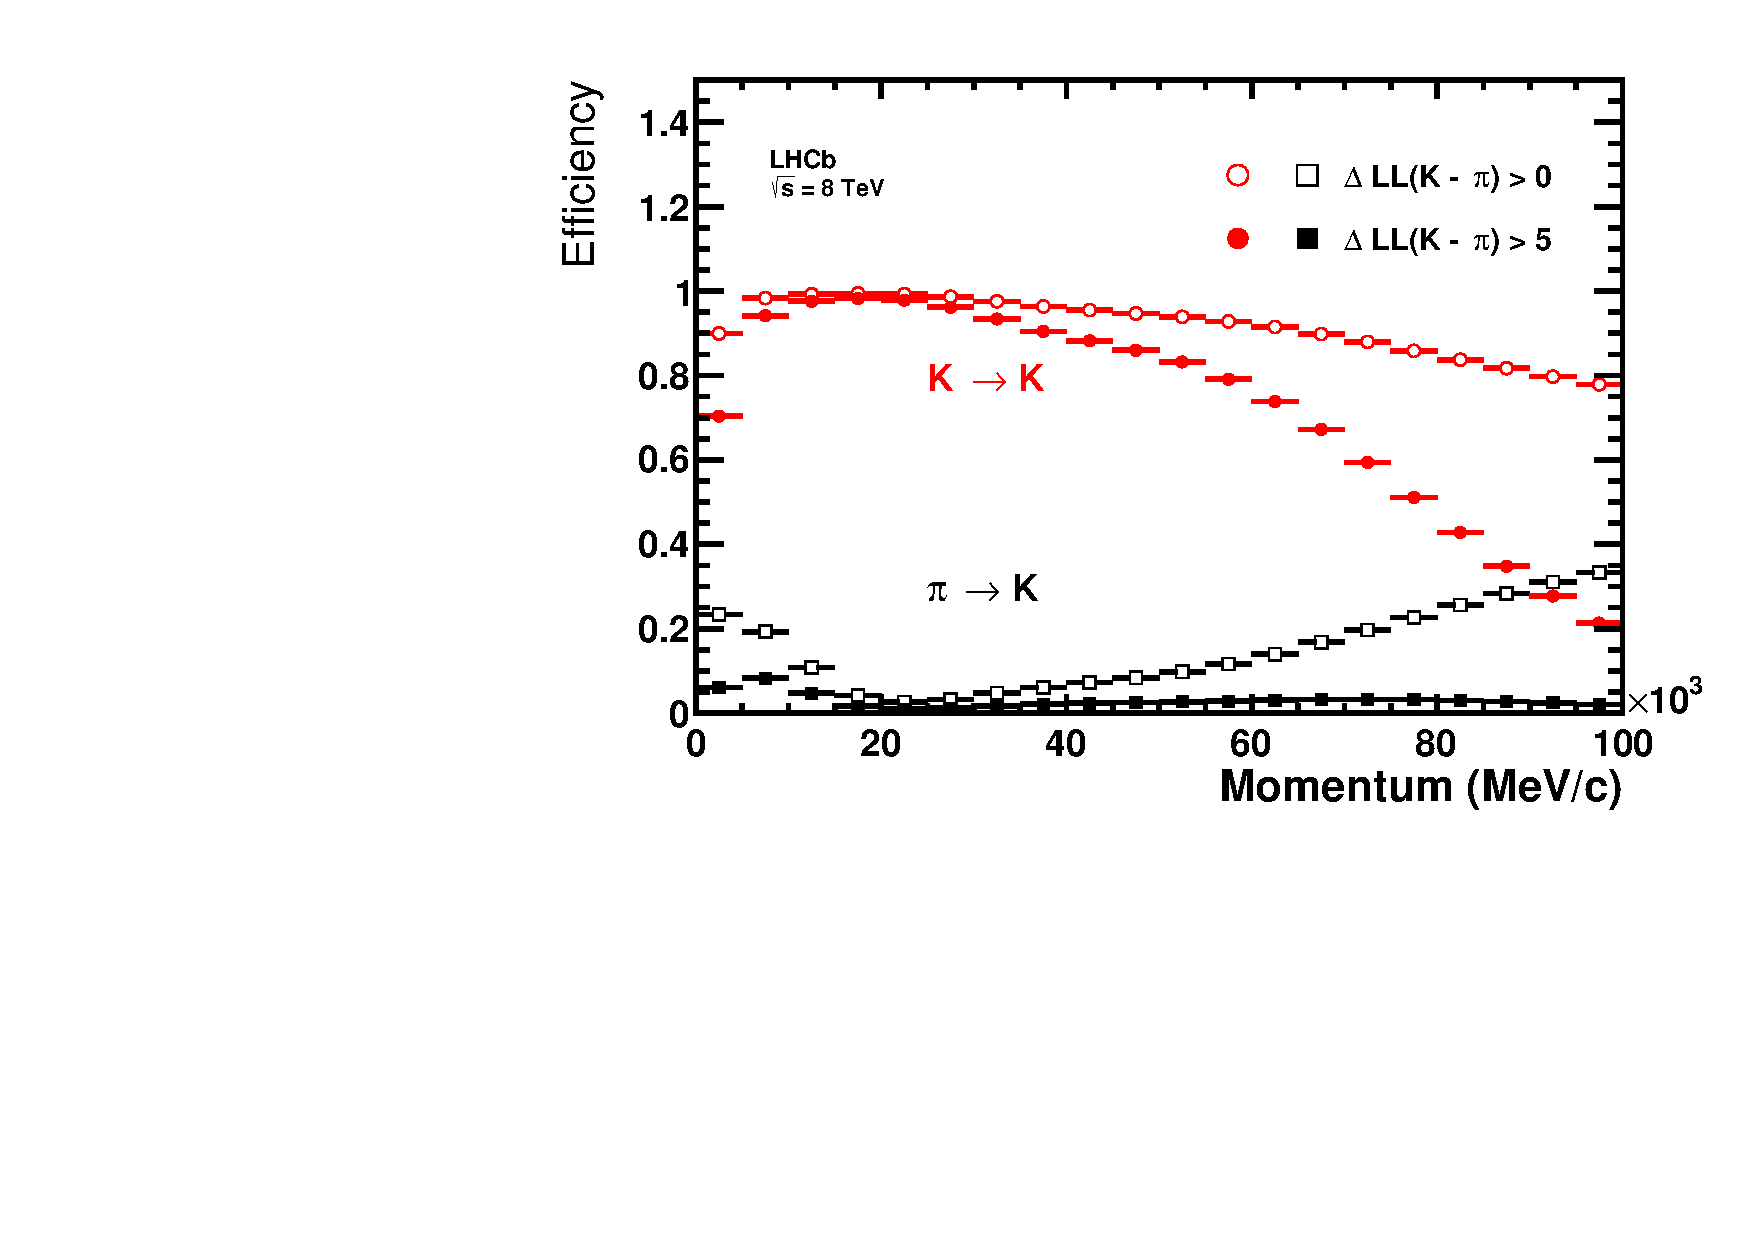
\includegraphics[width=1.0\textwidth]{figs/Detector/rich_k_pi_2012.pdf}
        \caption{2012}
    \end{subfigure}
    \begin{subfigure}[t]{0.4\textwidth}
        \centering
        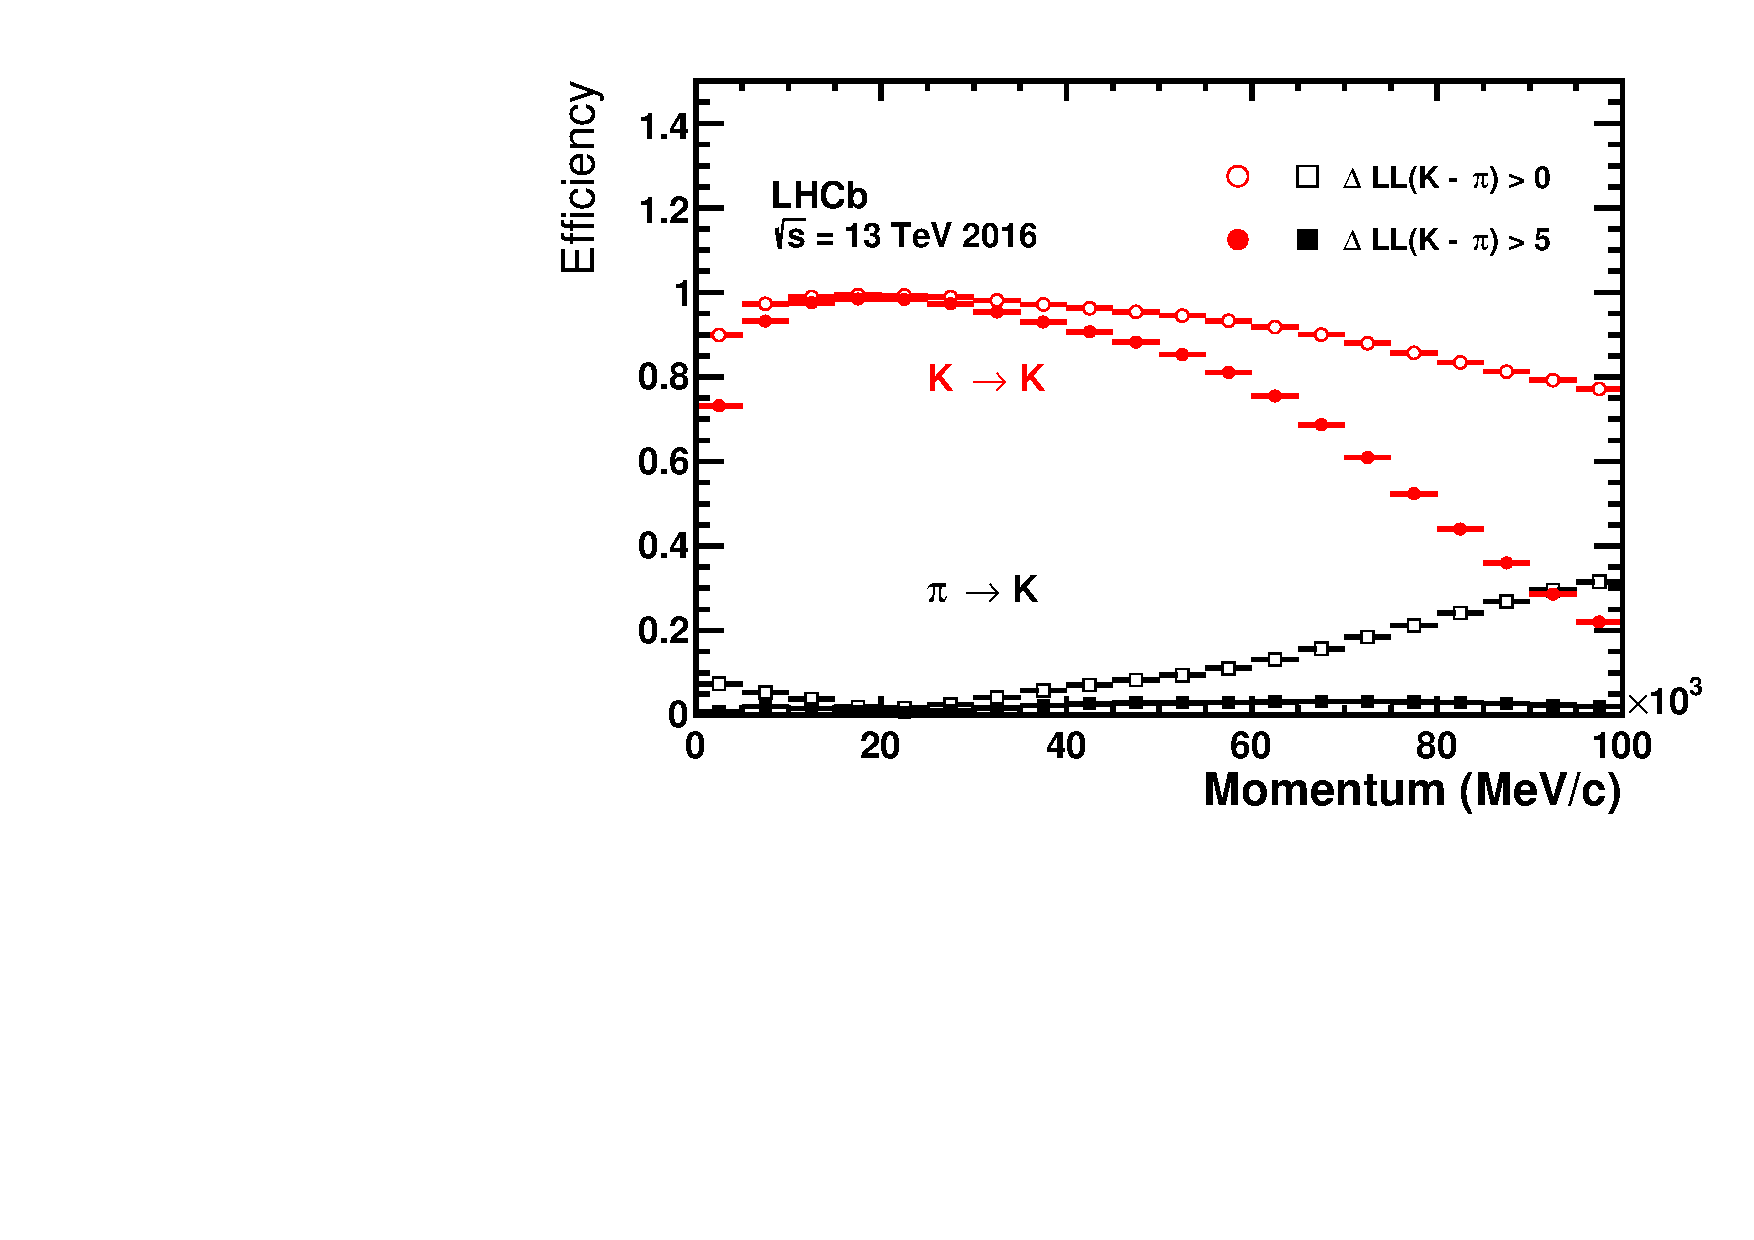
\includegraphics[width=1.0\textwidth]{figs/Detector/rich_k_pi_2016.pdf}
        \caption{2016}
    \end{subfigure}
    \caption{The \rich detector performance for kaon and pion separation, from Ref.~\cite{LHCb-DP-2012-003}.}
    \label{fig:Dec_rich_k_pi}   
\end{figure}
%%%%%%%%%%%%%%%%%%%%%%%%%%%%%%%%%%%%%%%%%%%%%%%%%%%%%%%%%%


\subsection{Calorimeters}

The calorimetry system is made of four components that work together to serve a number of purposes. 
Primarily, the detectors measure energy deposited by particles, vital for neutral pions or photons that don't interact with the tracking stations. Additionally, the calorimeters provide fast measurements of the energy deposited by interacting particles, suitable for use in the trigger. Finally, the four components work together to improve the discrimination of different particle species, in particular between electrons and hadrons. 



All of the calorimeter components work on the same basic principle; the particles pass through a transparent materials producing a flash of light, known as scintillation light. This light is collected and measured; the quantity determines the energy deposited by the particle.  



%%%%%%%%%%%%%%%%%%%%%%%%%%%%%%%%%%%%%%%%%%%%%%%%%%%%%%%%%%
\begin{figure}[!h]
    \centering
    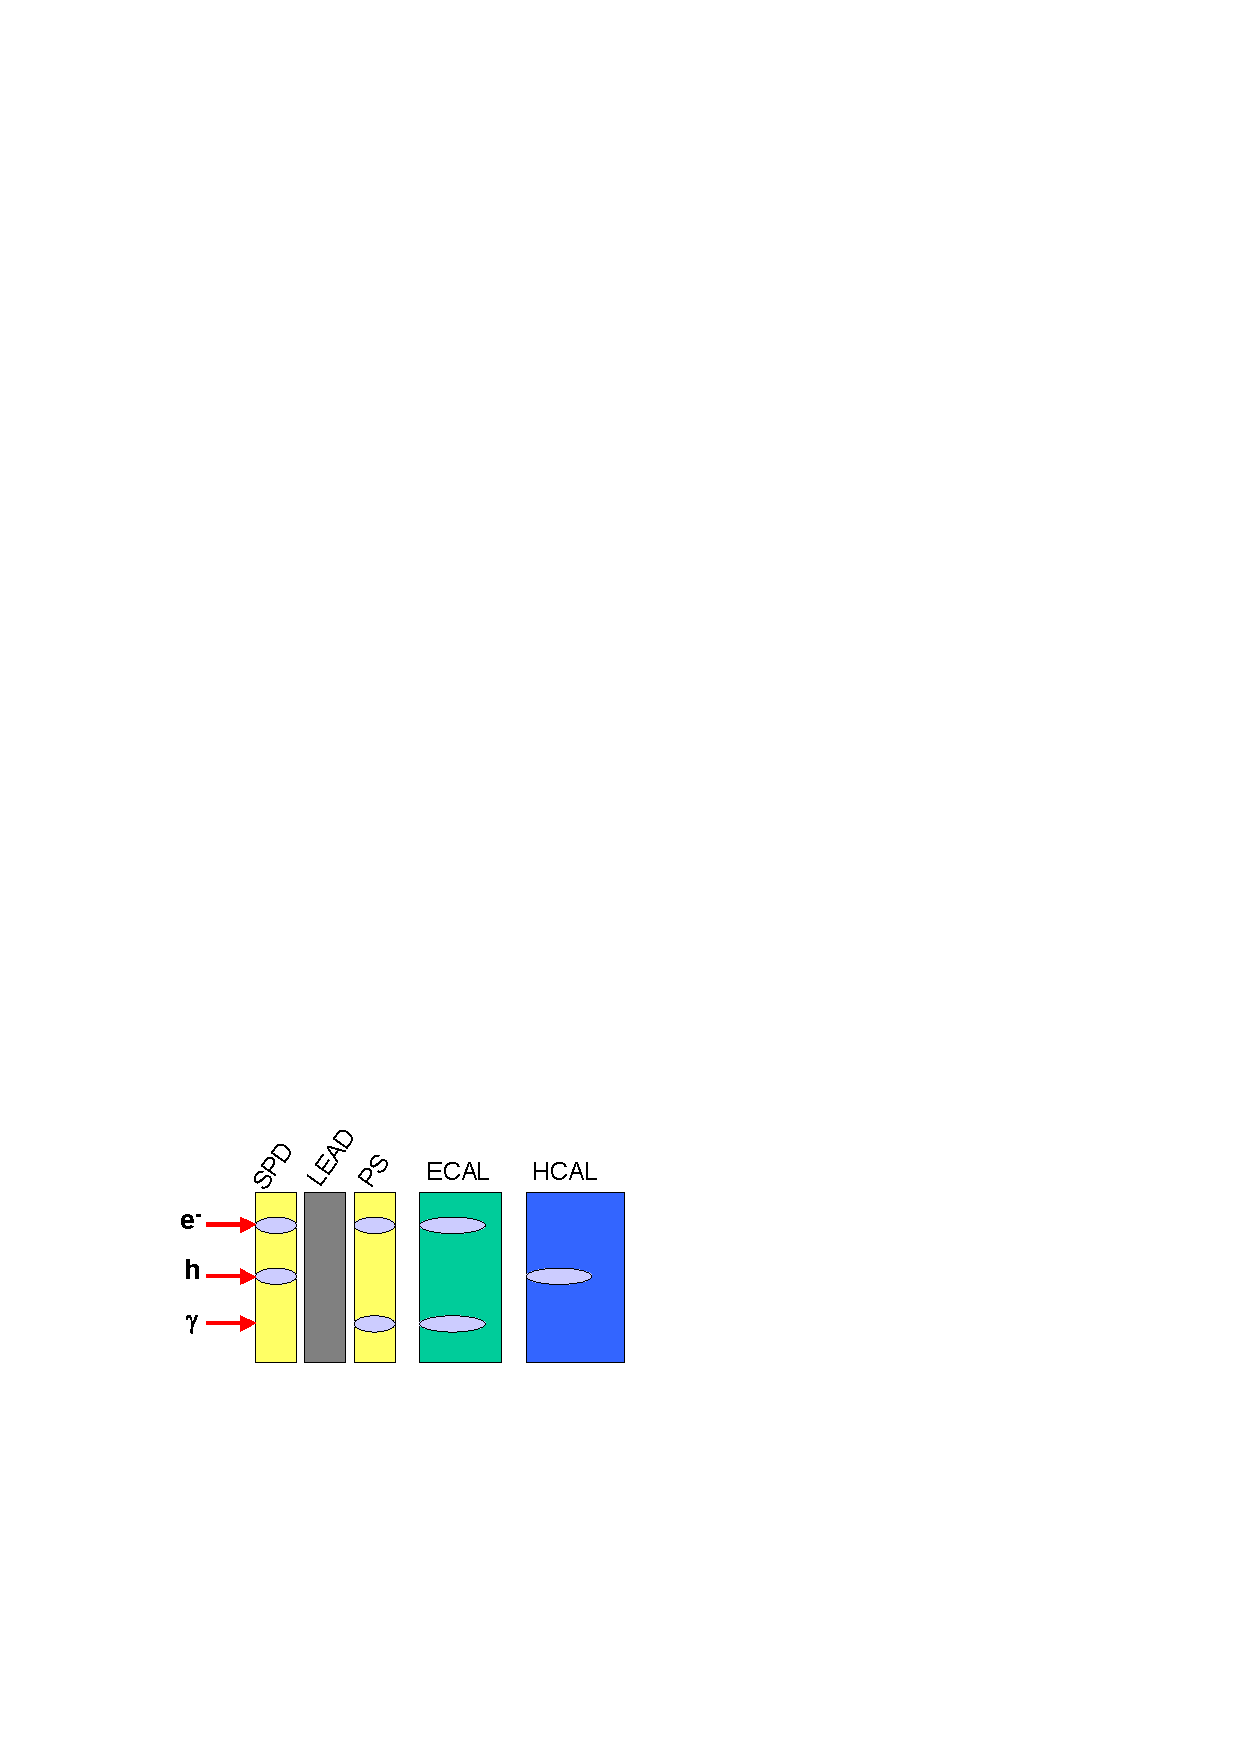
\includegraphics[width=0.6\textwidth]{figs/Detector/calo_layout.pdf}
    \caption{A diagram illustrating how the calorimeter system aids particle identification, from Ref.~\cite{1742-6596-293-1-012059}.}
    \label{fig:Dec_calo_layout}   
\end{figure}
%%%%%%%%%%%%%%%%%%%%%%%%%%%%%%%%%%%%%%%%%%%%%%%%%%%%%%%%%%


The first layer of the calorimeter system is the scintillator pad detector (\spd), as shown in Fig.~\ref{fig:Dec_calo_layout}. This provides information about whether the incident particles are neutral or charged. After this comes the pre-shower detector (\presh). This indicates the electromagnetic nature of the of the particle. For charged particles this separates electrons and charged hadrons; for neutral particle it helps separate photons from neutral hadrons. Next comes the electromagnetic calorimeter (\ecal) tasked with measuring the energy of electromagnetically interacting particles, including electrons and photons. Finally, the hadronic calorimeter (\hcal) determines the energy deposited by hadrons, including pions, kaons, protons and neutrons. 

\subsubsection{Scintillator pad detector and Pre-shower detector}

The \spd and \presh are almost identical scintillating pads detectors constructed from a mix of polystyrene and wavelength-shifting dopants. The pads are coated in light-proof paper and contain loops of wavelength-shifting fibres to collect the scintillation light. The pads are segmented into cells, matching the granularity of the \ecal detector.
The fibres are connected to long clear fibres connected to photo-multiplier tubes (PMT) outside the detectors acceptance. Between the \spd and \presh detectors is a 15\mm thick layer of lead. This layer initiates electrons and photons to interact electromagnetically, depositing some of their energy in the \presh scintillating pads.    


\subsubsection{Electronic Calorimeter}


The \ecal is made of 66 layers of alternating lead and scintillator, with a total depth of 42\cm. This thickness corresponds to 25 radiation lengths. The layout of the layers are shown in Fig.~\ref{fig:Dec_ecal_layout}. Scintillating light is captured and transported by wavelength-shifting wires that pass through the entire structure. The light is measured by PMTs positioned at the end of the structure. The cells of the \ecal are segmented differently depending on the proximity to the beam-pipe, as shown in Fig.~\ref{fig:Dec_ecal_layout}. The cells are split into inner, middle and outer regions with sizes $4\times 4\cm$, $6\times 6\cm$ and $12\times 12\cm$ respectively. 

%%%%%%%%%%%%%%%%%%%%%%%%%%%%%%%%%%%%%%%%%%%%%%%%%%%%%%%%%%
\begin{figure}[!h]
    \centering
    \begin{subfigure}[m]{0.4\textwidth}
        \centering        
        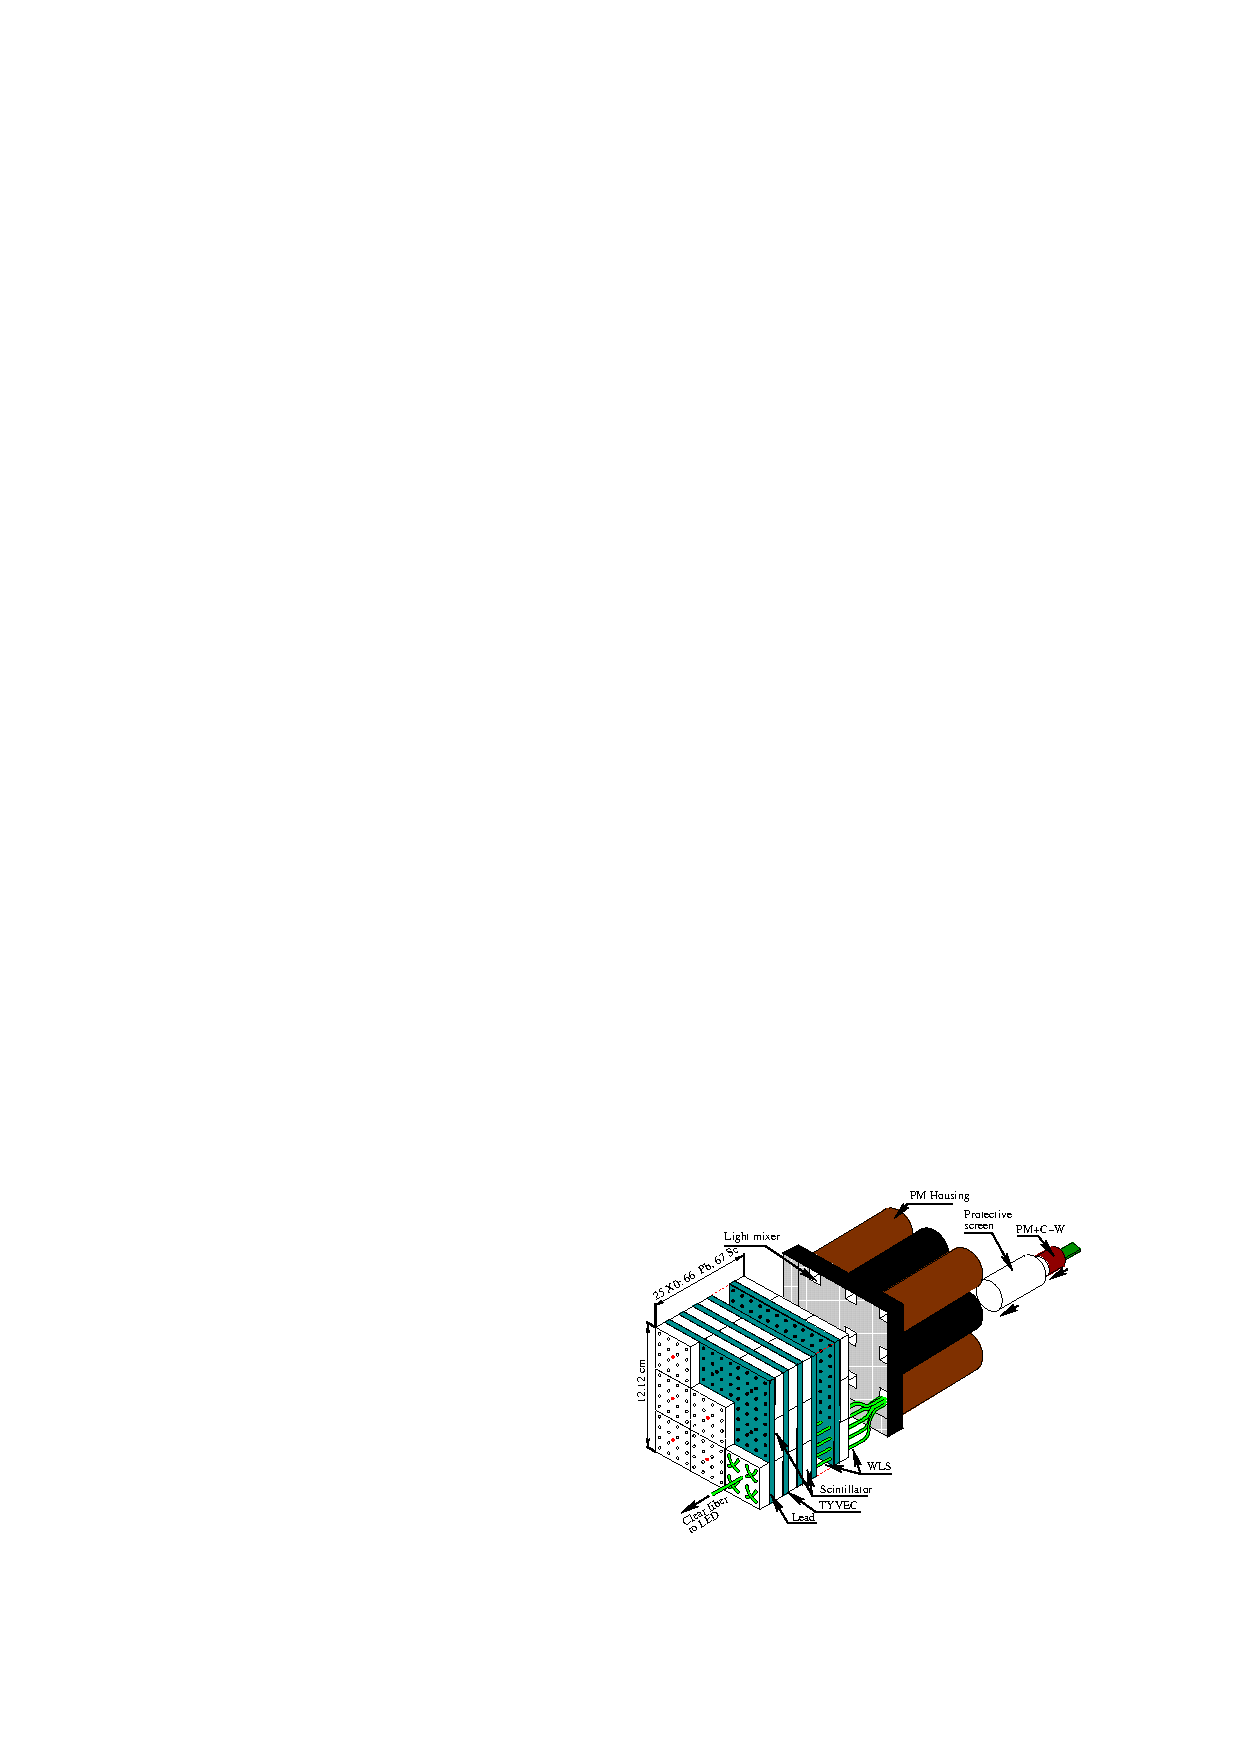
\includegraphics[width=1.0\textwidth]{figs/Detector/ecal_diagram.pdf}
    \end{subfigure}
    \begin{subfigure}[m]{0.4\textwidth}
        \centering
        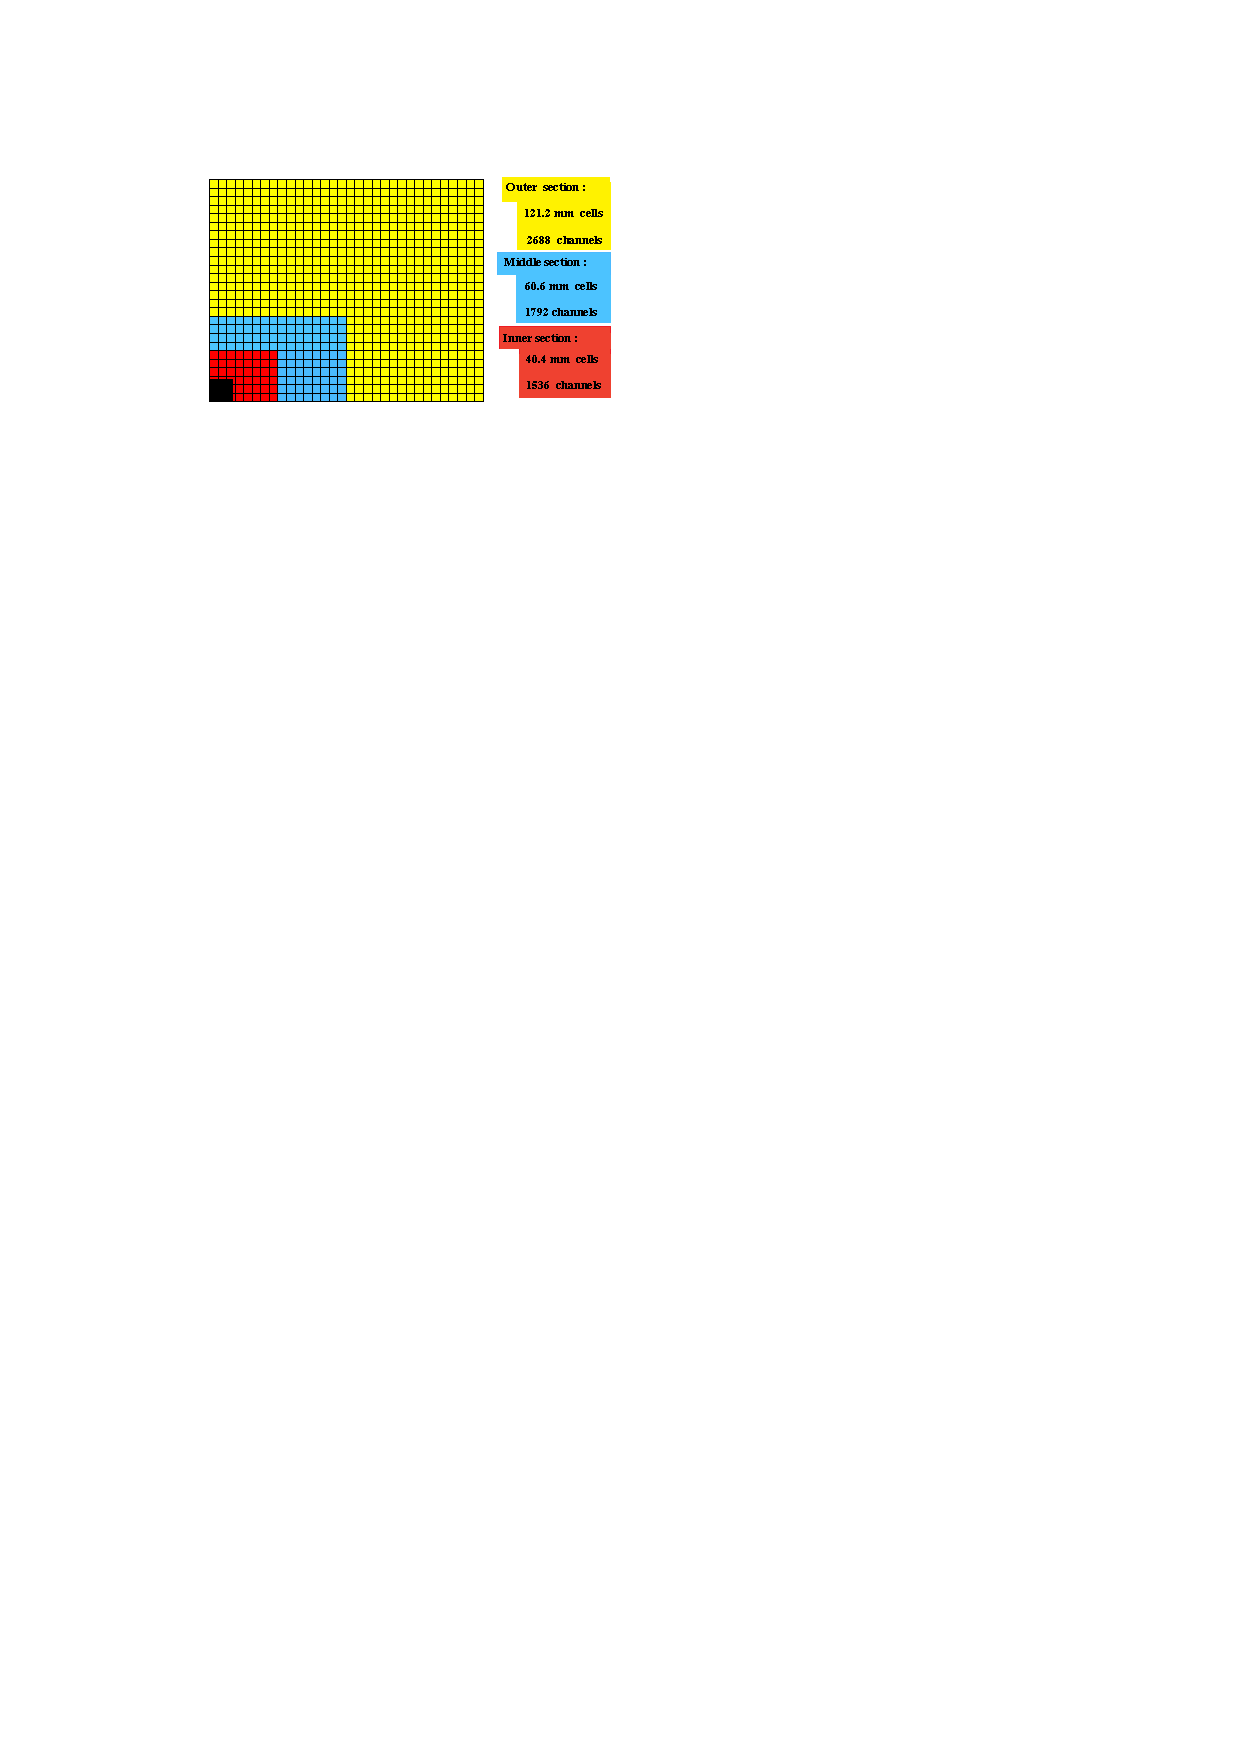
\includegraphics[width=1.0\textwidth]{figs/Detector/ecal_layout.pdf}
    \end{subfigure}
    \caption{A diagram of one of the inner \ecal modules (left) and the layout of one quarter of the \ecal modules (right), from Ref.~\cite{Alves:2008zz} and Ref.~\cite{doi:1765047}.}
    \label{fig:Dec_ecal_layout}   
\end{figure}
%%%%%%%%%%%%%%%%%%%%%%%%%%%%%%%%%%%%%%%%%%%%%%%%%%%%%%%%%%

{\color{Red}
\begin{itemize}
\item Find resolution
\end{itemize}
}

\subsubsection{Hadronic calorimeter}

The \hcal is a 500 tonne detector constructed from iron plates and scintillating tiles. Unlike the \ecal, these are arranged parallel to the beam-pipe as shown in Fig.~\ref{fig:Dec_hcal_layout}. The cells vary in size in the different regions of the detector; the inner regions correspond to $13 \times 13 \cm$ cells and the outer to $26\times26\cm$. The widths of the iron tiles are chosen to be one radiation length (1\cm), and the lengths are one hadron interaction length. The scintillation light is collected by wavelength-shifting fibres that are read out by PMTs located at the rear of each cell.    

{\color{Red}
\begin{itemize}
\item Find resolution
\end{itemize}
}

%%%%%%%%%%%%%%%%%%%%%%%%%%%%%%%%%%%%%%%%%%%%%%%%%%%%%%%%%%
\begin{figure}[!h]
    \centering
    \begin{subfigure}[m]{0.4\textwidth}
        \centering        
        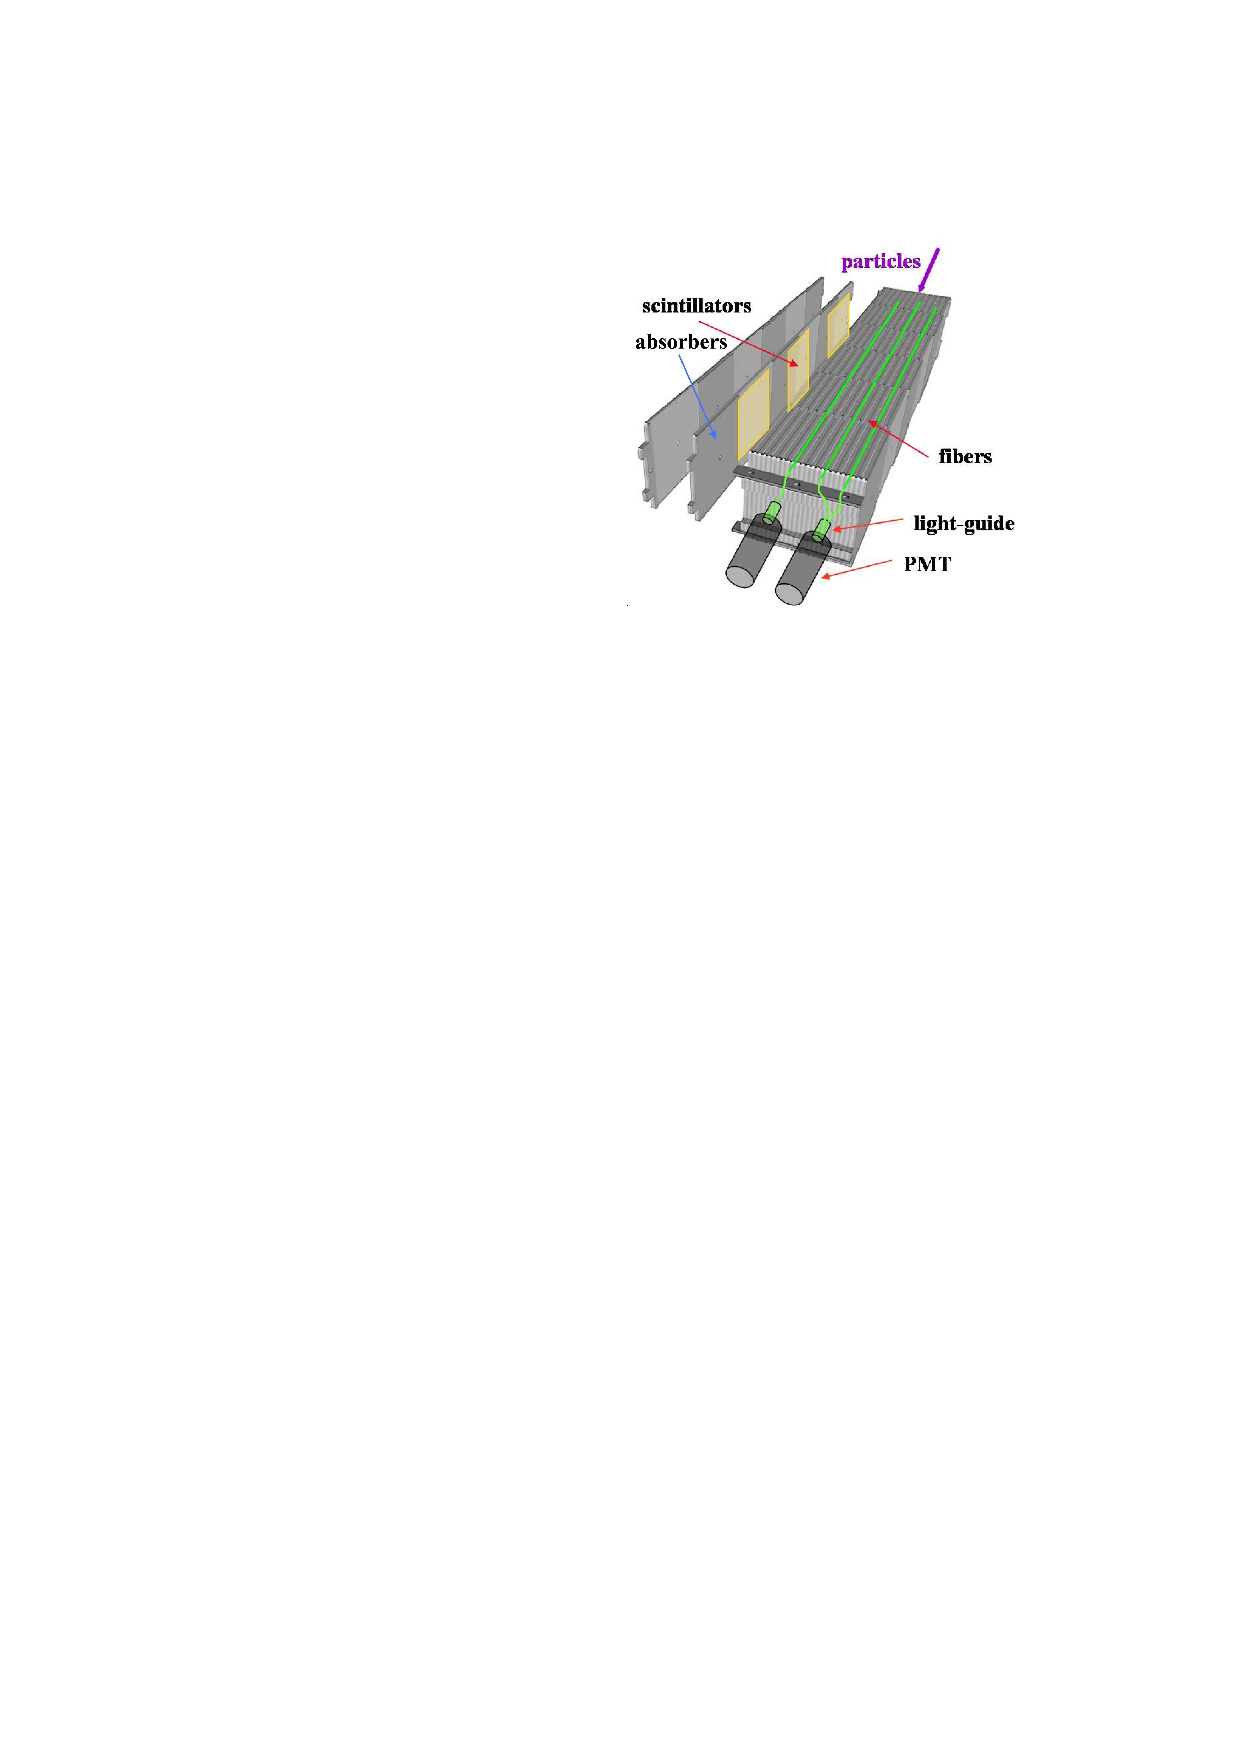
\includegraphics[width=1.0\textwidth]{figs/Detector/hcal_diagram.pdf}
    \end{subfigure}
    \begin{subfigure}[m]{0.4\textwidth}
        \centering
        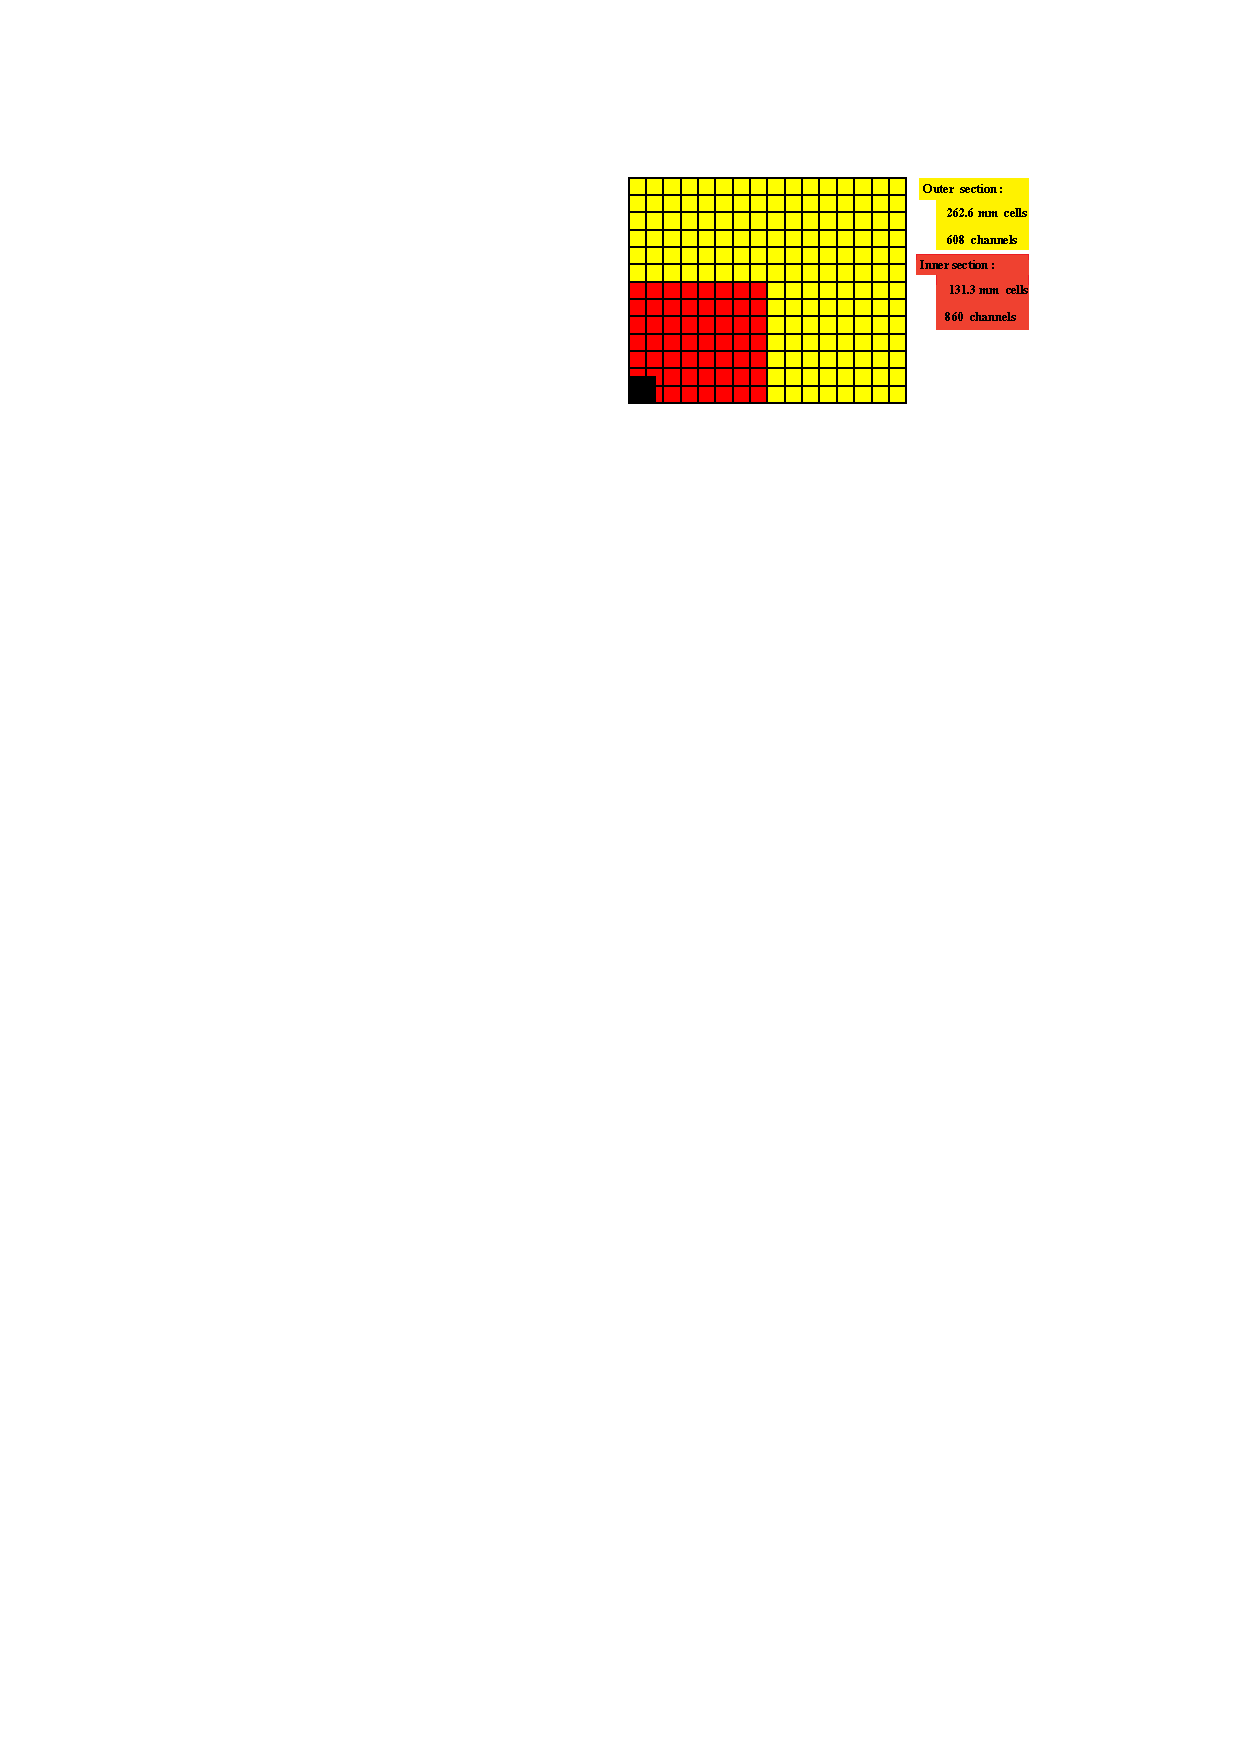
\includegraphics[width=1.0\textwidth]{figs/Detector/hcal_layout.pdf}
    \end{subfigure}
    \caption{A diagram of one of the \hcal modules (left) and the layout of one quarter of the \hcal modules (right), from Ref.~\cite{Alves:2008zz}.}
    \label{fig:Dec_hcal_layout}   
\end{figure}
%%%%%%%%%%%%%%%%%%%%%%%%%%%%%%%%%%%%%%%%%%%%%%%%%%%%%%%%%%

\subsection{Muon system}


The muon system serves two main purposes: to provide fast muon \pt measurements for use in the hardware trigger; and to provide muon identification information for use in the software trigger and offline analyses.
The muon system is made of five rectangular stations. The first (M1) is positioned before the calorimeters and the remaining (M2--M4) are positioned after, as shown in Fig.~\ref{fig:Dec_muon_schematic}. The latter stations alternate with 80\cm layers of iron absorbers. The muon system is the last sub-detector as muons are highly penetrating particles, travelling through more material than other species. The interleaving iron absorbers help to isolate muons, as other particles are stopped by these layers. 

% %%%%%%%%%%%%%%%%%%%%%%%%%%%%%%%%%%%%%%%%%%%%%%%%%%%%%%%%%%
% \begin{figure}[!h]
%     \centering
%     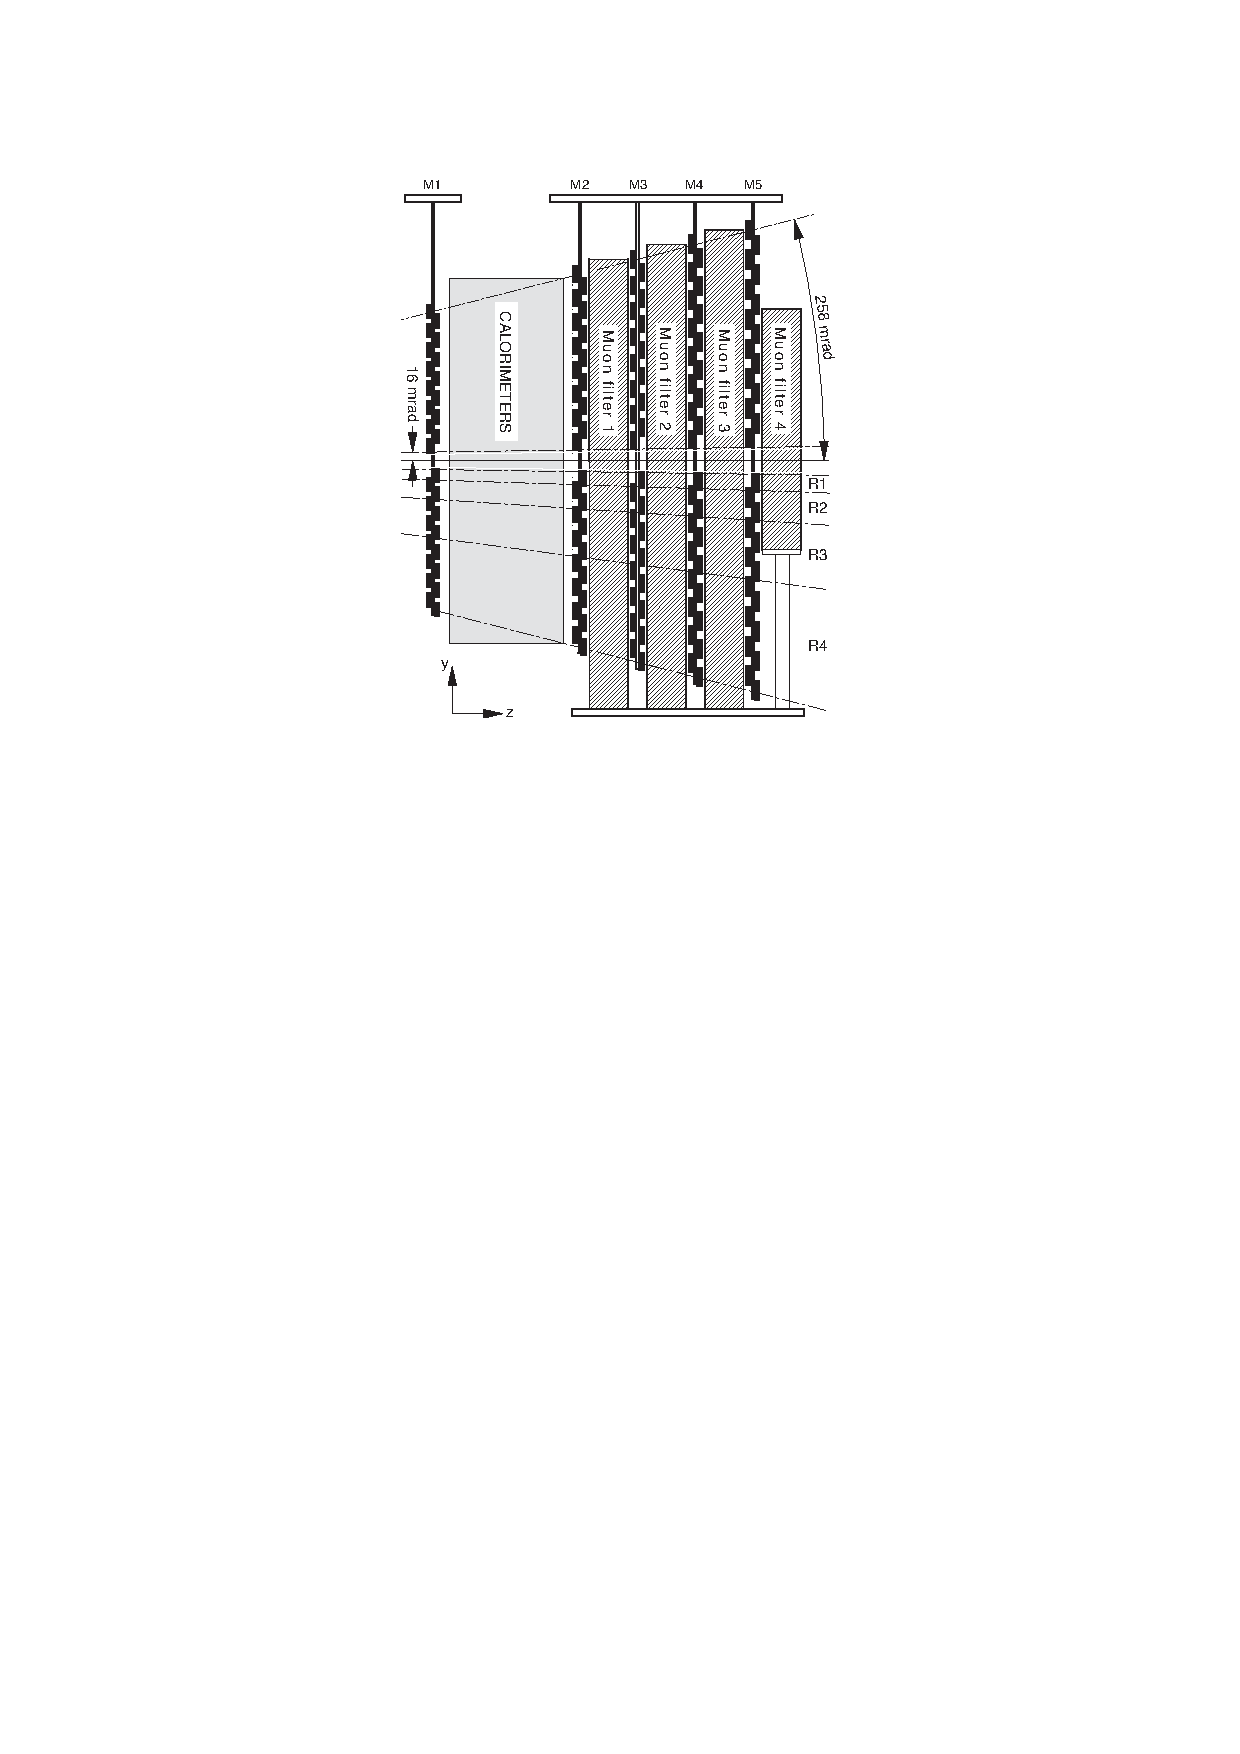
\includegraphics[width=0.4\textwidth]{figs/Detector/muon_layout.pdf}
%     \caption{Schematic of the Muon sub-detector, from Ref.~\cite{Alves:2008zz}.}
%     \label{fig:Dec_muon_schematic}   
% \end{figure}
% %%%%%%%%%%%%%%%%%%%%%%%%%%%%%%%%%%%%%%%%%%%%%%%%%%%%%%%%%%

%%%%%%%%%%%%%%%%%%%%%%%%%%%%%%%%%%%%%%%%%%%%%%%%%%%%%%%%%%
\begin{figure}[!h]
    \centering
    \begin{subfigure}[m]{0.4\textwidth}
        \centering        
        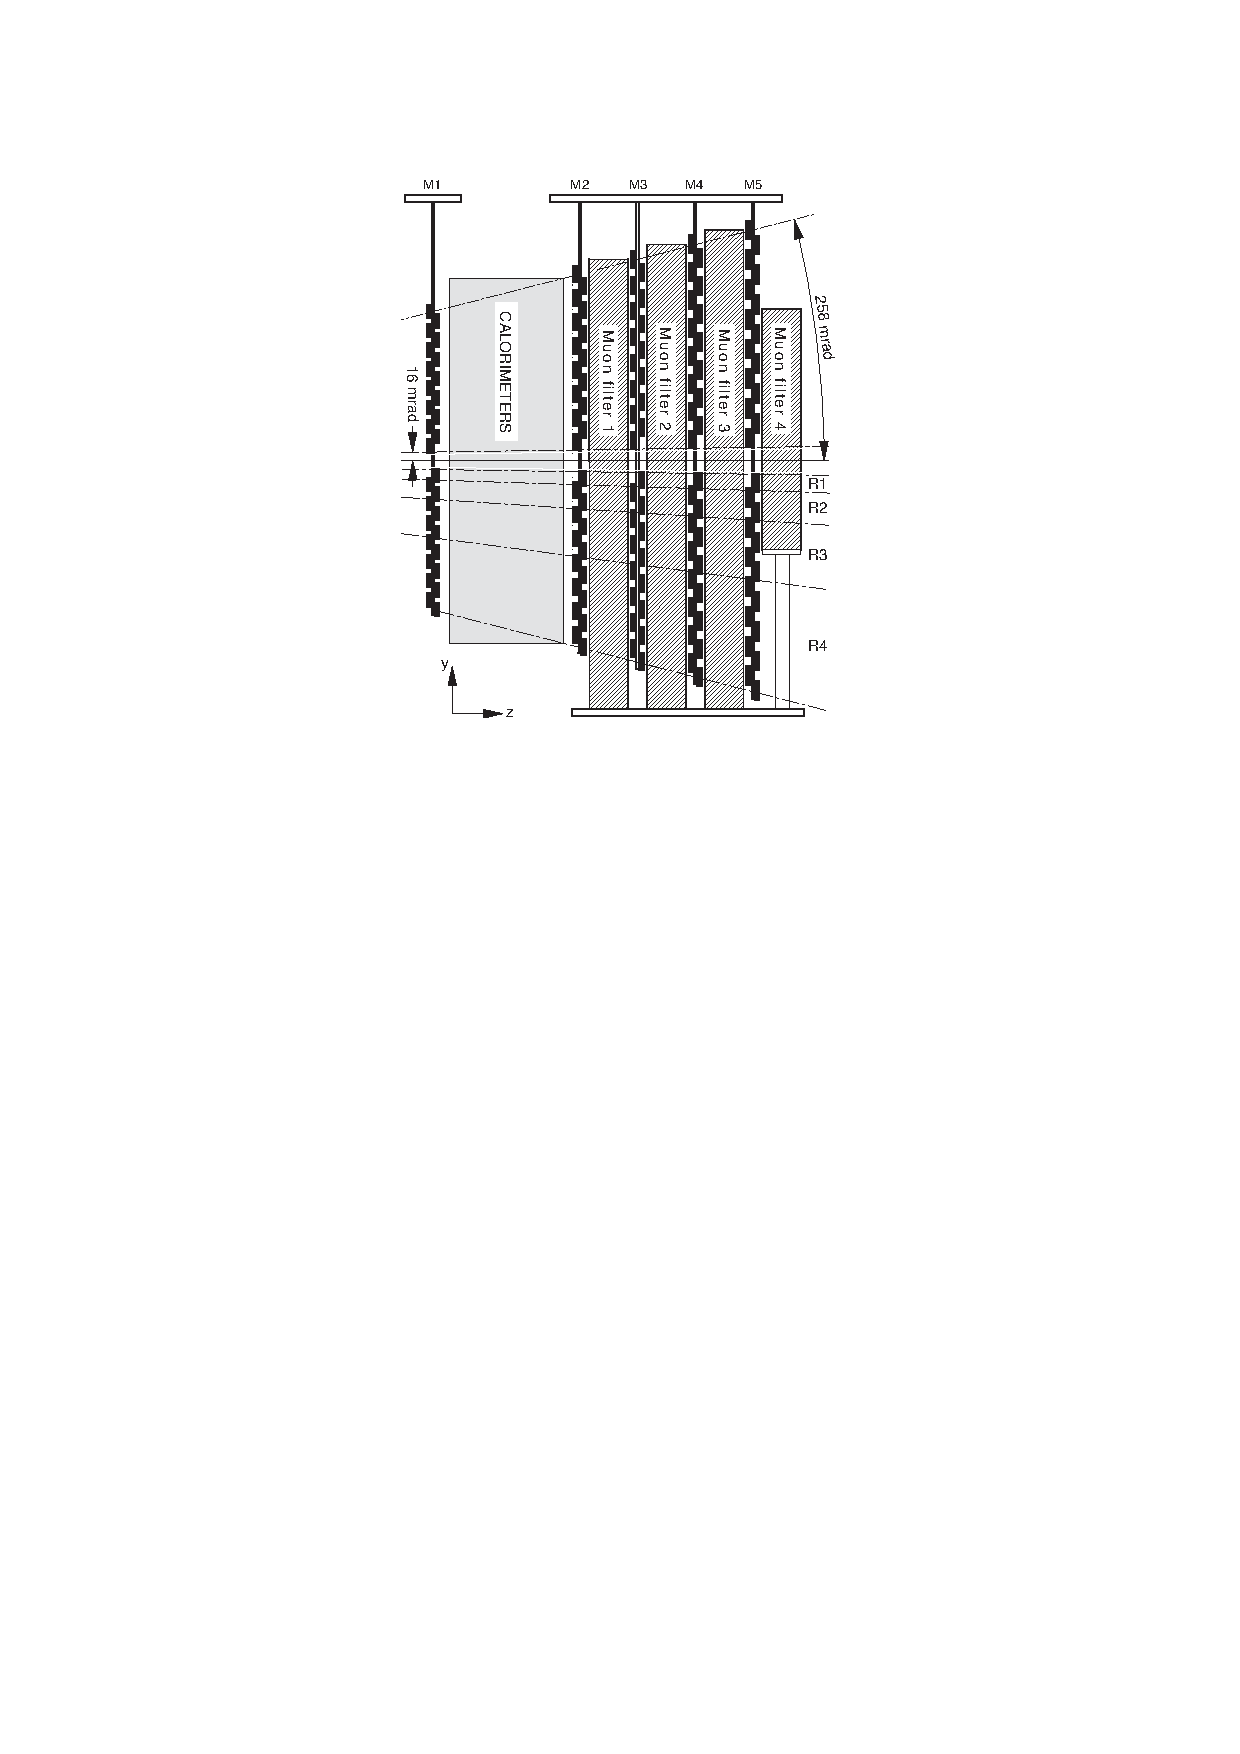
\includegraphics[width=1.0\textwidth]{figs/Detector/muon_layout.pdf}
    \end{subfigure}
    \begin{subfigure}[m]{0.4\textwidth}
        \centering
        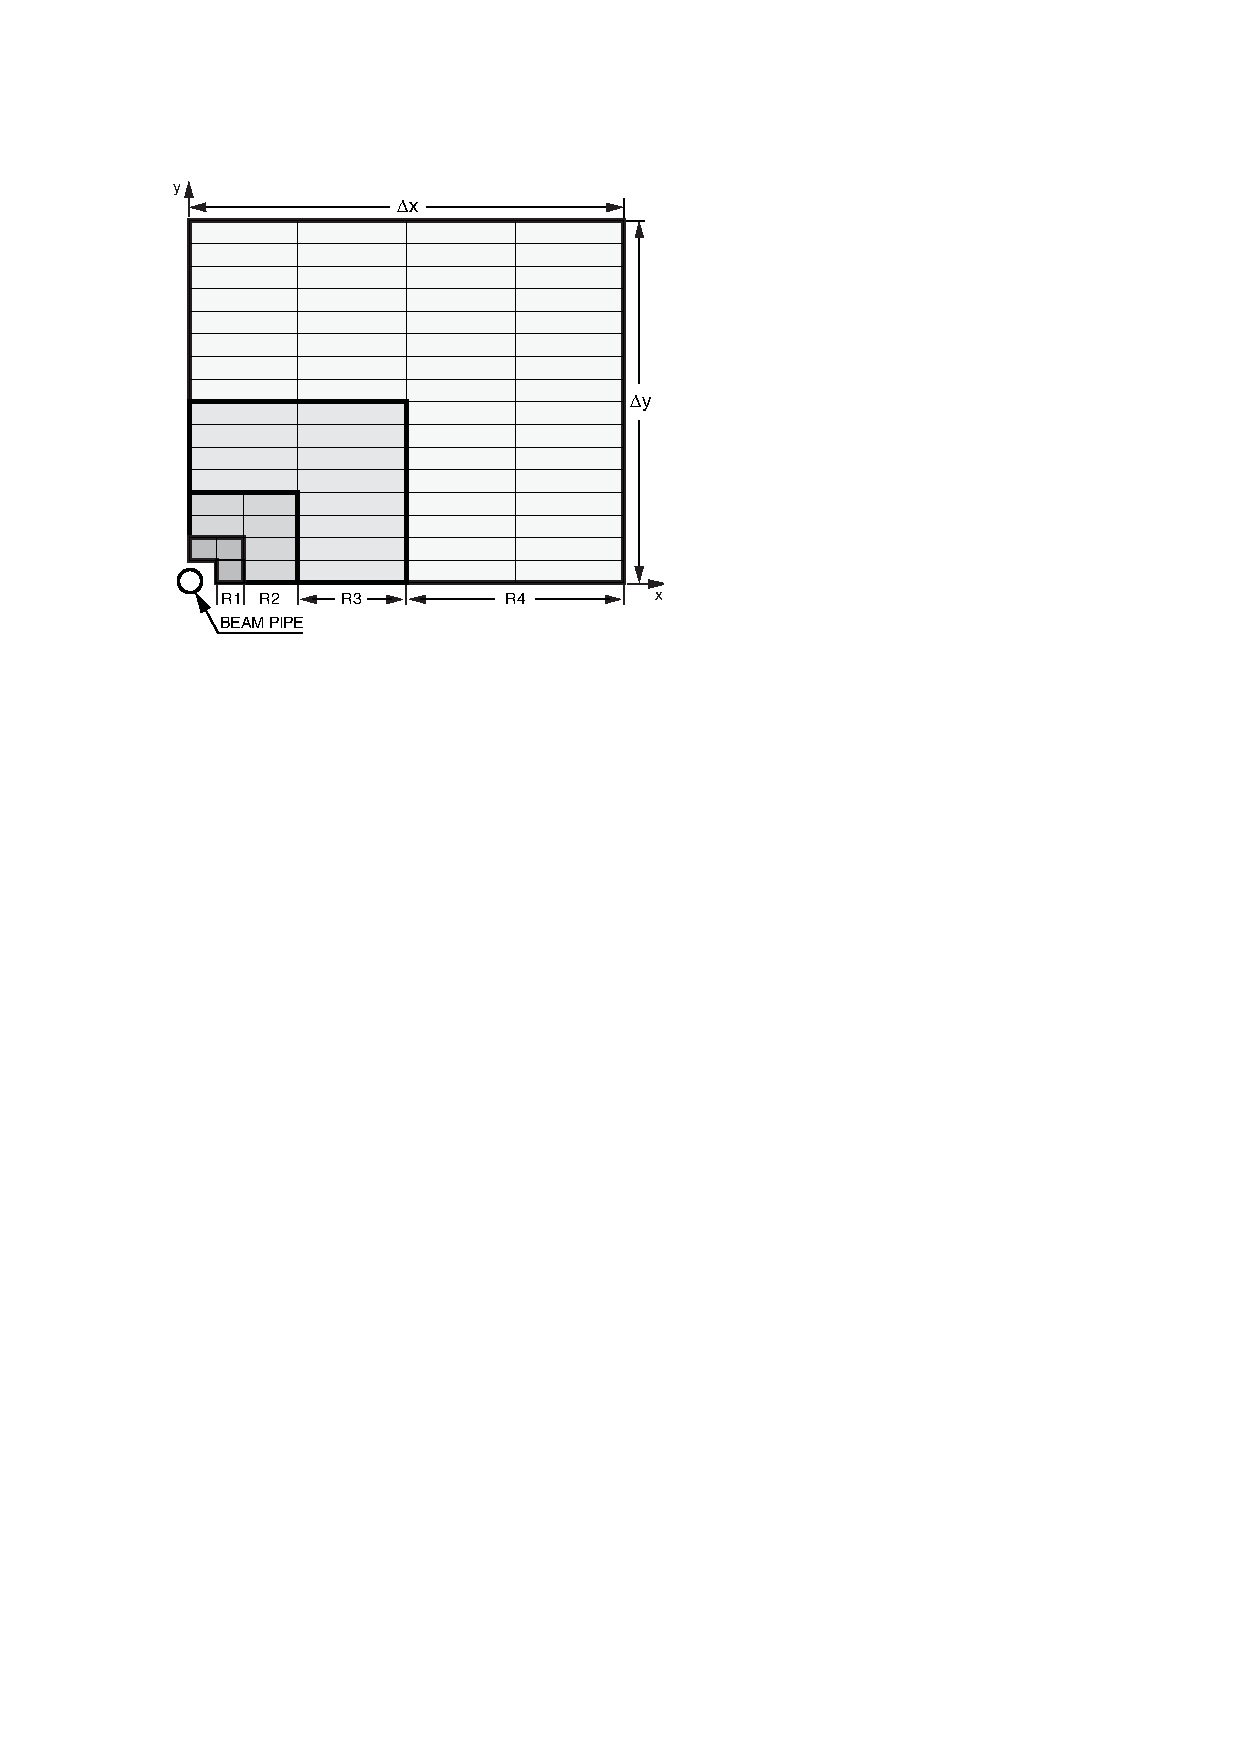
\includegraphics[width=1.0\textwidth]{figs/Detector/muon_cells_layout.pdf}
    \end{subfigure}
    \caption{Side view of the Muon sub-detector (left) and layout of the muon system regions (right), from Ref.~\cite{Alves:2008zz}.}
    \label{fig:Dec_muon_schematic}   
\end{figure}
%%%%%%%%%%%%%%%%%%%%%%%%%%%%%%%%%%%%%%%%%%%%%%%%%%%%%%%%%%

Each of the stations are divided into four regions R1--R4. These are positioned increasingly further from the beam-pipe with increasingly large areas. Each of the regions are segmented into channels; the inner regions have more segmentation than the outer regions such that the particle flux is roughly constant over the four regions.   

The majority of the detector is constructed from Multi Wire Proportional Chambers. These chambers contain a gaseous mixture of carbon dioxide, argon and tetrafluoromethane. When muons pass through this gas they cause ionisation. An array of gold-plated tungsten wires separated by 2\mm are held at a potential difference of around 2.5\,kV with respect to the chamber's conductive walls. The ionised gas and electrons are deflected by the electric field and result in a flow of current. 

Due to the larger flux of particles, the innermost region (R1) of the first station (M1) is instrumented using triple gas electron multiplier detectors. The muons propagating through these detectors ionise a gas mixture made up of argon, carbon dioxide and tetrafluoromethane. The resulting electrons are accelerated toward an anode through three foil layers. The foil layers multiply the number electrons, creating a cascade. 
This type of detector was chosen for the inner region as it is required to be especially radiation hard such that the detector can withstand 10 years of operation.  

\subsection{Trigger}
\label{sec:Dec_trigger}

The primary role of the trigger is to reduce the nominal 40\,MHz beam crossing frequency to a more manageable rate that can realistically be recorded. The trigger is composed to two parts: a custom hardware trigger called Level 1 (\lone) that operates at the nominal 40\, MHz beam crossing rate; and an asynchronous High Level Trigger (\hlt) running software algorithms. These two stages reduce the event rate to around 2\,kHz, exploiting the characteristics of \bquark- and \cquark-hadron decays to preferentially retain signal decays and discard the many uninteresting events.

\subsubsection{Level 1}
The \lone trigger takes input from the muon system, calorimeters and pile-up veto in the \velo. These three systems feed into a single unit to make a global decision about the event. Although the nominal bunch spacing is 25\ns, the \lone decision is made after 4\mus. During this time the detector signals are stored in a \emph{pipeline} buffer. Half of this 4\mus budget is required for the time-of-flight of the particles and delays in the electronics, leaving the \lone trigger 2\mus to reach a decision about each event.  

{\color{Red}
\begin{itemize}
\item talk about derandomizers 
\item thresholds per year
\item where the farm is
\end{itemize}
}

\subsubsection{High Level Trigger}


{\color{Red}
\begin{itemize}
\item Difference between Run 1 and Run 2
\item Mention Turbo in passing
\item farm
\end{itemize}
}


%\subsubsection{High Level Trigger 1}
%\subsubsection{High Level Trigger 2}

\subsection{Reconstruction}
\subsubsection{Charged particle reconstruction}
Charged tracks are reconstructed using the hits in the \velo, \ttracker, \intr and \ot. These are classified into different categories depending on their route taken through the detector as shown in Fig.~\ref{fig:Dec_reco_tracks}. The \intr and \ot are collectively referred to as the T stations. 

\begin{description}
\item \textbf{Long tracks:} these tracks have passed through both \velo and T stations.
\item \textbf{Upstream tracks:} 
\item \textbf{Downstream tracks:} these tracks only contain \ttracker and T station hits. They provide vital information about long-lived particles that decay after they have traversed the \velo. 
\item \textbf{VELO tracks:} these tracks only contain hits in the \velo. They can help improve the primary vertex determination. 
\item \textbf{T tracks:}
\end{description}


%%%%%%%%%%%%%%%%%%%%%%%%%%%%%%%%%%%%%%%%%%%%%%%%%%%%%%%%%%
\begin{figure}[!h]
    \centering
    \begin{subfigure}[m]{0.4\textwidth}
        \centering
        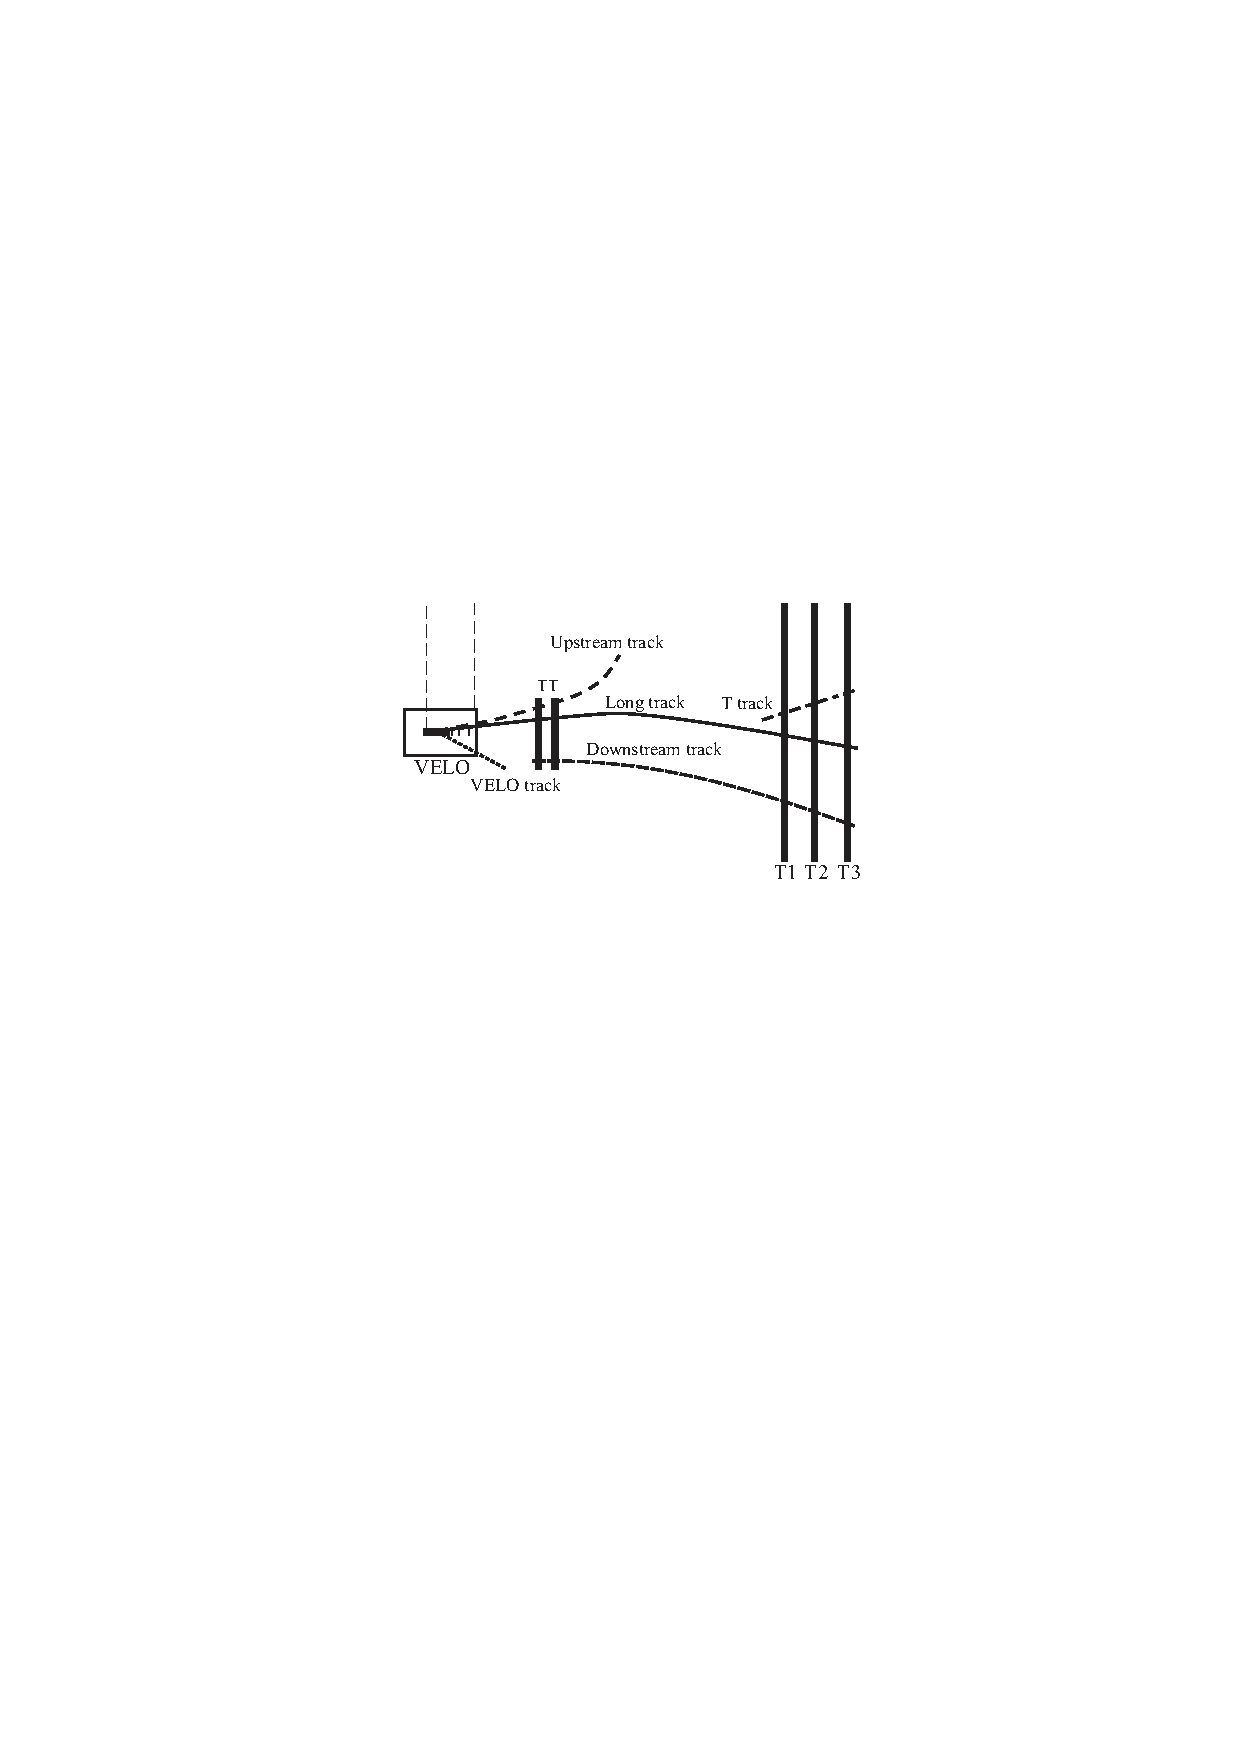
\includegraphics[width=1.0\textwidth]{figs/Detector/reco_track_types.pdf}
    \end{subfigure}
    \begin{subfigure}[m]{0.4\textwidth}
        \centering
        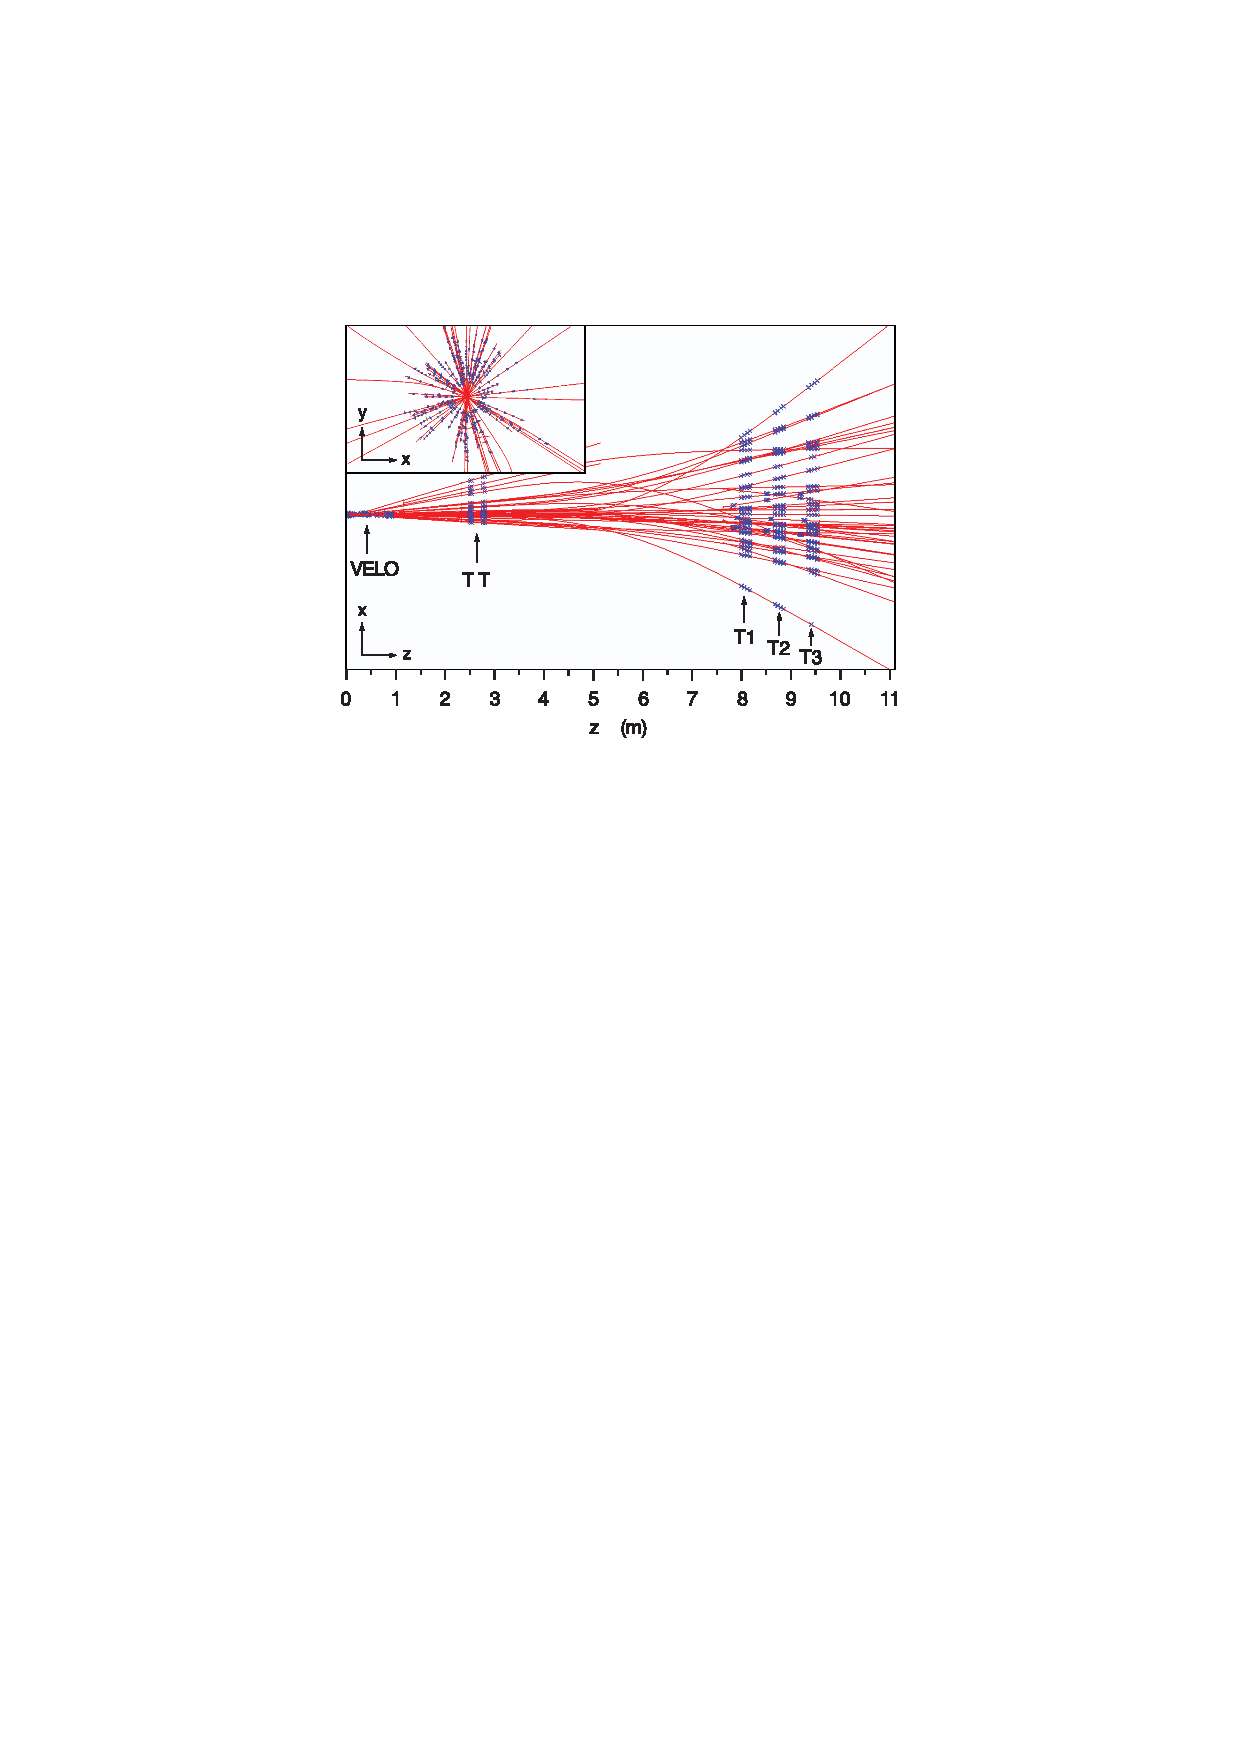
\includegraphics[width=1.0\textwidth]{figs/Detector/reco_track_reco.pdf}
    \end{subfigure}
    \caption{Diagram of the different track reconstruction types (left) and an illustration of the reconstructed tracks in a typical event from Ref.~\cite{LHCb-DP-2014-002}.}
    \label{fig:Dec_reco_tracks}   
\end{figure}
%%%%%%%%%%%%%%%%%%%%%%%%%%%%%%%%%%%%%%%%%%%%%%%%%%%%%%%%%%

\subsubsection{Neutral particle reconstruction}


{\color{Red}
\begin{itemize}
\item photons, \piz, a bit on electrons?
\end{itemize}
}

\section{Luminosity determinations and \velo resolution}
Precise measurements of the recorded luminosity of $pp$ collisions are essential for cross-section measurements. 

\begin{itemize}
\item Van der Meer scans
\item Beam gas imaging
\end{itemize} 

